\PassOptionsToPackage{dvipsnames,svgnames,x11names,table}{xcolor}
\documentclass[a4paper,fleqn]{cas-dc}
\usepackage{tikz}
\usepackage{xcolor}

% ===== REVIEW SWITCH =====================================================
% Text edited in the Nov 2026 revision is wrapped in \edit{...}.
% Review:      \colorlet{editcolor}{edityellow}
% Submission:  \colorlet{editcolor}{black}
\definecolor{edityellow}{HTML}{D4A800}
\colorlet{editcolor}{black}
\newcommand{\edit}[1]{{\color{editcolor}#1}}
% ==========================================================================

% Each upload item starts with \SubmissionPart{name}; its first PDF page is written to
% \jobname.parts, which tools/split_submission.py uses to split the compiled PDF.
\newwrite\partsfile
\immediate\openout\partsfile=\jobname.parts
\newcommand{\SubmissionPart}[1]{\clearpage\thispagestyle{empty}%
  \write\partsfile{#1 \the\ReadonlyShipoutCounter}}
\usepackage{soul}
\soulregister{\hl}{1}
\usetikzlibrary{positioning, calc, backgrounds}
\usepackage{pdflscape}   % for landscape wrapping


% --- Figures & tables ---
\usepackage{graphicx}
\usepackage{booktabs}
\usepackage{multirow}
\usepackage{float}
\usepackage{placeins}
\usepackage{subcaption}
\usepackage{mdframed}
\mdfsetup{nobreak=true} % keep each Finding box in one piece
\usepackage{booktabs}
\usepackage{caption}
\usepackage{listings}
\usepackage{longtable}
\usepackage{array}
\usepackage{pdflscape}
\usepackage{microtype}
% arydshln removed: it breaks tabularx in current TeX Live; tables use \dashedrule.
\usepackage{enumerate}
\usepackage{tabularx}
% --- Lists/columns ---
\usepackage{multicol}
% flushend removed: with current TeX Live it overflowed columns into the footer.
\usepackage{enumitem}
\usepackage{longtable}
% \usepackage{listings}
% --- Colors ---
% \usepackage[dvipsnames,svgnames,x11names]{xcolor}  % merged into line 3 (option clash)

% --- Hyperlinks ---
% \usepackage[colorlinks=true,
%             linkcolor=RoyalBlue,
%             citecolor=ForestGreen,
%             urlcolor=Maroon]{hyperref}


\usepackage{array}
\usepackage{booktabs}
\usepackage{longtable}
\usepackage{xcolor}

\usepackage[most]{tcolorbox}
\usepackage{caption}
\usepackage{xcolor}

\tcbset{
    promptbox/.style={
        enhanced,
        breakable,
        colback=gray!5,
        colframe=black!60,
        boxrule=0.5pt,
        arc=0pt,
        left=6pt,
        right=6pt,
        top=6pt,
        bottom=6pt
    }
}

\newcommand{\dashedrule}{\noalign{\vskip3pt{\color{gray!40}\hrule height 0.4pt}\vskip3pt}}
\newcommand{\tabitem}{\hspace{2pt}\textbullet\hspace{5pt}}


\usepackage{ragged2e}

\newcolumntype{L}[1]{>{\RaggedRight\arraybackslash}p{#1}}

% --- Code listings ---
\usepackage{listings}
\lstset{
  basicstyle=\ttfamily\footnotesize,
  breaklines=true,
  frame=single,
  columns=fullflexible,
  keepspaces=true,
  postbreak=\mbox{\textcolor{gray}{$\hookrightarrow$}\space}
}

% --- REQUIRED for author/affiliation formatting ---
% \usepackage{authblk}

% If the frontmatter runs over more than one page
% use the longmktitle option.

%\documentclass[a4paper,fleqn,longmktitle]{cas-sc}

%\usepackage[numbers]{natbib}
%\usepackage[authoryear]{natbib}
% \usepackage[authoryear,longnamesfirst]{natbib}
\usepackage[numbers]{natbib}
\usepackage{xurl}
% print "Email addresses:" as text instead of the cas icon images, which are not in this repo
\ExplSyntaxOn\bool_gset_true:N \g_stm_nologo_bool\ExplSyntaxOff

%%%Author macros
\def\tsc#1{\csdef{#1}{\textsc{\lowercase{#1}}\xspace}}
\tsc{WGM}
\tsc{QE}
%%%

% Uncomment and use as if needed
%\newtheorem{theorem}{Theorem}
%\newtheorem{lemma}[theorem]{Lemma}
%\newdefinition{rmk}{Remark}
%\newproof{pf}{Proof}
%\newproof{pot}{Proof of Theorem \ref{thm}}

\begin{document}
\let\WriteBookmarks\relax
% Let floats sit with text instead of being deferred to half-empty float pages.
\renewcommand{\topfraction}{0.9}\renewcommand{\dbltopfraction}{0.9}
\renewcommand{\textfraction}{0.07}\renewcommand{\floatpagefraction}{0.7}\renewcommand{\dblfloatpagefraction}{0.7}
\setcounter{topnumber}{3}\setcounter{dbltopnumber}{3}\setcounter{totalnumber}{4}
\renewcommand{\topfraction}{.9}
\renewcommand{\bottomfraction}{.7}
\renewcommand{\textfraction}{.05}
\renewcommand{\floatpagefraction}{.85}
\renewcommand{\dbltopfraction}{.95}
\renewcommand{\dblfloatpagefraction}{.95}
\makeatletter % float pages fill from the top
\setlength{\@fptop}{0pt}\setlength{\@dblfptop}{0pt}
\makeatother
\setcounter{topnumber}{3}
\setcounter{bottomnumber}{2}
\setcounter{totalnumber}{5}
\setcounter{dbltopnumber}{3}
% Short title
\shorttitle{}

% Short author
\shortauthors{N.I. Khan, V. Filkov and R.E. Goldman}

% Suppress the generic CAS preprint footer; retain the page counter.
\ExplSyntaxOn
\cs_set:Npn \__first_footerline: {\mbox{}}
\ExplSyntaxOff

% Main title of the paper
\title[mode = title]{Artificial Intelligence for Angiographic Sequence Analysis: A Systematic Review of Temporal Modeling, Clinical Readiness, and Research Gaps}

\author[1]{Nafiz Imtiaz Khan}[orcid=0000-0003-0149-6012]
\cormark[1]
\ead{nikhan@ucdavis.edu}
\credit{Conceptualization, Methodology, Software, Formal analysis, Investigation, Data curation, Writing -- original draft}


\author[2]{Roger Eric Goldman}[orcid=0000-0003-0394-3744]
\ead{regoldman@health.ucdavis.edu}
\credit{Conceptualization, Methodology, Validation, Supervision, Funding acquisition, Writing -- review \& editing}


\author[1,2]{Vladimir Filkov}[orcid=0000-0003-0492-4393]
\ead{filkov@cs.ucdavis.edu}
\credit{Conceptualization, Supervision, Writing -- review \& editing}


\affiliation[1]{organization={Department of Computer Science, University of California, Davis},
            city={Davis},
            postcode={95616},
            state={CA},
            country={USA}}

\affiliation[2]{organization={Department of Radiology, School of Medicine, University of California, Davis},
            city={Sacramento},
            postcode={95817},
            state={CA},
            country={USA}}

\cortext[1]{Corresponding author}

\begin{abstract}
Digital subtraction angiography (DSA) and fluoroscopy are the reference standard for imaging blood vessels and guiding  endovascular procedures. Angiographic interpretation relies on the temporal pattern of contrast filling and washout. Physicians use the dynamics of the blood flow as an important component of interpretation. How AI methods capture this temporal information has not been systematically examined. We conducted a PRISMA 2020-guided systematic review of AI methods that analyze angiographic image sequences. PubMed/MEDLINE and Semantic Scholar were searched from January 2000 to July 2026, identifying 5,829 records. These records were screened by a large language model (LLM), and two independent human reviewers validated its decisions (inter-rater Cohen's $\kappa=0.98$); after full-text review, 115 studies were included. Another LLM extracted study characteristics and the 44 CLAIM 2024 checklist items, and two human reviewers audited the extraction (97.1\% of audited values correct). Results were synthesized descriptively, without a risk-of-bias tool or meta-analysis. Publications grew sharply after 2020, with 78\% appearing from 2022 to 2026. Cardiac and neurologic applications account for nearly 90\% of studies, and only 4\% combine \edit{DSA} with fluoroscopy. Most studies \edit{(82.6\%)} model temporal information, but half do so with fixed operations rather than learned models. The open question is therefore not whether time is modeled, but how. External validation \edit{(16.5\%),} code release \edit{(21.7\%)} and data release \edit{(2.6\%)} are uncommon, and heterogeneous datasets and metrics prevent comparison of reported performance. We identify twelve research gaps and outline a roadmap toward reproducible, clinically deployable AI for angiography-guided interventions. Funding: RSNA (RSCH2306). Registration: OSF Registries (\url{https://doi.org/10.17605/OSF.IO/6XJK7}).
\end{abstract}


\begin{keywords}
Digital subtraction angiography \sep Fluoroscopy \sep Deep learning \sep Temporal modeling \sep Medical image analysis \sep Interventional radiology \sep Systematic review
\end{keywords}

\maketitle


\section{Introduction}
\label{sec:introduction}

Catheter-based angiography provides real-time visualization of vascular anatomy and pathology and serves as the guidance modality for a wide range of diagnostic and therapeutic procedures spanning vascular disease, trauma, and oncology~\cite{valji2011practice,kaufman2013vascular}. Digital subtraction angiography (DSA) and contrast-enhanced fluoroscopy capture both spatial and temporal information. These sequences show vessel morphology and device position, while contrast arrival and washout provide information about perfusion, collateral circulation, and intervention response that individual frames cannot fully capture~\cite{ACRReporting2024}.

The analysis of such sequences must account for patient motion, differences in acquisition protocols and imaging systems, including variable sequence lengths and contrast administration~\cite{shi2021temporal}. These challenges motivate the design of methods that combine spatial and temporal information to support consistent and appropriate image interpretation and procedural guidance.

\subsection{AI for Angiographic Sequence Analysis}
Artificial Intelligence (AI) methods have been applied to various angiographic tasks, such as image enhancement~\cite{ref152}, vessel segmentation~\cite{ref64}, motion correction~\cite{R2400}, device tracking~\cite{ref99}, lesion assessment~\cite{ref100} and outcome prediction~\cite{ref127}. However, the literature spans clinical and engineering disciplines, with heterogeneous datasets, evaluation protocols, and metrics. This fragmentation makes it difficult to compare approaches or determine how well they generalize across institutions and acquisition settings.

\edit{Studies can capture temporal information in several ways, which raises a central question: how do published studies in this domain use it?} Some may process frames independently, while others combine them through fixed operations such as stacking or registration. Still others may learn dependencies across a sequence. 


\subsection{The Need for a Systematic Review}
Earlier surveys examine deep learning across medical imaging~\cite{Litjens2017,Shen2017} or blood vessel segmentation~\cite{Moccia2018}. Reviews of AI in interventional radiology address planning, guidance, interpretation and clinical workflow~\cite{Iezzi2019,Gurgitano2021,Mukhtar2025}. These perspectives provide clinical and methodological context but do not center on how computational methods analyze angiographic sequences across tasks and applications.

Therefore, a sequence-focused synthesis is needed to connect imaging modalities, anatomical territories, tasks, and architectures with temporal modeling strategies. Evaluation practices, reporting, and reproducibility also require attention because clinical translation depends on transparent methods and evidence of generalization across institutions, vendors and patients~\cite{Tejani2024,collins2024tripod+}.


\edit{To the best of our knowledge, no literature review has yet examined AI methods for angiographic sequences across all of these aspects.}

\subsection{Objectives}
\label{sec:intro-objectives}

This review has four objectives:

\begin{enumerate}[label=\textbf{O\arabic*.}, leftmargin=*, itemsep=4pt]
\item \textbf{Characterize the field:} catalog AI methods, predominantly deep learning, applied to DSA and fluoroscopic sequences across clinical and technical tasks.
\item \textbf{Examine temporal modeling:} identify how temporal information is represented across architectures and applications.
\item \textbf{Assess evidence quality:} review datasets, evaluation practices, reporting, and reproducibility.
\item \textbf{Identify research gaps:} set out directions toward reliable, clinically deployable methods.
\end{enumerate}

This review is intended for clinicians who use angiography, researchers in medical imaging and machine learning, and developers of clinical AI systems.


\section{Methodology}
\subsection{Search Strategy}
\label{sec:search}
This systematic review was conducted in accordance with the Preferred Reporting Items for Systematic Reviews and Meta-Analyses 2020 (PRISMA 2020) guidelines~\cite{Page2021PRISMA}. The review was registered retrospectively on OSF Registries \href{https://doi.org/10.17605/OSF.IO/6XJK7} {https://doi.org/10.17605/OSF.IO/6XJK7}. The completed PRISMA 2020 checklist is provided as Supplementary Table S2. Since the primary objective of this review is to characterize AI methods that operate on angiographic image sequences, the search strategy was designed to jointly capture both the imaging modality and the computational methodology.


Because most clinical articles are indexed by PubMed/\allowbreak MEDLINE \cite{white2020pubmed} and most engineering articles by Semantic Scholar \cite{fricke2018semantic}, we searched these two databases. The search spans publications from \textit{1 January 2000} to the search date, \textit{31 July 2026}. The year 2000 was selected as a practical lower bound because modern digital angiographic workflows and contemporary machine learning approaches largely emerged after this period.

The search query combined two Boolean blocks:

\medskip
\noindent\begin{minipage}{\linewidth}
\noindent\textbf{Block 1: Imaging modality}
\begin{quote}
\small\texttt{(angiograph* OR fluoroscop* OR ``digital subtraction angiography'' OR DSA)}
\end{quote}

\noindent\textbf{AND}

\noindent\textbf{Block 2: Computational methodology}
\begin{quote}
\small\texttt{(``deep learning'' OR ``machine learning'' OR CNN OR transformer OR ``artificial intelligence'' OR AI)}
\end{quote}
\end{minipage}
\medskip


To facilitate reproduction or extension, the database-specific queries, execution dates, filters, and retrieval statistics are given in Appendix~\ref{appendix:search_log}.


\subsection{Eligibility Criteria}
\label{sec:eligibility}
Following PRISMA 2020, we defined explicit inclusion and exclusion criteria, summarized in Table~\ref{tab:criteria}. 

\renewcommand{\arraystretch}{1.25}
\begin{table*}[pos=ht]
\centering
\caption{Eligibility criteria applied at title--abstract screening, with the number of the 5,064 screened records failing each inclusion criterion or excluded on each exclusion criterion in the final screening run. A record can fail several inclusion criteria, so those counts overlap; overall, 4,831 records failed the inclusion gate, 99 were excluded at the exclusion gate and 134 were included.}
\label{tab:criteria}
\begin{tabularx}{\textwidth}{@{}l l X r@{}}
\toprule
\textbf{ID} & \textbf{Type} & \textbf{Criterion} & \textbf{Records} \\
\midrule
I1 & Modality
   & Angiographic imaging: catheter angiography, DSA or contrast fluoroscopy with vessels opacified by an intravascular contrast medium. CT/MR angiography, ultrasound, OCT, retinal imaging and \edit{fluoroscopy outside catheter-based angiographic procedures} do not qualify.
   & 4,154 \\
\dashedrule
I2 & Temporal sequence
   & Temporally ordered multi-frame data (run, series, cine, video or frame sequence) rather than single images only.
   & 4,451 \\
\dashedrule
I3 & Task
   & At least one in-scope computational task (e.g., enhancement, denoising, motion correction, registration, segmentation, detection, classification, tracking, flow or perfusion quantification, outcome prediction), by deep learning, classical machine learning or image processing.
   & 1,098 \\
\dashedrule
I4 & Evaluation
   & The method is evaluated against data (any quantitative result, comparison with a reference, or stated validation procedure).
   & 914 \\
\midrule
E1 & Not full length
   & Conference or meeting abstract, poster or extended abstract without a full methods section.
   & 3 \\
\dashedrule
E2 & Non-research document
   & Editorial, commentary, letter, review, case report, correction, erratum or retraction notice; also set from the PubMed publication type.
   & 95 \\
\dashedrule
E3 & Not in English
   & Full text not available in English.
   & 1 \\
\bottomrule
\end{tabularx}
\end{table*}

We first screened titles and abstracts and retrieved the full text of every record that passed the eligibility criteria. To be included at title--abstract screening, a record had to satisfy four inclusion criteria: (I1) the study uses conventional angiographic imaging, that is, catheter-based angiography (DSA or contrast fluoroscopy in which vessels are opacified by an intravascular contrast medium delivered by the catheter directly into the vessel of interest); (I2) it uses temporally ordered multi-frame data rather than single images; (I3) it addresses at least one in-scope computational task, such as image enhancement, denoising, motion correction, registration, vessel segmentation, lesion detection, classification, tracking, flow or perfusion quantification, or outcome prediction, whether by deep learning, classical machine learning, or traditional image processing; and (I4) it reports an evaluation of the method against data. A record was excluded if (E1) it was an abstract or poster without a full methods section; (E2) it was a non-research document such as an editorial, commentary, letter, review, case report or erratum; or (E3) its full text was not available in English. The inclusion and exclusion criteria judge the content of a record and the form of the publication, respectively.


\subsection{LLM-Assisted Screening Pipeline}
\label{sec:llm-pipeline}

Given the large volume of records available in the searched databases, title--abstract screening was performed by an LLM and the quality of the LLM screening was validated by human reviewers (Section~\ref{sec:validation}). All screening inference was performed locally with the open-weight \texttt{Qwen3.8} model (27B parameters) \footnote{\url{https://ollama.com/library/qwen3.8:27b}} served through the \texttt{Ollama} framework~\cite{marcondes2025using}, which kept the records on local hardware and removed any dependence on external services. We chose a local open-weight model for screening because it is faster and cheaper to run over thousands of records than a large commercial model. Qwen3.8-27B, which is a 27-billion-parameter model released by Alibaba \footnote{https://www.alibabagroup.com/en-US/}, was the strongest and most recent open-weight model that fit on our local server at the time of screening. In prior literature, open-weight models showed high sensitivity in title--abstract screening at no usage cost~\cite{sciurti2025compact}, and models of the Qwen family have previously been used for study selection in systematic reviews~\cite{looareesuwan2026study}.

\subsubsection{Title-Abstract Eligibility Assessment}
\label{sec:title-abstract-sceening}

Screening of database records was performed using two separate LLM calls, one for the inclusion criteria and another for the exclusion criteria. We tailored two prompts for screening against these criteria. In the inclusion criteria prompt, we asked the model to determine which inclusion criteria (I1--I4) were satisfied, while the exclusion criteria prompt asked which exclusion criteria (E1--E3) applied. In both tasks, the model was asked to respond only in yes/no format, with no explanation for its judgment, and responses were obtained in JSON \footnote{https://www.json.org/json-en.html} format. An article was selected for full-text review only if it satisfied all inclusion criteria and met none of the exclusion criteria. Both of the prompts are available in Appendix~\ref{appendix:screening_prompts}.



\subsubsection{Validation of the Screening Pipeline}
\label{sec:validation}

We validated the LLM screening decisions against a human-annotated sample stratified by the pipeline decision. All records \edit{labeled} INCLUDE were reviewed, because each of them changes the review corpus. From the records \edit{labeled} EXCLUDE, we drew a random sample whose size was set by Cochran's formula for a proportion with a finite-population correction~\cite{cochran1977sampling},
\begin{equation}
n_0 = \frac{Z^2\,p(1-p)}{e^2}, \qquad n = \frac{n_0}{1 + \dfrac{n_0-1}{N}},
\end{equation}
where $N$ is the number of excluded records, $Z=1.96$, $p=0.5$ (maximum variance) and $e=0.05$.

Two reviewers, an interventional radiologist and a biomedical AI researcher, \edit{independently screened the title and abstract of every sampled record against the same criteria.} Both of the reviewers had at least 5 years of research experience in their respective fields. If they were unsure about a particular record, the full text of that record was reviewed. We measured the reviewer agreement with Cohen's $\kappa$ \cite{kvaalseth1989note} and resolved disagreements by discussion. The consensus labels formed the gold standard, which served both to evaluate the pipeline and as the final eligibility decision for every sampled record\edit{. Because all LLM-eligible records were sampled, both reviewers checked every record that entered full-text review.}



\subsection{Recurrent Theme Extraction}
We retrieved the full text of all eligible articles and identified research gaps by combining topic modeling with an analysis of each study's stated limitations and future work. We applied Latent Dirichlet Allocation (LDA) \cite{blei2003latent} to the limitations and future work sections of the reviewed studies to identify recurring themes across the included studies. Text preprocessing involved i) lowercasing the text; ii) removing irrelevant content, such as URLs, HTML tags, and reference lists; iii) tokenizing the text into words and removing stop words, such as ``the,'' ``and,'' and ``of''; and iv) lemmatizing words \cite{khyani2021interpretation} to their base \edit{forms, for} example, ``models'' $\rightarrow$ ``model'', ``sequences'' $\rightarrow$ ``sequence.'' Documents were represented using a document--term matrix with bigram features. Next, the number of topics (K) was selected by comparing candidate values from 5 to 20 using the C\_v coherence score~\cite{roder2015exploring}, as in prior topic-model-based systematic reviews~\cite{ogunleye2024systematic}, supplemented by manual assessment of topic interpretability and redundancy. The model used symmetric document--topic and topic--word priors of 1/K each and was trained using Gensim \cite{rehurek2010gensim} with 20 passes, a maximum of 100 iterations per document, and a random seed of 42. \edit{The} \edit{gap framework was built in three steps. First, LDA surfaced recurring topics. Second, one reviewer (a biomedical AI researcher)} interpreted \edit{each} \edit{topic} \edit{from its} 10 highest-weighted terms and representative \edit{studies} and \edit{wrote} the \edit{gap} \edit{definitions, merging topics that described the same problem} and \edit{splitting topics that mixed several;} a \edit{second} \edit{reviewer} \edit{(an} \edit{interventional} \edit{radiologist)} \edit{checked} and \edit{validated} \edit{the} \edit{definitions,} \edit{and} \edit{the} \edit{concerns} raised by the second reviewer were resolved by discussion with the first. Third, the fixed gap definitions (G1--G12) were applied to every included study during data extraction (Section~\ref{sec:full-text-screening}). Supplementary Table~S3 contains the details about the correspondence between topics and gaps. The topics were only a starting point; the gaps themselves result from this careful two-reviewer curation.

\subsection{Data Extraction}
\label{sec:full-text-screening}
We extracted analysis data in a structured format with the help of a reasoning model with high reasoning effort (\texttt{Claude Opus 5.5}). The particular model was selected because it was the most capable model available to us through the institutional Amazon Bedrock platform at the time of extraction. Claude Opus 5.5, released by Anthropic in September 2026, is described by its developer as its strongest Opus model, performing at the level of its frontier model on most work~\cite{anthropic2026opus55}. The use of state-of-the-art (SOTA) commercial models for this purpose has precedent in systematic reviews and meta-analyses \cite{konet2024extraction,khan2025collaborative,reason2024automation}. Each article was processed in a fresh model context holding only the extraction instructions to ensure no information carried over between articles. The extraction schema (provided in Appendix~\ref{appendix:extraction_schema}) covers bibliographic data, imaging modality \& anatomical territory, dataset, tasks, architecture, the temporal-modeling category of the proposed method (Table~\ref{tab:temporal_taxonomy}), validation design, reported metrics, reproducibility, clinical validation, the status of each manually curated research gap, and the 44 items of the CLAIM 2024 checklist~\cite{Tejani2024} \edit{(Table~\ref{tab:claim2024_temporal}). For each gap, the model recorded whether the article documents the gap (states it as a limitation, a motivation or a direction for future work), addresses it with the proposed method, both, or neither, together with a verbatim quote. The evidence count of a gap is the number of studies coded as documenting it; it counts studies that report the problem, not studies that demonstrate it experimentally.}

% Each temporal category and gap assignment had to be backed by a verbatim quote from the article. Every output was validated against the schema, every quote was checked against the article text, and failing outputs were corrected before acceptance. We piloted the protocol on five articles of different types before the full run.

To estimate extraction accuracy, two reviewers independently checked every extracted value of a random sample of studies against the full text and marked each value either correct or incorrect.

\subsection{Statistical Analysis}
\label{sec:stats-methods}
We summarized study characteristics using frequencies and percentages, and reporting completeness against the CLAIM 2024 checklist~\cite{Tejani2024} using proportions with Wilson 95\% confidence intervals~\cite{wilson1927probable}. To assess differences in reporting between publication periods, we compared studies published up to 2024 with those published from 2025 onward. We split at 2025 because the CLAIM 2024 update was published in 2024~\cite{Tejani2024}, so studies from 2025 onward could have followed the updated checklist. We used the comparison as an early check of whether the most recent literature shows any shift toward the updated checklist; a null result indicates that uptake, if any, is not yet visible. We summarized the 44 items within the 14 subsections of the official checklist (e.g., Data, items 7--13); a subsection counts as reported when at least half of its applicable items are reported. The comparison used a two-sided Fisher's exact test for each subsection~\cite{fisher1922interpretation}, with Holm correction for multiple comparisons across subsections~\cite{holm1979simple}.

To characterize overlap between task categories, we computed the Tanimoto distance between the sets of studies assigned to each pair of categories, considering both primary and secondary tasks~\cite{rogers1960tanimoto}. We then performed hierarchical clustering using average linkage, also known as the unweighted pair-group method with arithmetic mean (UPGMA)~\cite{sokal1958statistical}. This analysis summarizes relationships based on shared study membership, conceptually related to co-occurrence-based bibliometric mapping~\cite{vaneck2010software}.

Reported performance metrics were summarized using histograms. Because datasets, validation protocols, and evaluation metrics differed substantially across studies, we did not perform a meta-analysis. 

\section{Results}
\label{sec:analysis}
\label{sec:results}
This section contains the methodological results and the analyses of the selected articles. We first report study selection and the validation of screening and extraction, then the characteristics of the \edit{115} included studies: publication trends, modalities and territories, tasks and architectures, temporal modeling, venues, reported performance and reporting quality.

\subsection{Study Selection and Review Corpus}
The screening search identified 5,829 records (PubMed/\allowbreak MEDLINE 4,071; Semantic Scholar 1,758). After removing 765 duplicates, 5,064 records remained. The LLM \edit{labeled} 134 as eligible and excluded 4,930. 4,831 failed at least one inclusion criterion and 99 met an exclusion criterion (E1: 3, E2: 95, E3: 1). The PRISMA diagram of this eligibility analysis is shown in Figure~\ref{fig:prisma}.

Applying Cochran's \cite{cochran1977sampling} formula, we set the validation sample at 357 of the 4,930 exclusions; we also included all the LLM-eligible articles, which resulted in 491 records for manual review.

The two reviewers agreed on 487 of the 491 records (99.2\%; Cohen's $\kappa=0.978$, 95\% CI 0.957--0.999). The four cases with disagreements were resolved through discussion by the annotators. The resultant data, after resolution of the disagreements, served as the manually validated dataset.

The manually validated dataset contained 122 eligible reports (14 LLM-eligible records were excluded, while 2 LLM-non-eligible records were added) for review. Full text could not be retrieved for 2 of \edit{these, so 120 reports were assessed at full text. During full text analysis, we found that two of them were published meeting abstracts without a full methods section, so they were excluded under E1. Of} the \edit{remaining} \edit{118 reports, three were earlier versions (two preprints and one conference paper) of an included journal article; we counted each study once, using} the \edit{journal version. The} final review corpus \edit{therefore} comprises \edit{115} studies. 

% All 491 screening decisions are listed in Supplementary Table~S1.


The full-text LLM extraction audit covered 6 of the \edit{115} studies (5\%) and 444 values. Each study contained 74 fields: 18 study-level fields, the status of the 12 research gaps, and 44 CLAIM-informed reporting criteria. Disagreements were resolved through discussion to obtain the final validated set. Inter-annotator agreement was \(\kappa = 0.967\). Compared with the validated set, 431 of 444 extracted values were correct (97.1\%).




\begin{figure*}[pos=htbp]
  \centering
  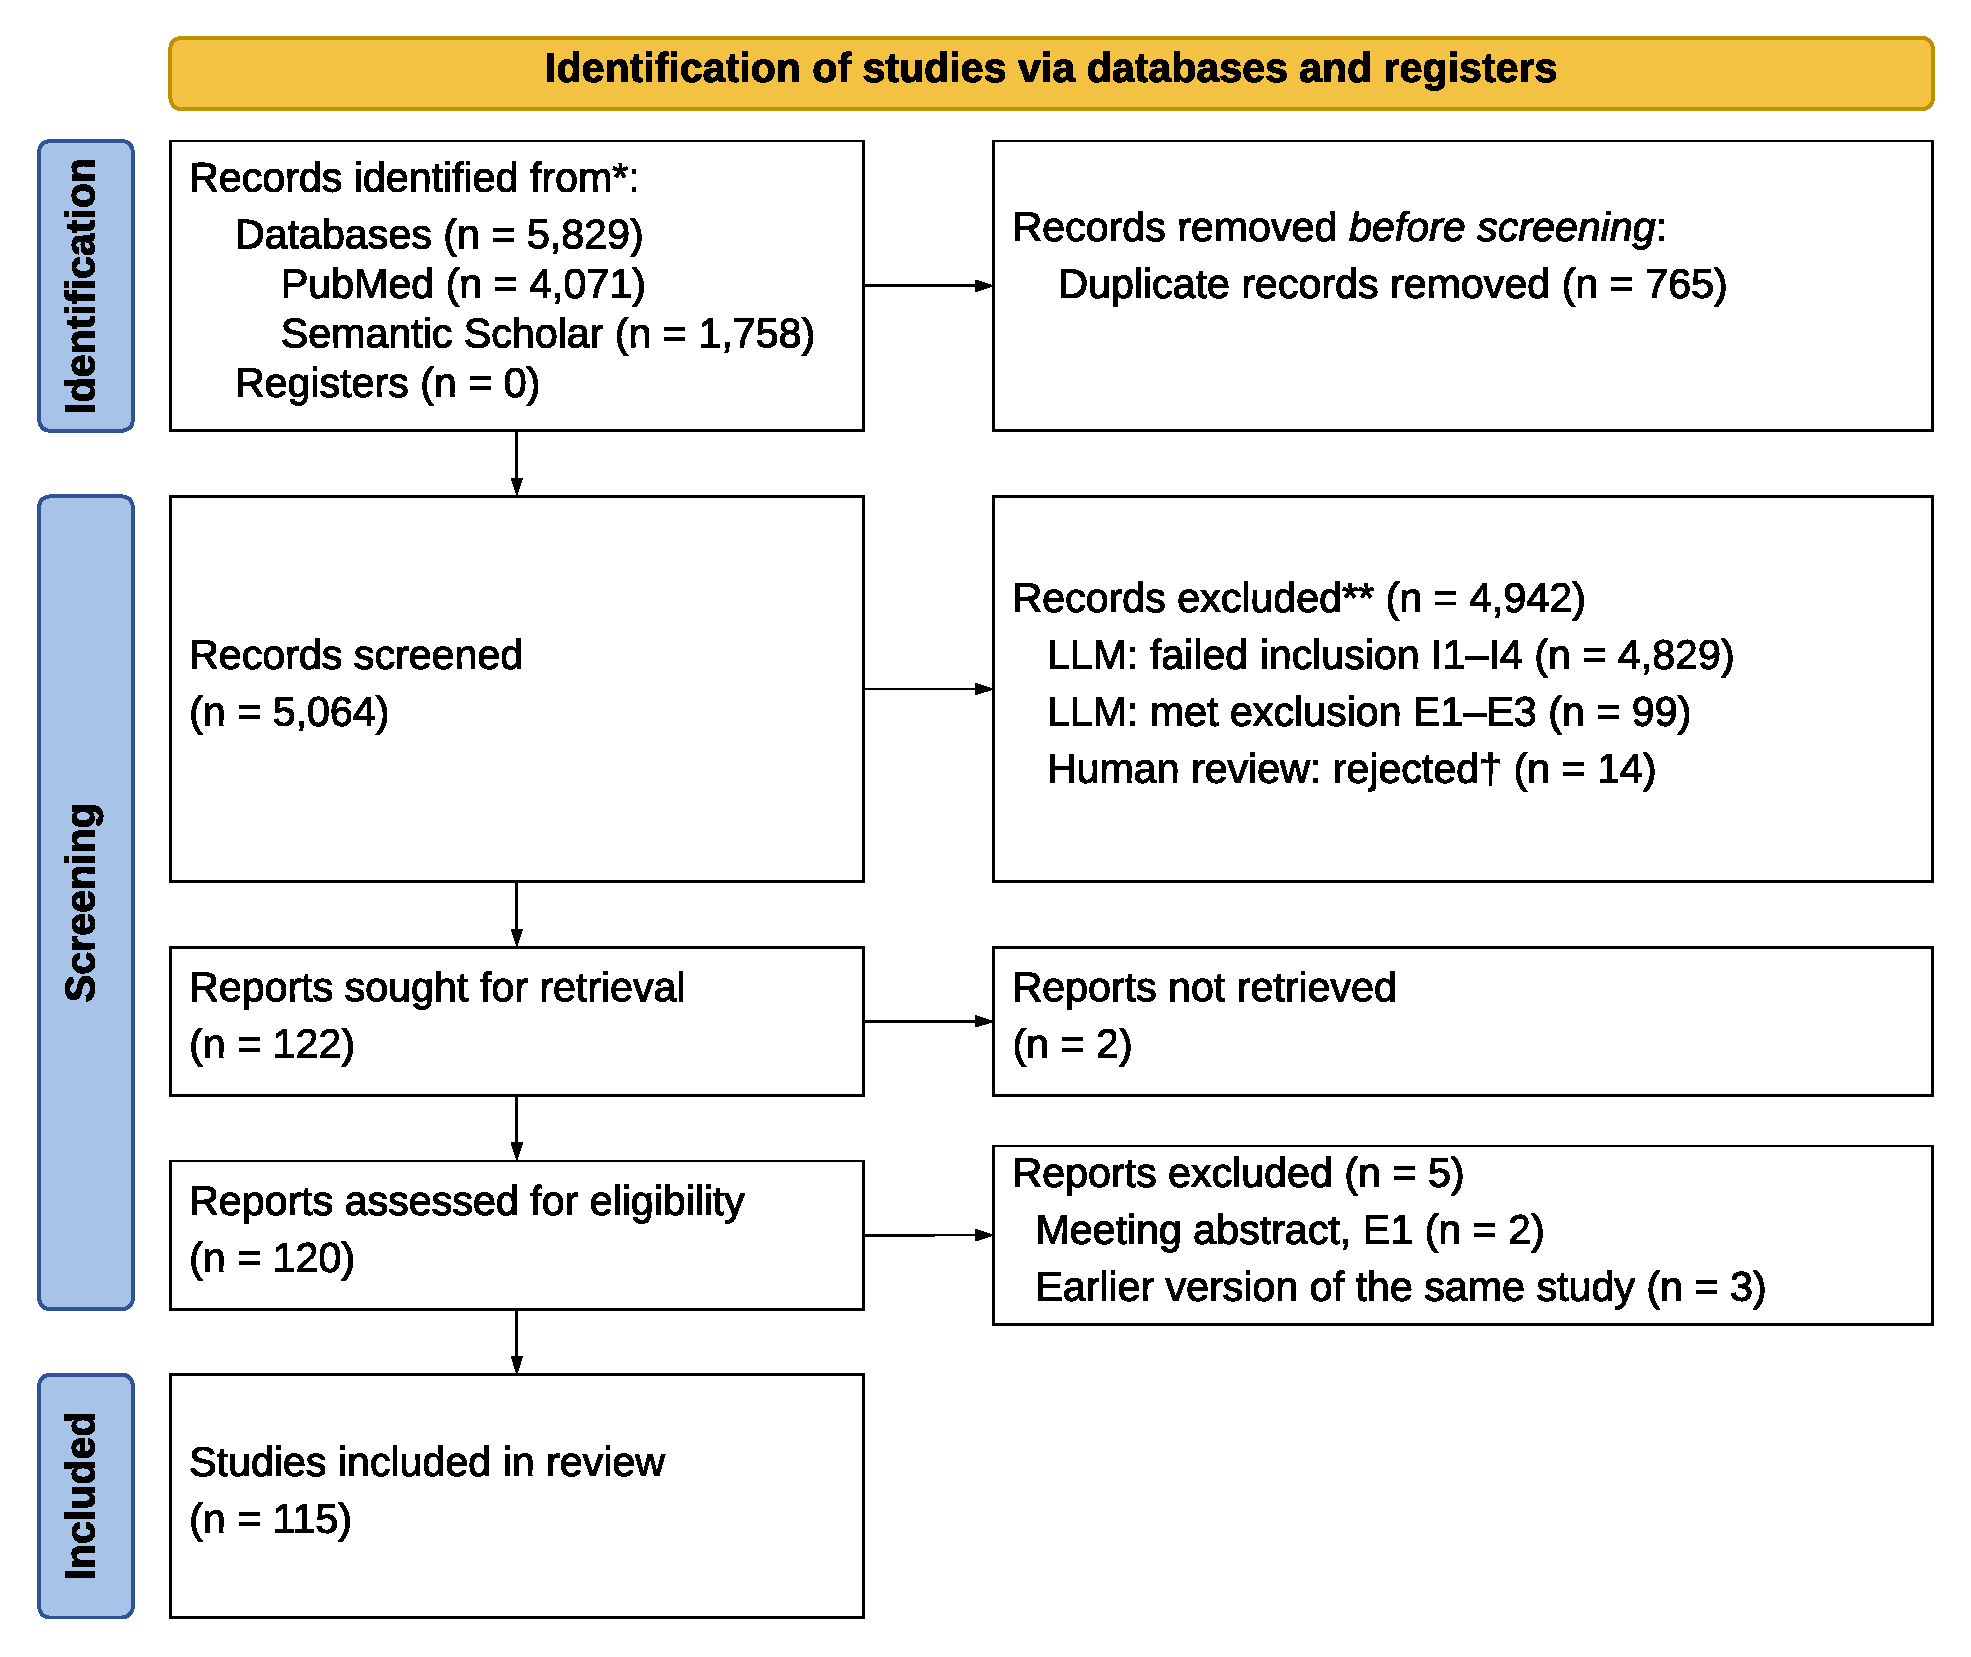
\includegraphics[width=\textwidth, height=13.6cm]{figs/prisma.pdf}
  \caption{PRISMA 2020 flow diagram of study identification, screening, eligibility assessment and inclusion. *PubMed/MEDLINE and Semantic Scholar. **Title/abstract screening by the LLM pipeline (Section~\ref{sec:llm-pipeline}), followed by independent dual human review of all 134 LLM-eligible records and a random sample of 357 LLM-excluded records (Cohen's $\kappa=0.978$; disagreements resolved by discussion, Section~\ref{sec:validation}). $^{\dagger}$LLM-eligible records judged ineligible by the reviewers. Two records excluded by the LLM (both on criterion I2) were judged eligible by the reviewers and are counted among the 122 reports sought for retrieval. Full text could not be retrieved for 2 of the \edit{122. Of the 120 reports assessed, 5 were excluded: 2 meeting abstracts (E1) and 3 earlier versions (preprint or conference paper) of studies already included through their journal article,} so \edit{115} studies were included.}
  \label{fig:prisma}
\end{figure*}



\subsection{Publication Trends}
\label{subsec:trends}
\begin{figure}[pos=!htbp]
\centering
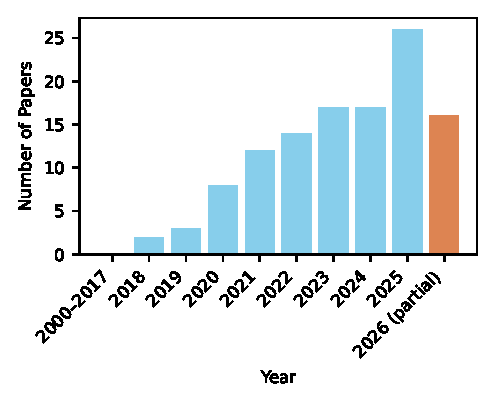
\includegraphics[width=1\linewidth]{figs/temporal_trends.pdf}
\caption{Included studies by publication year. The 2026 bar covers a partial year.}
\label{fig:temporal_trends}
\end{figure}

The trend of the selected articles,  Figure~\ref{fig:temporal_trends}, shows that no included study predates 2018, and only five appeared in 2018--2019. Output rose sharply after 2020 and stayed high through the study inclusion end date. The partial year 2026 already exceeds several earlier full years. 


% Transformer-based temporal models appeared later; all ten such studies were published from 2023 onward.

\vspace{0.25cm}
\begin{mdframed}[linewidth=0.5pt, linecolor=black, backgroundcolor=blue!10]
\textbf{Finding 1.} The field is still growing: 78\% of studies \edit{(90/115)} were published from 2022 to 2026.
\end{mdframed}
\vspace{0.25cm}

\subsection{Imaging Modalities and Anatomical Coverage}
This subsection summarizes the imaging modalities used by the included studies and the anatomical territories they address. The anatomical distribution is shown in Figure~\ref{fig:anatomy_distribution}.


X-ray/fluoroscopy \edit{(55} studies, 48\%) and DSA \edit{(54,} 47\%) are almost equally common, but they are rarely studied jointly: only 5 studies (4\%) use both. Cardiac \edit{(46\%)} and neurologic (41\%) applications, which include cerebral and spinal vascular territories, make up nearly 90\% of the corpus, while abdominopelvic, peripheral, and other thoracic territories are rare (Figure~\ref{fig:anatomy_distribution}). \edit{Most studies develop and test their models within a single territory, so whether} models trained on coronary or cerebral angiography transfer to other vascular regions \edit{remains} \edit{largely} \edit{untested.}

\vspace{0.25cm}
\begin{mdframed}[linewidth=0.5pt, linecolor=black, backgroundcolor=blue!10]
\textbf{Finding 2.} Studies use DSA or X-ray/\allowbreak fluoroscopy in nearly equal numbers but almost never both, and nearly 90\% address cardiac or neurologic territories.
\end{mdframed}
\vspace{0.25cm}






\label{subsec:modality_anatomy}
\begin{figure}[pos=!htbp]
\centering
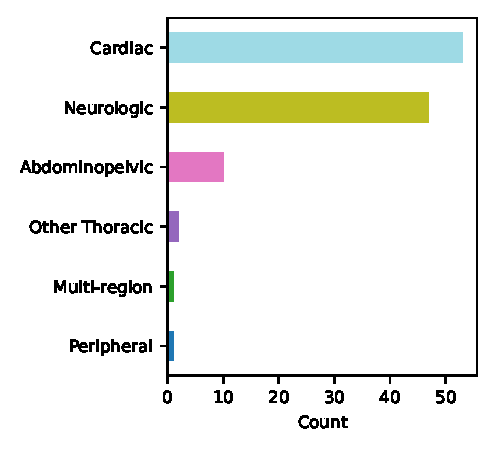
\includegraphics[width=1\linewidth]{figs/anatomy_distribution.pdf}
\caption{Anatomical distribution across included studies. The Neurologic category includes cerebral and spinal vascular territories.}
\label{fig:anatomy_distribution}
\end{figure}


% -----------------

\subsection{Computational Tasks and Model Architectures}
Here, we examined the computational tasks addressed by the included studies and the model architectures used to perform them. We categorized studies by their primary task and summarized the architectures used within each category to characterize the methodological focus of the literature. Figure~\ref{fig:task_distribution} presents the distribution of primary tasks across the \edit{115} studies, while Table~\ref{tab:task_architecture_clean} summarizes the corresponding architectures.
\renewcommand{\arraystretch}{1.25}
\begin{table*}[pos=ht]
\centering
\caption{Temporal-modeling categories of the proposed method in each of the \edit{115} included studies, each assignment backed by a verbatim quote from the article.}
\label{tab:temporal_taxonomy}
\begin{tabularx}{\textwidth}{@{}l X r r@{}}
\toprule
\textbf{Category} & \textbf{Operational Definition} & \textbf{N} & \textbf{\%} \\
\midrule
No Temporal Use
  & Each frame is processed \edit{independently;} no \edit{information} \edit{is} \edit{combined} across frames.
  & \edit{20} & \edit{17.4\%} \\
\dashedrule
Frame Aggregation
  & \edit{Frames} are combined \edit{by} \edit{a} \edit{fixed} \edit{operation} (channel stacking, concatenation, \edit{differencing,} \edit{averaging or temporal pooling)} before a 2D model. \edit{A model trained on stacked frames can learn short-range cross-frame relations, but the sequence has no dedicated temporal mechanism.}
  & \edit{16} & \edit{13.9\%} \\
\dashedrule
Optical Flow / Registration
  & Explicit frame-to-frame motion estimation, registration, or classical tracking/association (e.g., optical flow, particle filters, cross-correlation).
  & 19 & \edit{16.5\%} \\
\dashedrule
RNN / LSTM / GRU
  & Recurrent architectures (LSTM, GRU, ConvLSTM, recurrent residual modules) propagate a hidden state across the sequence.
  & \edit{16} & \edit{13.9\%} \\
\dashedrule
3D CNN / Video Model
  & 3D or spatiotemporal convolutions, or video-/sequence-level representation learning, treating the sequence as a joint spatiotemporal volume.
  & \edit{19} & \edit{16.5\%} \\
\dashedrule
Transformer / State-Space
  & Self-attention or state-space mechanisms modeling long-range dependencies across frames.
  & 10 & \edit{8.7\%} \\
\dashedrule
Hemodynamic / Physics-Informed
  & Explicit physiological or physics-based temporal modeling (reduced-order flow models, hemodynamic priors, time-density curve modeling).
  & 15 & \edit{13.0\%} \\
\midrule
\edit{\textbf{Total}} & & \edit{\textbf{115}} & \edit{\textbf{100.0\%}} \\
\bottomrule
\end{tabularx}
\end{table*}

\renewcommand{\arraystretch}{1.2}
\begin{table}[pos=!htbp]
\centering
\small
\caption{Share of studies using explicit temporal modeling (any category in Table~\ref{tab:temporal_taxonomy} except ``No Temporal \edit{Use'')} by primary task, modality and territory. Rows with fewer than 5 studies are omitted: Background Subtraction (4); Other task (1); Other modality (1); Peripheral (1); Other Thoracic (incl. aortic) (2); Multi-region (1); Not reported (1).}
\label{tab:temporal_crosstab}
\begin{tabularx}{\columnwidth}{@{}X r r@{}}
\toprule
\textbf{Dimension} & \textbf{N} &
\shortstack[r]{\textbf{Temporal-Use}\\\textbf{Rate}} \\
\midrule
\multicolumn{3}{@{}l}{\textit{By Primary Task}} \\
\dashedrule
Temporal Sequence \edit{Modeling} & 6 & 100\% \\
Contrast Flow Analysis & \edit{8} & \edit{100\%} \\
Outcome Prediction & 9 & 89\% \\
Image Enhancement \& Denoising & 9 & 89\% \\
\edit{Vessel} \edit{Segmentation} & \edit{15} & \edit{87\%} \\
\edit{Disease} \edit{Classification} \& \edit{Grading} & \edit{29} & \edit{83\%} \\
Motion Correction \& Registration & 9 & 78\% \\
Object Detection \& \edit{Localization} & \edit{16} & \edit{69\%} \\
Catheter \& Device Tracking & 9 & 67\% \\
\midrule
\multicolumn{3}{@{}l}{\textit{By Imaging Modality}} \\
\dashedrule
DSA & \edit{54} & \edit{87\%} \\
X-ray / Fluoroscopy & \edit{55} & \edit{80\%} \\
DSA + Fluoroscopy (both) & 5 & 60\% \\
\midrule
\multicolumn{3}{@{}l}{\textit{By Anatomical Territory}} \\
\dashedrule
Neurologic & \edit{47} & \edit{91\%} \\
Cardiac & \edit{53} & \edit{79\%} \\
Abdominopelvic & 10 & 60\% \\
\bottomrule
\end{tabularx}
\end{table}
\begin{table*}[pos=t]
\centering
\small
\begin{tabularx}{\textwidth}
{>{\raggedright\arraybackslash}p{4.4cm}
 >{\raggedright\arraybackslash}X}
\toprule
\textbf{Task} & \textbf{Representative Architectures} \\
\midrule

Disease Classification \& Grading (\edit{$n=29$})\newline{\footnotesize\itshape disease label or severity grade} &
CNN classifiers \edit{(16),} recurrent (LSTM/GRU) (5), hybrid CNN--Transformer (3). Examples: DeepRV~\cite{ref198}, ResNet101~\cite{R0099}, X3D~\cite{ref102}, SeqCon~\cite{ref91}, YOLOv8~\cite{R0521}, ResNet-50~\cite{ref161} \\[6pt]

Object Detection \& Localization (\edit{$n=16$})\newline{\footnotesize\itshape locating lesions, stenoses or landmarks} &
object detectors \edit{(9),} hybrid CNN--Transformer \edit{(3), U-Net/encoder--decoder (2).} Examples: YOLOv10x~\cite{R0058}, YOLO Attention~\cite{R0570}, UOA Detector~\cite{ref190}, 2D ResUNet++~\cite{ref20}, 2D convolutional neural network~\cite{R1213}, LT-YOLO~\cite{R1222} \\[6pt]

Vessel Segmentation ($n=15$)\newline{\footnotesize\itshape pixel-wise delineation of vessels} &
U-Net/encoder--decoder (14), hybrid CNN--Transformer (1). Examples: DOSTA-Net~\cite{ref64}, TCA-Net~\cite{ref2}, nnU-Net~\cite{ref15}, TVS-Net~\cite{ref34}, U-Net++~\cite{ref211}, ATFNet~\cite{R1674} \\[6pt]

Catheter \& Device Tracking ($n=9$)\newline{\footnotesize\itshape following devices across frames} &
U-Net/encoder--decoder (5), other learned models (2), hybrid CNN--Transformer (2). Examples: Stent-RD-UNet~\cite{ref178}, Neuro-Vascular Assist~\cite{R1362}, TAG-DL~\cite{ref56}, ConTrack~\cite{R3149}, U-Net~\cite{ref79}, Improved U-Net~\cite{ref162} \\[6pt]

Contrast Flow Analysis (\edit{$n=8$})\newline{\footnotesize\itshape perfusion or flow from contrast} &
CNN classifiers \edit{(3), U-Net/encoder--decoder} (3), other learned models (2). Examples: custom convolutional neural network~\cite{R0100}, perfDSA~\cite{ref28}, YOLOv8m~\cite{R1680}, ResNet~\cite{ref43}, Physics-informed neural network~\cite{R2786} \\[6pt]

Image Enhancement \& Denoising ($n=9$)\newline{\footnotesize\itshape improving image quality or reducing dose} &
other learned models (4), U-Net/encoder--decoder (3), hybrid CNN--Transformer (2). Examples: SAVE-Net~\cite{ref152}, GenDSA~\cite{ref39}, SepConv++~\cite{ref51}, GaraMoSt~\cite{R2490}, MoSt-DSA~\cite{ref104}, ASRNet~\cite{R3126} \\[6pt]

Motion Correction \& Registration ($n=9$)\newline{\footnotesize\itshape aligning frames, views or modalities} &
U-Net/encoder--decoder (4), other learned models (4), non-learning (1). Examples: VGG encoders~\cite{R2400}, Residual U-Net~\cite{ref227}, 4DRGS~\cite{R2466}, TiAVox~\cite{R3164}, SSDR network~\cite{R3338}, RAFT~\cite{ref74} \\[6pt]

Outcome Prediction ($n=9$)\newline{\footnotesize\itshape predicting a clinical outcome or event} &
classical ML (5), other learned models (2), hybrid CNN--Transformer (1). Examples: hybrid transformer-UNet~\cite{ref42}, XGBoost~\cite{ref127}, CLIP ViT-B/32~\cite{R0643}, Deep neural network~\cite{R1263}, logistic regression~\cite{R1503}, gradient boosting classifier~\cite{R1609} \\[6pt]

Temporal Sequence Modeling ($n=6$)\newline{\footnotesize\itshape sequence itself is the output, e.g., phase detection} &
recurrent (LSTM/GRU) (2), CNN classifiers (2), generative (GAN/diffusion) (1). Examples: CDKD-w+~\cite{ref36}, STA-IPCon~\cite{ref57}, Auxiliary Input in Training~\cite{R2411}, ResNet-50~\cite{ref148}, U-Net-like vesselness network~\cite{ref95}, MGR-Net~\cite{ref96} \\[6pt]

Background Subtraction ($n=4$)\newline{\footnotesize\itshape producing DSA-like subtracted images} &
other learned models (1), U-Net/encoder--decoder (1), generative (GAN/diffusion) (1). Examples: HyperMorph~\cite{ref40}, 3D U-Net~\cite{ref52}, pix2pix~\cite{ref93}, rigid registration with mutual information~\cite{R4804} \\[6pt]

Other ($n=1$)\newline{\footnotesize\itshape none of the above} &
other learned models (1). Examples: AngioPlus Core~\cite{R3052} \\[6pt]

\bottomrule
\end{tabularx}
\caption{Architecture families by primary task. Each task is shown with a short definition and $n$, the number of studies; the three most frequent families are listed with study counts, followed by up to six named architectures with the studies that use them.}
\label{tab:task_architecture_clean}
\end{table*}



Figure~\ref{fig:task_distribution} shows that disease classification and grading is the most common primary task \edit{(29} of \edit{115} studies), followed by object detection \& localization \edit{(16)} and vessel segmentation (15). Regarding the model architectures (Table~\ref{tab:task_architecture_clean}) involved in those tasks, 14 of the 15 segmentation studies use encoder--decoder models, mostly U-Net variants; detection studies use YOLO, DETR and R-CNN detectors on ResNet backbones; classification relies on ResNet-style CNNs, with Transformers increasingly added. The majority of architectures are adapted from natural-image computer vision rather than designed specifically for angiography.

Tasks that produce a temporal output remain uncommon. These included temporal sequence modeling, such as cardiac cycle detection and key-frame identification (6 studies), and contrast flow analysis \edit{(8} studies). Many spatial tasks, such as segmentation, detection, and classification, use several frames only to stabilize a per-frame prediction (discussed in detail in Section~\ref{subsec:temporal_taxonomy}).


\label{subsec:tasks_architectures}
\begin{figure*}[pos=!tp]
\centering
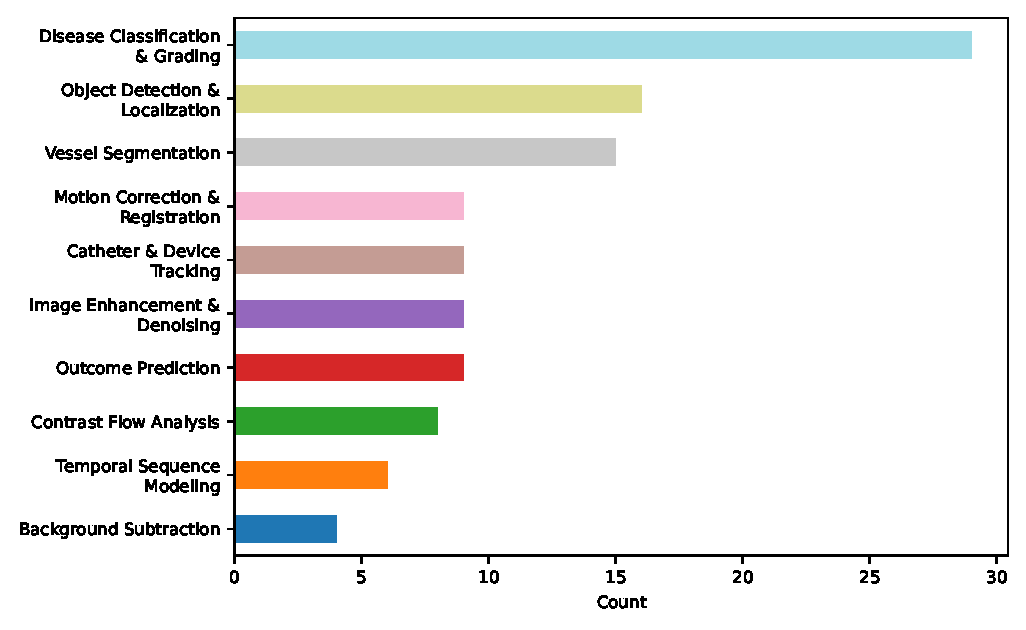
\includegraphics[width=1\linewidth]{figs/task_distribution.pdf}
\caption{Distribution of primary computational tasks across included studies. Task definitions are given in Table~\ref{tab:task_architecture_clean}.}
\label{fig:task_distribution}
\end{figure*}




\subsubsection{Task Category Overlap}
\label{subsec:task_dendrogram}

This subsection examines how often computational task categories occur together within the same study and whether their overlap supports broader task groupings. We compared the sets of studies assigned to each category, considering both primary and secondary tasks, and applied average-linkage clustering to their pairwise Tanimoto \cite{rogers1960tanimoto} distances. Figure~\ref{fig:task_dendrogram} presents the resulting dendrogram, with lower merge distances indicating greater overlap in study membership.

Figure~\ref{fig:task_dendrogram} shows that most task categories merge near the maximum Tanimoto distance, which indicates limited overlap across the literature. \edit{Two} pairs merge at relatively lower distances: contrast flow analysis with outcome \edit{prediction (0.74), and} classification \edit{with} \edit{detection (0.80), which vessel segmentation} and \edit{then} temporal sequence modeling \edit{join} \edit{at 0.90 and 0.92.} These pairings are consistent with workflows in which flow measurements inform outcome \edit{prediction and} detected lesions are subsequently \edit{graded.} They suggest possible groupings for a coarser taxonomy, although the high merge distances overall indicate that even these associations are limited. Image enhancement \& device tracking, as well as motion correction \& background subtraction, connect to the remaining categories only at the highest merge distances.

\begin{figure*}[pos=!tp]
\centering
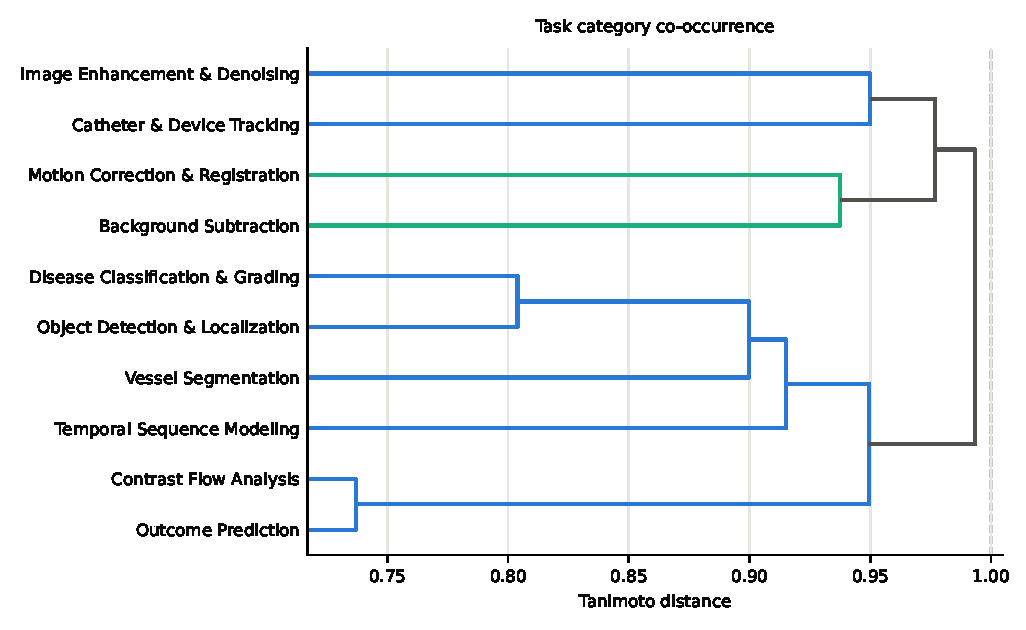
\includegraphics[width=1\linewidth, height=10cm]{figs/task_dendrogram.pdf}
\caption{Average-linkage clustering of ten computational task categories using Tanimoto distances between their study-membership sets, including primary and secondary task assignments. Merges further left indicate greater overlap. All merge distances fall between \edit{0.74} and 1.00; the axis is restricted to this range, and the two sub-clusters with the lowest merge distances are highlighted in color.}
\label{fig:task_dendrogram}
\end{figure*}




\subsubsection{Temporal Modeling}
\label{subsec:temporal_taxonomy}

This subsection examines \edit{how studies use information across frames}. We categorized temporal modeling strategies and compared their use across tasks, imaging modalities, anatomical regions, and publication periods. Table~\ref{tab:temporal_taxonomy} summarizes these strategies and Table~\ref{tab:temporal_crosstab} shows their distribution across study characteristics.

\edit{Ninety-five} of the \edit{115} studies \edit{(82.6\%)} explicitly consider sequential data (linked frames, where a particular visual data instance contains a set of image frames), \edit{and} \edit{20 (17.4\%)} process frames \edit{independently.} \edit{This high proportion partly reflects inclusion criterion I2. The most common} strategies are 3D/video convolution \edit{and} optical flow or registration \edit{(19} \edit{studies each), followed by} recurrent networks \edit{and} frame aggregation \edit{(16 each)} and hemodynamic or physics-based models \edit{(15).} Transformer or state-space models are least common (10 studies, \edit{8.7\%),} all published from 2023 onward. \edit{Frame aggregation is a boundary case: a 2D network trained on stacked frames can learn short-range relations between them, but the sequence has no dedicated temporal mechanism.}

Temporal modeling varies by task, from 100\% for temporal sequence modeling \edit{and contrast flow analysis} to 67\% for catheter and device tracking, Table~\ref{tab:temporal_crosstab}. It is slightly more common in DSA studies \edit{(87\%)} than in X-ray/fluoroscopy studies \edit{(80\%),} and in neurologic studies \edit{(91\%)} than in cardiac \edit{(79\%)} or abdominopelvic studies (60\%). Its prevalence increased substantially over the study period from 40\% in 2018--2019 (2 of 5 studies) to 75--100\% in 2020--2025. In the partial year 2026, it fell to \edit{59\%} (10 of \edit{17} studies).

Of the 95 studies that use sequential frame data, 50 use fixed operations, namely frame aggregation, optical flow or registration, and hemodynamic models. The remaining \edit{45} \edit{(39.1\%} of all studies) learn temporal representations through recurrent, 3D/video, or transformer/state-space models. Learned temporal models are concentrated in disease classification \edit{(20} of \edit{29} studies), absent from image enhancement and device tracking (0 of 9 each), and uncommon in flow analysis \edit{(1 of 8)} and outcome prediction (1 of \edit{9).} Their prevalence increased from \edit{28.2\%} in 2018--2022 \edit{(11} of \edit{39} studies) to \edit{44.7\%} in 2023--2026 \edit{(34} of \edit{76).} Nevertheless, 41 studies \edit{(35.7\%)} use short frame stacks rather than full sequences, and \edit{61 of all 115 studies} identify limited temporal modeling as a limitation.

\vspace{0.25cm}
\begin{mdframed}[linewidth=0.5pt, linecolor=black, backgroundcolor=blue!10]
\textbf{Finding 3.} Although \edit{82.6\%} of studies used sequential frame data, roughly half use fixed temporal operations. Learned temporal representations remain concentrated in classification, while transformer or state-space models appear in only \edit{8.7\%} of studies.
\end{mdframed}
\vspace{0.25cm}





\subsection{Publication Venues}
\label{subsec:venues}

This subsection examines the venues in which the included studies were published. Publication venues indicate which research communities contribute to the field and which journals and proceedings readers need to follow to keep up with it. Figure~\ref{fig:venue_stacked} shows the most frequent venues, while Figure~\ref{fig:venue_curve} shows the cumulative share of studies as venues are added in descending order of publication count.

Of the \edit{115} included studies, \edit{86} \edit{(74.8\%)} were journal articles, \edit{22} \edit{(19.1\%)} were conference papers, and 7 \edit{(6.1\%)} were preprints. Figure~\ref{fig:venue_stacked} shows that the SPIE proceedings are the most frequent outlet, with \edit{10} \edit{studies.} IJCARS and IEEE TMI follow with 5 studies each, and Medical Image Analysis with 4. IEEE venues \edit{and SPIE proceedings each account for 10 studies,} while MICCAI accounts for 3.


% None of the articles appeared in ACM venues; because ACM is a major computing publisher, this suggests that the work is published in imaging and medical venues rather than in general computer-science outlets.

Figure~\ref{fig:venue_curve} \edit{shows how widely the studies are spread across venues.} The \edit{17} most frequent venues account for \edit{half} of the \edit{studies,} \edit{and 50} venues are required to reach 80\%. Of the \edit{72} venues, \edit{54} contribute only one study.

\vspace{0.25cm}
\begin{mdframed}[linewidth=0.5pt, linecolor=black, backgroundcolor=blue!10]
\textbf{Finding 4.} The selected \edit{115} publications are dispersed across \edit{72} venues, \edit{54} of which contribute a single study. Because no venue concentrates this literature, researchers and practitioners seeking to understand the current state of the field must survey a broad range of journals and conference proceedings.
\end{mdframed}
\vspace{0.25cm}

% Figures 7 and 8 share one full-width float so they do not leave half-empty column pages;
% width= sets the cas-dc caption width for each side.
\begin{figure*}[pos=!tp,width=\columnwidth]
\begin{minipage}[t]{\columnwidth}
\centering
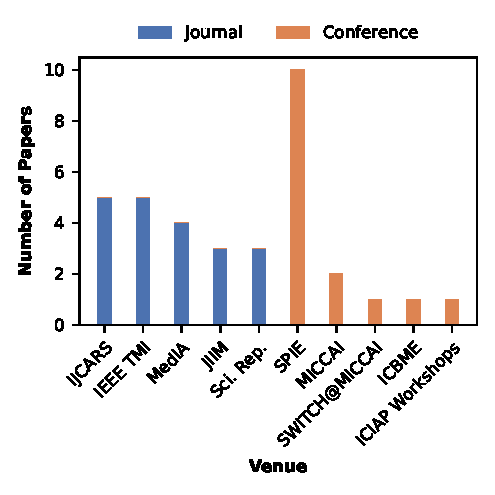
\includegraphics[width=\linewidth]{figs/venue_analysis_stacked.pdf}
\caption{Top publication venues by study count, stratified by venue type. IJCARS: International Journal of Computer Assisted Radiology and Surgery; IEEE TMI: IEEE Transactions on Medical Imaging; MedIA: Medical Image Analysis; JIIM: Journal of Imaging Informatics in Medicine; Sci.\ Rep.: Scientific Reports; SPIE: Proceedings of SPIE; MICCAI: International Conference on Medical Image Computing and Computer-Assisted Intervention; SWITCH@MICCAI: SWITCH workshop at MICCAI; ICBME: Iranian Conference on Biomedical Engineering; \edit{ICIAP} \edit{Workshops: workshops} of the \edit{International} \edit{Conference} \edit{on} \edit{Image} \edit{Analysis} \edit{and} Processing.}
\label{fig:venue_stacked}
\end{minipage}\hfill
\begin{minipage}[t]{\columnwidth}
\centering
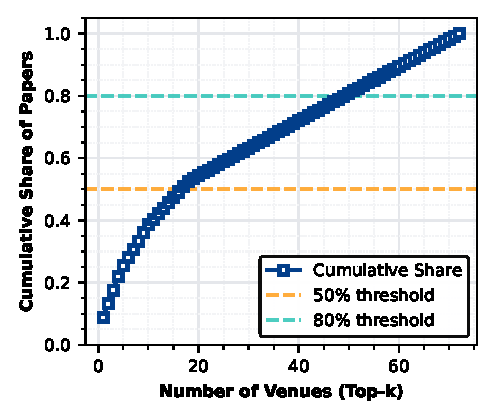
\includegraphics[width=\linewidth]{figs/venue_cumulative_curve.pdf}
\caption{Cumulative share of the \edit{115 studies (one without a stated venue)} across \edit{72} venues, ranked by study count. Dashed lines mark 50\% (yellow) and 80\% (green).}
\label{fig:venue_curve}
\end{minipage}
\end{figure*}


\subsection{Reported Performance}
\label{subsec:performance}

Reported performance metrics are the main basis on which studies compare methods, but each value is meaningful only together with the dataset, validation design, and metric definition that produced it. This subsection examines the reported performance values and their variation across metric families. The values are grouped by metric family and their distributions are shown as a histogram on a scale of 0--100 in Figure~\ref{fig:metric_histogram}. These summaries describe reported results rather than pooled estimates of model performance.

Figure~\ref{fig:metric_histogram} \edit{shows that, within each metric family,} reported scores are concentrated near the upper end of the \edit{scale,} although several studies report substantially lower values. \edit{Taking each study's primary metric, accuracy is reported by 26 studies (mean 86.6, SD 12.0), AUC by 24 (mean 85.7, SD 8.6), Dice/F1 by 14 (mean 87.9, SD 7.5)} and detection precision/recall \edit{by} \edit{10} \edit{(mean} \edit{89.9,} \edit{SD} \edit{12.5);} \edit{IoU} is reported by a single study (75.4). \edit{These families measure different quantities, so we did not average across them.} 

Nonetheless, heterogeneity in datasets, evaluation protocols, and metric definitions precluded direct comparison of performance across studies, and few studies shared a common dataset. A quantitative meta-analysis of reported results was therefore not conducted. Grouping metrics into families does not make them interchangeable, and accuracy alone can obscure poor performance on minority classes. The concentration of high values may reflect selective reporting or testing on data similar to the training data. However, this distribution analysis alone cannot establish either explanation.

\vspace{0.25cm}
\begin{mdframed}[linewidth=0.5pt, linecolor=black, backgroundcolor=blue!10]
\textbf{Finding 5.} Reported performance is generally high, but differences in datasets, protocols, and metrics prevent reliable cross-study rankings in the absence of a shared benchmark.
\end{mdframed}
\vspace{0.25cm}




\begin{figure*}[pos=!tp]
\centering
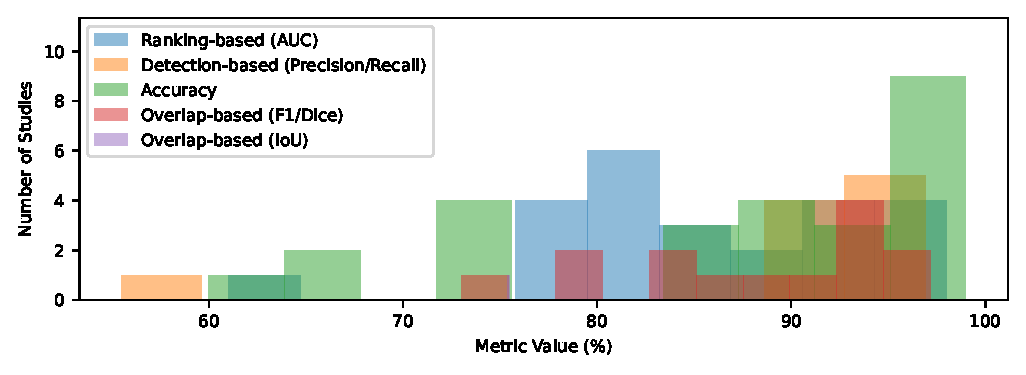
\includegraphics[width=1\linewidth]{figs/histogram_metrics.pdf}
\caption{Distributions of reported performance values by metric family, expressed on a 0--100 scale. Values are descriptive and do not represent pooled performance estimates.}
\label{fig:metric_histogram}
\end{figure*}


% Figure~\ref{fig:metric_kde} provides a smoothed view of these distributions, making their concentration and spread easier to distinguish.

% \begin{figure}[!htbp]
% \centering
% 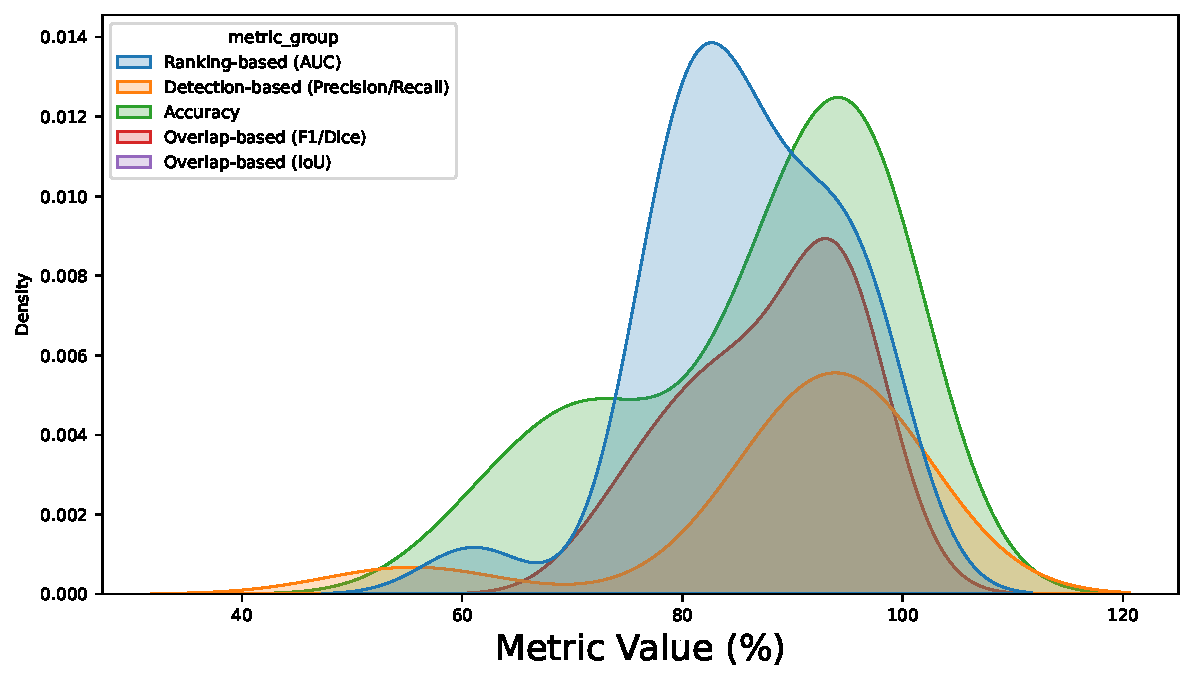
\includegraphics[width=1\linewidth]{figs/kde_metrics.pdf}
% \caption{Kernel density estimates showing smoothed distributions of reported performance values by metric family. Differences in study settings and metric definitions limit direct comparisons.}
% \label{fig:metric_kde}
% \end{figure}




\subsection{Reporting Quality and Clinical Readiness}
\label{subsec:reporting_quality}

We assessed reporting completeness against the 44 items of the CLAIM 2024 checklist~\cite{Tejani2024}, using its official item numbers, and separately summarized evidence supporting clinical \edit{use.} Items are summarized within the 14 subsections of the checklist, from Title and abstract (items 1--2) to Other information (items 42--44), and we compared studies published up to 2024 with those published from 2025 onward as an early check of whether the most recent literature shows any shift toward the updated checklist.


\definecolor{claimTA}{HTML}{4C72B0}
\definecolor{claimIntro}{HTML}{55A868}
\definecolor{claimMeth}{HTML}{C44E52}
\definecolor{claimRes}{HTML}{DD8452}
\definecolor{claimDisc}{HTML}{8172B2}
\definecolor{claimRepro}{HTML}{937860}

\begin{table*}[pos=!tp]
  \centering
  \caption{Reporting completeness by CLAIM 2024 checklist subsection, studies published up to 2024 vs.\ from 2025 onward. The split follows the publication of CLAIM 2024~\cite{Tejani2024}. Items are official CLAIM 2024 item numbers with short descriptions.}
  \label{tab:claim2024_temporal}

  \footnotesize
  \renewcommand{\arraystretch}{1.25}
  \setlength{\tabcolsep}{4pt}

  \resizebox{\textwidth}{!}{%
  \begin{tabular}{@{}
      p{2.6cm}
      c
      p{8.6cm}
      r r
      r r
      >{\centering\arraybackslash}p{1.9cm}
  @{}}

    \toprule

    \multicolumn{1}{l}{\textbf{Subsection}} &
    \multicolumn{1}{c}{\textbf{Items}} &
    \multicolumn{1}{l}{\textbf{CLAIM 2024 checklist items}} &
    \multicolumn{2}{c}{$\boldsymbol{\leq 2024}$ \textbf{(N\,=\,\edit{73})}} &
    \multicolumn{2}{c}{$\boldsymbol{\geq 2025}$ \textbf{(N\,=\,\edit{42})}} &
    \multicolumn{1}{c}{$\boldsymbol{\Delta}$ \textbf{($p$)}} \\

    \cmidrule(lr){4-5}
    \cmidrule(lr){6-7}

    & & &
    \textbf{\%} & \textbf{95\% CI} &
    \textbf{\%} & \textbf{95\% CI} &
    \\

    \midrule

    \rowcolor{claimTA!15}
    \multicolumn{8}{l}{\textbf{\textcolor{claimTA}{Title/Abstract}}} \\

    Title \& abstract & 1--2 & 1 identification as an AI study; 2 structured summary of design, methods, results and conclusions
    & 100\% & [95, 100]
    & 100\% & [92, 100]
    & $\pm0\%$ (1.00) \\

    \midrule
    \rowcolor{claimIntro!15}
    \multicolumn{8}{l}{\textbf{\textcolor{claimIntro}{Introduction}}} \\

     & 3--4 & 3 scientific and clinical background, including the intended role of AI; 4 aims and objectives
    & 100\% & [95, 100]
    & 100\% & [92, 100]
    & $\pm0\%$ (1.00) \\

    \midrule
    \rowcolor{claimMeth!15}
    \multicolumn{8}{l}{\textbf{\textcolor{claimMeth}{Methods}}} \\

    Study design & 5--6 & 5 prospective or retrospective; 6 study goal and intended use
    & 100\% & [95, 100]
    & 100\% & [92, 100]
    & $\pm0\%$ (1.00) \\

    Data & 7--13 & 7 data sources; 8 inclusion and exclusion criteria; 9 data preprocessing; 10 selection of data subsets; 11 de-identification; 12 missing data; 13 image acquisition protocol
    & \edit{59\%} & [47, \edit{70]}
    & \edit{64\%} & \edit{[49,} \edit{77]}
    & $+5\%$ \edit{(0.69)} \\

    Reference standard & 14--18 & 14 definition of the reference standard; 15 rationale for choosing it; 16 source of annotations and annotator qualifications; 17 annotation of the test set; 18 inter- and intrarater variability
    & 76\% & [65, \edit{85]}
    & \edit{69\%} & \edit{[54,} \edit{81]}
    & $-7\%$ \edit{(0.51)} \\

    Data partitions & 19--20 & 19 assignment of data to partitions; 20 level at which partitions are disjoint
    & 84\% & \edit{[74,} \edit{91]}
    & \edit{78\%} & \edit{[63,} \edit{88]}
    & $-6\%$ \edit{(0.45)} \\

    Testing data & 21 & 21 intended sample size
    & 4\% & [1, \edit{12]}
    & 5\% & [1, 16]
    & $+1\%$ (1.00) \\

    Model & 22--24 & 22 detailed model description; 23 software libraries and frameworks; 24 initialization of model parameters
    & \edit{67\%} & \edit{[56,} \edit{77]}
    & \edit{64\%} & \edit{[49,} \edit{77]}
    & $-3\%$ (0.84) \\

    Training & 25--27 & 25 training details (augmentation, objective function, hyperparameters, stopping criteria); 26 selection of the final model; 27 ensembling
    & \edit{54\%} & [42, \edit{65]}
    & \edit{44\%} & \edit{[30,} \edit{59]}
    & $-10\%$ \edit{(0.43)} \\

    Evaluation & 28--34 & 28 performance metrics and comparison with prior models; 29 statistical significance and uncertainty; 30 robustness or sensitivity analysis; 31 explainability; 32 evaluation on internal data; 33 testing on external data; 34 clinical trial registration
    & \edit{59\%} & [47, \edit{70]}
    & \edit{60\%} & \edit{[45,} \edit{73]}
    & \edit{$+1\%$} (1.00) \\

    \midrule
    \rowcolor{claimRes!15}
    \multicolumn{8}{l}{\textbf{\textcolor{claimRes}{Results}}} \\

    Data & 35--36 & 35 numbers of patients or examinations included and excluded; 36 demographic and clinical characteristics
    & \edit{54\%} & \edit{[43,} \edit{65]}
    & \edit{64\%} & \edit{[49,} \edit{77]}
    & $+10\%$ \edit{(0.33)} \\

    Model performance & 37--39 & 37 performance on all partitions and datasets; 38 diagnostic performance estimates with their precision; 39 failure analysis
    & \edit{92\%} & \edit{[83,} 96]
    & \edit{81\%} & \edit{[67,} \edit{90]}
    & $-11\%$ \edit{(0.14)} \\

    \midrule
    \rowcolor{claimDisc!15}
    \multicolumn{8}{l}{\textbf{\textcolor{claimDisc}{Discussion}}} \\

     & 40--41 & 40 limitations; 41 implications for practice
    & 100\% & [95, 100]
    & \edit{98\%} & \edit{[88,} \edit{100]}
    & $-2\%$ \edit{(0.37)} \\

    \midrule
    \rowcolor{claimRepro!15}
    \multicolumn{8}{l}{\textbf{\textcolor{claimRepro}{Other information}}} \\

     & 42--44 & 42 reference to the full protocol or technical details; 43 availability of software, model or data; 44 funding and role of funders
    & \edit{51\%} & \edit{[40,} \edit{62]}
    & \edit{71\%} & \edit{[56,} \edit{83]}
    & $+21\%$ \edit{(0.03)} \\

    \bottomrule

  \end{tabular}%
  }

  \par\smallskip
  \footnotesize
  \textit{Note:} Proportion of studies in which the subsection is reported (at least half of its applicable items), among studies where it applies, with 95\% Wilson CIs. $\Delta$: difference from unrounded proportions, with the two-sided Fisher's exact $p$-value. No subsection is significant after Holm correction (smallest adjusted \edit{$p=0.46$}). Item 34 (clinical trial registration) was not applicable to any study.

\end{table*}
% \definecolor{claimTA}{HTML}{4C72B0}
% \definecolor{claimIntro}{HTML}{55A868}
% \definecolor{claimMeth}{HTML}{C44E52}
% \definecolor{claimRes}{HTML}{DD8452}
% \definecolor{claimDisc}{HTML}{8172B2}
% \definecolor{claimRepro}{HTML}{937860}

% \begin{table}[ht]
%   \centering
%   \caption{CLAIM 2024 Adherence by Thematic Cluster: Temporal Comparison
%     ($\leq 2024$ vs.\ $\geq 2025$).}
%   \label{tab:claim2024_temporal}

%   \footnotesize
%   \renewcommand{\arraystretch}{1.25}
%   \setlength{\tabcolsep}{4pt}

%   \resizebox{\columnwidth}{!}{%
%   \begin{tabular}{@{}
%       l
%       p{6.2cm}
%       r r
%       r r
%       >{\centering\arraybackslash}p{1.2cm}
%   @{}}

%     \toprule

%     \multicolumn{1}{l}{\textbf{ID}} &
%     \multicolumn{1}{l}{\textbf{Cluster}} &
%     \multicolumn{2}{c}{$\boldsymbol{\leq 2024}$ \textbf{(N\,=\,77)}} &
%     \multicolumn{2}{c}{$\boldsymbol{\geq 2025}$ \textbf{(N\,=\,43)}} &
%     \multicolumn{1}{c}{$\boldsymbol{\Delta}$} \\

%     \cmidrule(lr){3-4}
%     \cmidrule(lr){5-6}

%     & &
%     \textbf{\%} & \textbf{95\% CI} &
%     \textbf{\%} & \textbf{95\% CI} &
%     \\

%     \midrule

%     \rowcolor{claimTA!15}
%     \multicolumn{7}{l}{\textbf{\textcolor{claimTA}{Title/Abstract}}} \\

%     C01 & AI identification \& abstract completeness
%     & 71\% & [62, 78]
%     & 75\% & [62, 84]
%     & $+4\%$~$\uparrow$ \\

%     \midrule

%     \rowcolor{claimIntro!15}
%     \multicolumn{7}{l}{\textbf{\textcolor{claimIntro}{Introduction}}} \\

%     C02 & Background \& study objectives
%     & 98\% & [94, 100]
%     & 98\% & [91, 100]
%     & $\pm0\%$~$\sim$ \\

%     \midrule

%     \rowcolor{claimMeth!15}
%     \multicolumn{7}{l}{\textbf{\textcolor{claimMeth}{Methods}}} \\

%     C03 & Study design \& data sources
%     & 42\% & [34, 50]
%     & 61\% & [48, 72]
%     & $+19\%$~$\uparrow$ \\

%     C04 & Participants \& image acquisition
%     & 29\% & [21, 37]
%     & 38\% & [26, 51]
%     & $+9\%$~$\uparrow$ \\

%     C05 & Reference standards \& annotation
%     & 31\% & [24, 40]
%     & 46\% & [34, 59]
%     & $+15\%$~$\uparrow$ \\

%     C06 & Data partitioning \& class handling
%     & 44\% & [36, 53]
%     & 44\% & [31, 57]
%     & $\pm0\%$~$\sim$ \\

%     C07 & Model architecture \& training
%     & 65\% & [56, 72]
%     & 64\% & [50, 75]
%     & $-1\%$~$\sim$ \\

%     C08 & Evaluation design \& interpretability
%     & 24\% & [17, 32]
%     & 52\% & [39, 64]
%     & $+28\%$~$\uparrow$ \\

%     \midrule

%     \rowcolor{claimRes!15}
%     \multicolumn{7}{l}{\textbf{\textcolor{claimRes}{Results}}} \\

%     C09 & Performance \& external validation
%     & 35\% & [27, 44]
%     & 44\% & [31, 57]
%     & $+9\%$~$\uparrow$ \\

%     C10 & Demographic \& subgroup reporting
%     & 8\% & [4, 14]
%     & 16\% & [9, 28]
%     & $+8\%$~$\uparrow$ \\

%     \midrule

%     \rowcolor{claimDisc!15}
%     \multicolumn{7}{l}{\textbf{\textcolor{claimDisc}{Discussion}}} \\

%     C11 & Limitations, implications \& supporting documentation
%     & 84\% & [77, 90]
%     & 89\% & [79, 95]
%     & $+5\%$~$\uparrow$ \\

%     \midrule

%     \rowcolor{claimRepro!15}
%     \multicolumn{7}{l}{\textbf{\textcolor{claimRepro}{Reproducibility \& Transparency}}} \\

%     C12 & Reproducibility \& funding disclosure
%     & 21\% & [15, 29]
%     & 23\% & [14, 36]
%     & $+2\%$~$\sim$ \\

%     \bottomrule

%     \multicolumn{7}{p{\hsize}}{%
%       \textit{Note:} Proportions are the fraction of studies reporting adherence
%       (``Yes'') among those where the item was applicable (NA excluded).
%       95\% Wilson confidence intervals are shown.
%       $\Delta$ = post--pre difference; arrows indicate changes greater than
%       2 percentage points.
%     } \\

%   \end{tabular}%
%   }

% \end{table}


Table~\ref{tab:claim2024_temporal} shows reporting completeness for each checklist subsection with 95\% Wilson confidence intervals and the comparisons between publication periods. The title, abstract, introduction and study design subsections are reported by every study, and the discussion by nearly all. Methods reporting is weaker and less consistent: training details (items 25--27) are reported by \edit{54\%} and \edit{44\%} of studies in the two periods, and the testing-data subsection (item 21, intended sample size) by only 4\% and 5\%. The largest differences between periods are in other information (items 42--44: \edit{51\%} to \edit{71\%,} unadjusted \edit{$p=0.03$}), model performance (items 37--39: \edit{92\%} to \edit{81\%,} $p=0.14$) and results data (items 35--36: \edit{54\%} to \edit{64\%,} $p=0.33$). No difference is statistically significant after Holm correction (smallest adjusted \edit{$p=0.46$}).

\edit{At the item level, reporting rates were calculated across all 115 studies, with nonapplicable items counted as not reported. Test-set size justification was the least reported item (item 21: 5 studies, 4.3\%), followed by external testing (item 33: 19, 16.5\%) and inter-rater variability (item 18: 23, 20.0\%). Other infrequently reported items were explainability (item 31: 26, 22.6\%), de-identification (item 11: 27, 23.5\%), complete training details (item 25: 29, 25.2\%), statistical uncertainty (item 29: 30, 26.1\%) and handling of missing data (item 12: 31, 27.0\%). Demographic and clinical characteristics were reported by 48 studies (item 36: 41.7\%). Low reporting rates across all studies sometimes reflected limited applicability: ensembling (item 27) was reported by 10 of the 11 studies that used ensembles. Trial registration (item 34) did not apply to any study because none was a clinical trial.}




Although 52 studies \edit{(45.2\%)} include a statement on the availability of software, models or data (item 43), only 25 studies \edit{(21.7\%)} publicly release code and 3 \edit{(2.6\%)} publicly release their own data. We counted a release only when the article gave a working repository or archive link; statements that data are available on reasonable request, made by \edit{26} further studies, were not counted. An availability statement does not necessarily indicate public release, because many such statements restrict access. Evidence supporting clinical use was also limited: 19 studies \edit{(16.5\%)} report external validation, including one that also reports prospective deployment; 3 \edit{(2.6\%)} use a prospective design; 4 \edit{(3.5\%)} report clinical deployment or live use; and 4 \edit{(3.5\%)} discuss regulatory requirements. These categories are not mutually exclusive.

\vspace{0.25cm}
\begin{mdframed}[linewidth=0.5pt, linecolor=black, backgroundcolor=blue!10]
\textbf{Finding 6.} Against the CLAIM 2024 checklist, title, abstract, introduction and study design are well reported, but test-set size justification, external testing, inter-rater variability, training details, statistical uncertainty, demographic characteristics, code and data sharing, and evidence of clinical use remain limited. We found no statistically significant difference in reporting in studies published prior to, and after, the CLAIM-2024 publication.
\end{mdframed}
\vspace{0.25cm}


\subsection{Research Gaps}
\label{sec:research_gaps}

\begin{figure*}[pos=htbp]
  \centering
  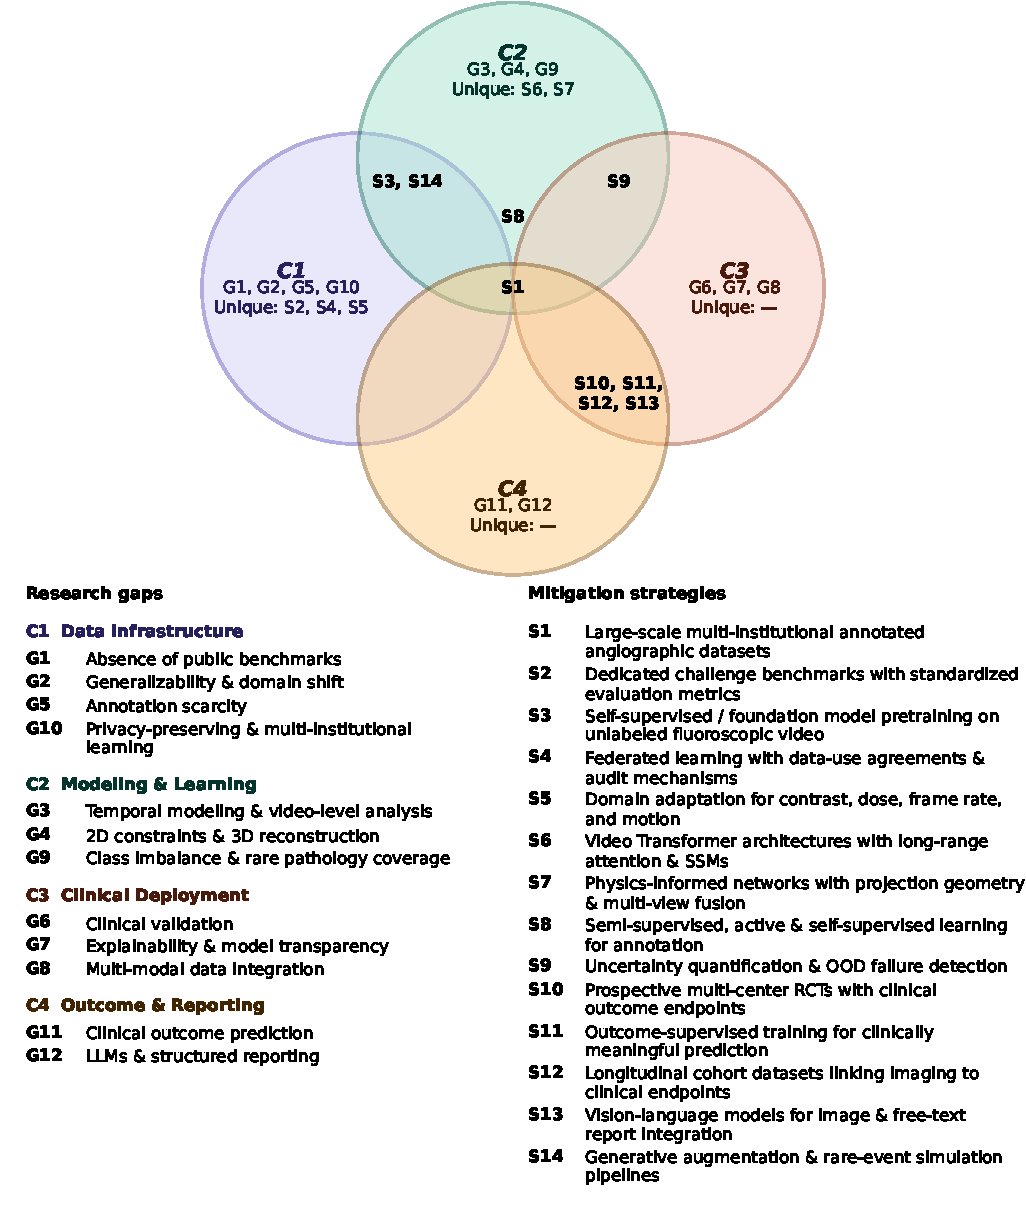
\includegraphics[width=0.9\textwidth]{figs/venn_diagram.pdf}
  \caption{Research gaps grouped into four clusters, with mitigation strategies. C1: Data Infrastructure (G1, G2, G5, G10); C2: Modeling \& Learning (G3, G4, G9); C3: Clinical Deployment (G6, G7, G8); C4: Outcome \& Reporting (G11, G12). Strategy codes (S1--S14, defined in the legend) sit in the clusters or overlaps they serve; \edit{unlabeled} overlaps have no shared strategy. Gap codes follow Table~\ref{tab:research_gaps}.}
  \label{fig:venn_gaps}
\end{figure*}

We identified twelve research gaps (G1--G12) and organized them into four clusters (C1--C4), which are shown in Figure~\ref{fig:venn_gaps}. \textit{Data Infrastructure} (C1: G1, G2, G5, G10) includes dataset size and availability, generalization across sites, annotation scarcity, and privacy-preserving learning. \textit{Modeling \& Learning} (C2: G3, G4, G9) includes limited temporal modeling, reliance on 2D projections, and class imbalance. \textit{Clinical Deployment} (C3: G6, G7, G8) addresses gaps in prospective validation, explainability, and multimodal integration. \textit{Outcome \& Reporting} (C4: G11, G12) addresses the connection between image-level performance and clinical outcomes, along with structured reporting.

Figure~\ref{fig:venn_gaps} also shows how proposed strategies address gaps across multiple clusters. Large annotated datasets (S1) support all four clusters. Pretraining on unlabeled video (S3) and generative augmentation (S14) connect data infrastructure with modeling, while annotation-efficient learning (S8) also supports clinical deployment. Uncertainty quantification (S9) connects modeling with deployment. Prospective trials, outcome-supervised training, longitudinal cohorts, and vision--language models (S10--S13) connect clinical deployment with outcomes and reporting. Table~\ref{tab:research_gaps} presents the evidence for each gap and the corresponding strategies.

% Table 6 is split into full-width floats (four gaps each) so it flows with
% the two-column text instead of forcing a one-column page break.
\begin{table*}[pos=!t]
\caption{Research gaps, supporting evidence from the included studies, and mitigation strategies. Cluster codes C1--C4 follow Figure~\ref{fig:venn_gaps}.}
\label{tab:research_gaps}
\footnotesize
\begin{tabular}{>{\raggedright\arraybackslash}p{2.5cm}
                  >{\raggedright\arraybackslash}p{6.2cm}
                  >{\raggedright\arraybackslash}p{6.2cm}}
\toprule
\textbf{Research Gaps} & \textbf{Evidence from the Literature} &
\textbf{Mitigation Strategies} \\
\midrule
\textbf{G1:} Absence of Public Benchmarks\newline\textit{C1}
&
\tabitem Small, private, single-center datasets dominate; \edit{42} of the \edit{91} studies that report patient numbers include fewer than 200 patients \cite{ref20,R1609,R1362,R1674,R1680,ref93}.\newline
\tabitem Public, annotated datasets are lacking for many angiographic tasks, devices and territories; only 20 of \edit{115} studies use a public dataset and 3 release their own data \cite{ref178,ref35,ref36,ref67,ref97,ref162}.\newline
\tabitem Absence of shared benchmarks makes cross-study comparison practically impossible \cite{R0100,ref43,ref48,ref92,ref94,ref95}.\newline
\tabitem Inconsistent evaluation protocols prevent measurement of field-wide progress \cite{R2411,ref100}.
&
\tabitem Construct and release large-scale multi-institutional angiographic datasets with standardized annotations and defined train/test splits \cite{R0099,ref35,ref97}.\newline
\tabitem Organize dedicated challenge benchmarks modeled on established algorithmic medical image interpretation competitions, building on the public datasets already reused by included studies \cite{ref15,ref211,ref64,R1222,ref48,R0099}.\newline
\tabitem Mandate inter-rater reliability protocols in annotation guidelines to ensure label quality \cite{R1213}.\newline
\tabitem Construct longitudinal multi-modal cohort datasets linking angiographic sequences to post-procedural outcomes \cite{R0643,ref76}.\newline
% \tabitem Define standard evaluation metrics and phantom-versus-patient evaluation subsets \cite{R0058}.
\\
\dashedrule
\textbf{G2:} Generalizability \& Domain Shift\newline\textit{C1}
&
\tabitem \edit{Most models are} trained \edit{and tested} on \edit{data from} a single vendor or acquisition \edit{protocol,} \edit{and} \edit{their} \edit{authors note that} transfer to external settings \edit{is untested} \cite{ref91,ref178,ref38,ref56,ref93,ref99}.\newline
\tabitem Domain shift between synthetic training data and real clinical images remains unresolved \cite{R1565,ref43,ref52,ref67,ref74,R3910}.\newline
\tabitem Methods \edit{are} \edit{typically} \edit{developed} \edit{within} \edit{one} \edit{vascular} \edit{territory} or \edit{view,} \edit{and their authors list performance in other territories or lesion types as unknown} \cite{ref208,R4204,R4557,ref179}.\newline
\tabitem Multi-center heterogeneity in frame rate, contrast dosing, and radiation settings is rarely addressed \cite{ref42,R3093,R1680,ref92}.
&
\tabitem Treat external multi-institutional validation as a prerequisite for clinical deployment across institutions \cite{ref198,R2873,ref65,ref94,ref152,ref155}.\newline
\tabitem Develop domain adaptation methods tailored to variable contrast concentration, dose, frame rate, and motion profiles \cite{ref64}.\newline
\tabitem Extend personalized federated learning frameworks to accommodate non-identical cross-center data distributions \cite{R2443}.\newline
\tabitem Establish domain shift benchmarks to quantify performance degradation across different imaging vendors \cite{ref65,ref99,R3338}.
\\
\dashedrule
\textbf{G3:} Temporal Modeling \& Video-Level Analysis\newline\textit{C2}
&
\tabitem Temporal information is often modeled only superficially: \edit{20} of \edit{115} studies process each frame independently, and half of the \edit{95} temporally aware studies rely on fixed operations rather than learned temporal representations of flow and contrast propagation \cite{ref64,ref15,R1541,ref50,ref82,ref10}.\newline
\tabitem Temporal models are typically restricted to short fixed-length clips, not full variable-length sequences \cite{R1222,R3149,R3712}.\newline
\tabitem Procedural phase transitions during interventional procedures are not explicitly modeled \cite{R3129,R4208,ref94,R2443}.\newline
\tabitem Respiratory and cardiac motion are treated as noise rather than informative temporal signals \cite{ref36,R4220,ref34}.
&
\tabitem Develop architectures that model the complete temporal structure of angiographic acquisitions, including mask, injection, and washout phases \cite{R1939,ref46,R1609}.\newline
\tabitem Evaluate video Transformer architectures with long-range attention and state-space models for efficient long-sequence processing \cite{ref42,R1222,ref104}.\newline
\tabitem Explore temporal self-supervised pretraining on large archives of unannotated fluoroscopic video \cite{R2400,ref39}.\newline
\tabitem Incorporate explicit hemodynamic priors, such as contrast agent kinetics, into temporal model design \cite{ref43,ref46}.
\\
\dashedrule
\textbf{G4:} 2D Constraints \& 3D Reconstruction\newline\textit{C2}
&
\tabitem Angiographic projections collapse 3D vascular anatomy, introducing foreshortening, vessel overlap, and depth loss \cite{R1263,R1503,R1565,ref60,ref97,ref35}.\newline
\tabitem The vast majority of methods operate exclusively on single-plane 2D projections \cite{R3129,ref148,ref43,ref78,R4557}.\newline
\tabitem Accurate 3D reconstruction from monoplane or biplane projections under intraoperative time constraints remains unsolved \cite{R3164,R2466,ref46,ref96}.\newline
\tabitem 2D/3D registration accuracy is insufficient for routine intraoperative use \cite{ref40,R3910,ref99,ref92}.
&
\tabitem Develop multi-view learning architectures that fuse information across projection angles \cite{ref148,R4557,ref35,R2466}.\newline
\tabitem Investigate physics-informed networks incorporating known projection geometry \cite{ref43,R3164}.\newline
\tabitem Use rotational angiographic acquisitions for temporally informed 3D reconstruction \cite{ref152,R3338}.\newline
\tabitem Systematically combine intra-procedural cone-beam CT with fluoroscopic AI pipelines to provide 3D context \cite{R2466,R3164,ref39}.
\\
\bottomrule
\end{tabular}
\end{table*}

\begin{table*}[pos=!t]
{\sffamily\small\textbf{\color{scolor}\tablename~\ref*{tab:research_gaps}} (continued)\par}\vskip4pt
\footnotesize
\begin{tabular}{>{\raggedright\arraybackslash}p{2.5cm}
                  >{\raggedright\arraybackslash}p{6.2cm}
                  >{\raggedright\arraybackslash}p{6.2cm}}
\toprule
\textbf{Research Gaps} & \textbf{Evidence from the Literature} &
\textbf{Mitigation Strategies} \\
\midrule
\textbf{G5:} Annotation Scarcity \& Annotation-Efficient Learning\newline\textit{C1}
&
\tabitem Manual data annotation \edit{takes a large amount of physician time} and specialist expertise for every labeled study \cite{R0521,ref34,ref56,R4204,R4208,ref162}.\newline
\tabitem Annotation varies within and between observers, rarely quantified in included studies \cite{ref28,R1213,ref208,R1674,ref75,R3661}.\newline
\tabitem Synthetic data generation partially addresses scarcity, but synthetic-to-real domain gaps persist \cite{ref64,ref52,ref74}.\newline
\tabitem Semi-supervised and self-supervised methods are underrepresented across angiographic analysis tasks \cite{ref2,ref57,R2411}.
&
\tabitem Systematically evaluate semi-supervised, self-supervised, and active learning strategies with explicit performance-versus-label-count analysis \cite{R2411,ref94,R3164,R2400}.\newline
\tabitem Pursue foundation model pretraining on large archives of unlabeled fluoroscopic video \cite{R2400}.\newline
\tabitem Validate generative data augmentation methods informed by realistic vascular anatomy models and imaging physics \cite{ref64,ref43,R1939}.\newline
\tabitem Develop annotation tools that integrate uncertainty estimation to prioritize the most informative cases for expert labeling \cite{ref84}.
\\
\dashedrule
\textbf{G6:} Prospective Clinical Validation \& Outcome Assessment\newline\textit{C3}
&
\tabitem Among the \edit{59} studies that report their design, \edit{55} are retrospective analyses of previously acquired images \cite{ref42,ref38,R3052,R3093,R3126,ref76}.\newline
\tabitem Prospective validation in live clinical settings is almost entirely absent from the literature \cite{ref102,ref91,R0521,R1362,R1503,ref75}.\newline
\tabitem Retrospective evaluation cannot measure the effect of AI outputs on physician behavior or patient outcomes \cite{R0100,ref208,ref80}.\newline
\tabitem Demonstrated technical performance does not establish clinical value or cost-effectiveness \cite{ref152,ref40,ref82,R3661}.
&
\tabitem Design prospective clinical evaluation frameworks in collaboration between AI researchers and clinicians \cite{ref198,R4557}.\newline
\tabitem Pursue randomized controlled trials comparing outcomes under standard-of-care versus AI-assisted decision-making \cite{ref48}.\newline
\tabitem Engage regulatory bodies to define the evidence standards required for clinical deployment \cite{R1362,ref95,R0570}.\newline
\tabitem Develop AI interface designs that integrate model outputs into existing workflow without adding cognitive burden \cite{R1362,ref198}.
\\
\dashedrule
\textbf{G7:} Explainability \& Model Transparency\newline\textit{C3}
&
\tabitem Most deep learning models lack clinically relevant interpretable justification \cite{ref25,R3164,ref173,ref92}.\newline
\tabitem Existing attention visualization approaches provide limited mechanistic insight \cite{R0643,R3155}.\newline
\tabitem Silent failure modes in out-of-distribution inputs are a particular concern for patient safety \cite{ref161}.\newline
\tabitem Regulatory and clinical trust requirements are not satisfied by aggregate performance metrics alone \cite{R1680,R2400,ref89}.
&
\tabitem Treat uncertainty quantification as a core design requirement, which provides confidence alongside every prediction \cite{ref161,ref46}.\newline
\tabitem Develop failure detection systems that flag out-of-distribution inputs for mandatory human review \cite{ref161}.\newline
\tabitem Design intermediate representations aligned with anatomical and hemodynamic concepts in clinical use \cite{R4204,R0521}.\newline
\tabitem Evaluate whether explainability outputs demonstrably improve clinical decision-making in prospective user studies \cite{R1939}.
\\
\dashedrule
\textbf{G8:} Multi-Modal Data Integration\newline\textit{C3}
&
\tabitem Studies predominantly process angiographic images in isolation, discarding complementary clinical data \cite{ref91,R0643,R1263,ref71}.\newline
\tabitem Pressure wire measurements, IVUS, OCT, CTA, ECG, and laboratory biomarkers are routinely available but unused \cite{ref198,ref25,ref32,R1609,ref46,shi2021temporal}.\newline
\tabitem Missing modalities at inference time, common in clinical practice, are rarely addressed \cite{R2411}.\newline
\tabitem Longitudinal multi-modal datasets linking intraoperative imaging to procedural outcomes are almost absent \cite{ref62,ref30}.
&
\tabitem Develop architectures capable of fusing imaging, hemodynamic, and structured clinical data with explicit handling of missing modalities \cite{ref42,R0643,ref76,ref102}.\newline
\tabitem Explore vision-language model architectures for integrating free-text clinical notes with imaging features \cite{R0643}.\newline
\tabitem Define outcome-oriented multi-modal training objectives that directly target clinical outcomes \cite{ref42,ref127}.
\\
\bottomrule
\end{tabular}
\end{table*}

\begin{table*}[pos=!t]
{\sffamily\small\textbf{\color{scolor}\tablename~\ref*{tab:research_gaps}} (continued)\par}\vskip4pt
\footnotesize
\begin{tabular}{>{\raggedright\arraybackslash}p{2.5cm}
                  >{\raggedright\arraybackslash}p{6.2cm}
                  >{\raggedright\arraybackslash}p{6.2cm}}
\toprule
\textbf{Research Gaps} & \textbf{Evidence from the Literature} &
\textbf{Mitigation Strategies} \\
\midrule
\textbf{G9:} Class Imbalance \& Rare Pathology Coverage\newline\textit{C2}
&
\tabitem Rare events such as vessel perforation, intracranial aneurysm, and gastrointestinal bleeding are severely underrepresented \cite{ref15,R1541,ref60,ref80,ref144,ref227}.\newline
\tabitem Standard training objectives produce models biased toward majority classes with poor sensitivity for critical minority cases \cite{ref161,ref25,ref35,ref48,ref79,ref56}.\newline
\tabitem Rare anatomical variants and complex lesion morphologies are systematically excluded from study cohorts \cite{ref91,R0521,R0570,ref179,ref4,R3155}.\newline
\tabitem Aggregate performance metrics obscure minority-class failure, masking clinically important shortcomings \cite{R0099,ref34,ref89,ref127}.
&
\tabitem Systematically evaluate oversampling, cost-sensitive learning, hard negative mining, and generative augmentation across imbalance ratios \cite{ref46,R3712,ref97,ref162,ref155,ref62}.\newline
\tabitem Explicitly target underrepresented pathology types in dataset construction rather than excluding them \cite{R1541,ref80}.\newline
\tabitem Mandate stratified reporting of performance metrics for rare classes alongside aggregate figures \cite{ref75}.\newline
\tabitem Develop rare-event simulation pipelines for synthetic augmentation of clinically critical minority cases.
\\
\dashedrule
\textbf{G10:} Privacy-Preserving \& Multi-Institutional Learning\newline\textit{C1}
&
\tabitem Patient privacy regulations and data governance barriers prevent centralization of large angiographic datasets \cite{ref52,ref75,ref95,ref162,R0570}.\newline
\tabitem Federated learning for angiographic analysis is barely represented in the reviewed literature; only one study explicitly adopts this framework \cite{R2443}.\newline
\tabitem Non-identical data distributions across institutions complicate federated model training \cite{R2443}.\newline
\tabitem Auditability and accountability requirements for federated clinical AI systems are unaddressed, including by the one federated study \cite{R2443}.
&
\tabitem Develop federated learning frameworks specifically tailored to large angiographic video inputs with efficient communication protocols \cite{R2443}.\newline
\tabitem Evaluate privacy-preserving data-sharing approaches for their impact on model utility \cite{ref46,R2443}.\newline
\tabitem Establish standardized data use agreements and federated audit mechanisms for cross-institutional AI training, since data protection currently limits release or sharing of angiographic datasets \cite{ref75,ref162}.\newline
\tabitem Benchmark personalized federated approaches against centralized baselines as a function of institutional data heterogeneity \cite{R2443}.
\\
\dashedrule
\textbf{G11:} Imaging Biomarkers \& Clinical Outcome Prediction\newline\textit{C4}
&
\tabitem Most methods focus on intermediate imaging tasks rather than on direct clinical outcome prediction \cite{R1680,ref91,ref92}.\newline
\tabitem Demonstrating detection or segmentation accuracy does not establish impact on revascularization decisions or survival \cite{R1362,R1680,ref91}.\newline
\tabitem Longitudinal cohort designs linking imaging findings to follow-up clinical endpoints are largely absent \cite{ref84,R3093,ref89}.\newline
\tabitem Outcome-supervised training objectives have not been systematically explored in the angiographic domain \cite{ref79}.
&
\tabitem Link angiographic archives with procedural databases and electronic health records to build longitudinal datasets with post-procedural endpoints, including re-intervention and mortality \cite{ref42,ref76,ref102,R0643,ref127}.\newline
\tabitem Develop outcome-supervised training objectives that directly target clinical events \cite{R1263,R1609,ref72,R0643}.\newline
\tabitem Apply imaging biomarker discovery workflows combining feature extraction with survival and outcome modeling \cite{R1263,ref76,ref28}.
\\
\dashedrule
\textbf{G12:} Large Language Models \& Structured Reporting\newline\textit{C4}
&
\tabitem Language-model use is almost entirely unexplored; only one included study encodes procedural free-text reports with a pretrained language model, as one input of a mortality-prediction model \cite{R0643}.\newline
\tabitem Free-text angiographic reports contain rich structured information routinely discarded in downstream analyses \cite{R0099,R0521}.\newline
\tabitem That study draws on a cohort from a single country (South Korea) and uses frozen general-purpose encoders rather than models adapted to angiographic reporting \cite{R0643}.\newline
\tabitem Multimodal vision-language models for integrated image-and-report reasoning have not been evaluated in this domain; the only study combining images and reports used frozen general-purpose encoders \cite{R0643}.
&
\tabitem Evaluate open-source LLMs and vision-language models for angiographic report structuring, finding extraction, and downstream decision support \cite{R0643}.\newline
\tabitem Develop end-to-end pipelines that integrate structured imaging outputs with natural language generation for automated report synthesis \cite{R0521,R4204}.\newline
\tabitem Construct standardized angiographic reporting ontologies to provide a shared vocabulary for cross-institutional NLP model training \cite{R0099,ref89}.\newline
\tabitem Benchmark open-source models against proprietary baselines on diverse international angiographic report corpora \cite{R0100}.
\\
\bottomrule
\end{tabular}
\end{table*}



\subsection{Roadmap}
\label{sec:actionable_roadmap}

Table~\ref{tab:cbm_roadmap} turns each gap into a clinical risk, a computational opportunity, and a benchmark that would make progress measurable. Its evidence count is the number of included studies \edit{coded} \edit{as} \edit{documenting} the gap, \edit{that is, studies that state it as a limitation, motivation or direction for future work,} each backed by a verbatim quote. \edit{It counts studies that report the problem, not studies that demonstrate it experimentally; for example, the 67 studies counted for G2 note limited generalizability, but only 12 of them tested a model on external data.} The best-documented gaps are G2, G1 and G3 \edit{(67,} \edit{64} and \edit{61} of \edit{115} studies); G12, G10 and G11 (2, 8 and 9 studies) are emerging directions with limited evidence.

\begin{table*}[pos=!t]
\caption{Roadmap for each research gap: clinical risk, computational opportunity and a benchmark or evaluation recommendation. Evidence count is the number of included studies \edit{coded} \edit{as} \edit{documenting} the \edit{gap (stating it as a limitation, motivation or future work); it does not count studies that demonstrated the gap experimentally.} Cluster codes C1--C4 follow Figure~\ref{fig:venn_gaps}.}
\label{tab:cbm_roadmap}
\footnotesize
\begin{tabular}{>{\raggedright\arraybackslash}p{2.1cm}
                  >{\centering\arraybackslash}p{1.1cm}
                  >{\raggedright\arraybackslash}p{3.95cm}
                  >{\raggedright\arraybackslash}p{3.95cm}
                  >{\raggedright\arraybackslash}p{4.1cm}}
\toprule
\textbf{Gap} & \textbf{Evid.\ Count} & \textbf{Clinical Risk} & \textbf{Computational Opportunity} & \textbf{Benchmark / Evaluation Recommendation} \\
\midrule
\textbf{G1} Absence of Public Benchmarks\newline\textit{C1} & \edit{64} &
Reported performance cannot be verified to generalize beyond the originating institution before deployment, risking undetected failure in new clinical settings. &
Large-scale, standardized, publicly released multi-institutional datasets with defined train/test splits. &
Organize a public challenge benchmark with standardized metrics. \\
\dashedrule
\addlinespace
\textbf{G2} Generalizability \& Domain Shift\newline\textit{C1} & \edit{67} &
Models validated at a single site, vendor, or vascular territory may silently degrade elsewhere, producing unreliable outputs during patient care without warning. &
Domain adaptation and personalized federated learning tailored to cross-vendor, cross-protocol, and cross-territory variation. &
Require external multi-institutional validation and report a domain-shift benchmark quantifying degradation across imaging vendors, imaging protocols, and institutions. \\
\dashedrule
\addlinespace
\textbf{G3} Temporal Modeling \& Video-Level Analysis\newline\textit{C2} & \edit{61} &
Discarding hemodynamic flow and contrast-propagation dynamics risks missing clinically important temporal signals a frame-independent model cannot detect. &
Video-transformer and state-space architectures modeling full acquisition phases (mask, injection, washout) with hemodynamic priors. &
Evaluate on full variable-length real acquisitions with metrics scoring temporal fidelity, not accuracy on short fixed-length clips alone. \\
\dashedrule
\addlinespace
\textbf{G4} 2D Constraints \& 3D Reconstruction\newline\textit{C2} & \edit{46} &
Foreshortening, vessel overlap, and depth loss from monoplane 2D projections can cause missed or mis-measured lesions during intraoperative decisions. &
Multi-view and physics-informed 3D reconstruction from mono-/biplane or rotational angiographic acquisitions. &
Standardized 2D/3D registration accuracy benchmark evaluated under intraoperative time constraints. \\
\dashedrule
\addlinespace
\textbf{G5} Annotation Scarcity \& Annotation-Efficient Learning\newline\textit{C1} & \edit{49} &
Reliance on scarce expert annotation with unquantified inter-observer variability threatens label reliability for safety-critical model training. &
Semi-/self-supervised and active learning, foundation-model pretraining on large archives of unlabeled fluoroscopic video. &
Report performance-versus-label-count curves for each annotation-efficient method, rather than accuracy at a single fixed label budget. \\
\dashedrule
\addlinespace
\textbf{G6} Prospective Clinical Validation \& Outcome Assessment\newline\textit{C3} & 43 &
Because almost no studies validate prospectively, there is no evidence these models change physician behavior or patient outcomes in live care. &
Prospective evaluation frameworks and outcome-supervised training designed jointly with clinicians. &
Randomized controlled trials comparing standard-of-care versus AI-assisted decision-making as the evaluation standard. \\
\dashedrule
\bottomrule
\end{tabular}
\end{table*}

\begin{table*}[pos=!t]
{\sffamily\small\textbf{\color{scolor}\tablename~\ref*{tab:cbm_roadmap}} (continued)\par}\vskip4pt
\footnotesize
\begin{tabular}{>{\raggedright\arraybackslash}p{2.1cm}
                  >{\centering\arraybackslash}p{1.1cm}
                  >{\raggedright\arraybackslash}p{3.95cm}
                  >{\raggedright\arraybackslash}p{3.95cm}
                  >{\raggedright\arraybackslash}p{4.1cm}}
\toprule
\textbf{Gap} & \textbf{Evid.\ Count} & \textbf{Clinical Risk} & \textbf{Computational Opportunity} & \textbf{Benchmark / Evaluation Recommendation} \\
\midrule
\textbf{G7} Explainability \& Model Transparency\newline\textit{C3} & 12 &
Predictions without interpretable justification, and unflagged out-of-distribution failures, can silently mislead clinicians and undermine patient safety. &
Uncertainty quantification and failure-detection systems flagging out-of-distribution inputs for mandatory human review. &
Prospective user studies testing whether explainability outputs measurably improve clinical decision-making, not qualitative attention maps alone. \\
\dashedrule
\addlinespace
\textbf{G8} Multi-Modal Data Integration\newline\textit{C3} & 15 &
Ignoring routinely available complementary data (IVUS, OCT, ECG, labs) means models may miss clinically decisive information a clinician would normally use. &
Fusion architectures with explicit handling of missing modalities; vision-language integration of free-text clinical notes. &
Outcome-oriented multi-modal benchmarks that explicitly test performance under missing-modality conditions. \\
\dashedrule
\addlinespace
\textbf{G9} Class Imbalance \& Rare Pathology Coverage\newline\textit{C2} & 41 &
Models biased toward majority classes may have poor sensitivity for rare but critical events \edit{(e.g., perforation, aneurysm), which are precisely the cases} where failure is most dangerous. &
Cost-sensitive learning, hard negative mining, and rare-event simulation or generative augmentation. &
Mandate stratified per-class sensitivity reporting for rare pathologies alongside aggregate accuracy metrics. \\
\dashedrule
\addlinespace
\textbf{G10} Privacy-Preserving \& Multi-Institutional Learning\newline\textit{C1} & 8 &
Data governance barriers blocking multi-institutional pooling constrain how representative and safe models can be before wide deployment. &
Federated learning frameworks and differential privacy / secure multi-party computation for angiographic video. &
Benchmark personalized federated approaches against centralized baselines as a function of institutional data heterogeneity. \\
\dashedrule
\addlinespace
\textbf{G11} Imaging Biomarkers \& Clinical Outcome Prediction\newline\textit{C4} & 9 &
Strong segmentation or detection accuracy does not establish that a model improves revascularization decisions or survival, so technical success may not translate to patient benefit. &
Outcome-supervised training objectives and imaging-biomarker discovery combined with survival modeling. &
Longitudinal cohort evaluation linking imaging-derived predictions to real clinical endpoints (re-intervention rate, mortality), as opposed to intermediate task metrics alone. \\
\dashedrule
\addlinespace
\textbf{G12} Large Language Models \& Structured Reporting\newline\textit{C4} & 2 &
With only one included study using a language model, and only as a frozen report encoder, there is almost no evidence base for LLM-assisted angiographic reporting, so its safety and reliability for clinical use is unknown. &
Open-source LLM and vision-language pipelines for angiographic report structuring and finding extraction. &
Benchmark open-source against proprietary models on diverse international angiographic report corpora using a standardized reporting ontology. \\
\bottomrule
\end{tabular}
\end{table*}

\section{Discussion}\label{sec:discussion}

\subsection{Principal Findings}

This systematic literature review examined \edit{115} studies of computational methods for angiographic sequence analysis. \edit{Publications} increased rapidly after 2020, with 78\% appearing from 2022 onward. However, shared evaluation, reproducibility, and clinical validation remain limited in the reviewed corpus. \edit{We summarize the main takeaways in four points.}

First, data temporality is commonly used, but the way it is modeled varies substantially among the reviewed studies. Because eligibility required temporally ordered multi-frame data, these proportions characterize the selected sequence-analysis literature rather than angiographic AI as a whole. Although \edit{95} studies \edit{(82.6\%)} used sequential data, \edit{50} use fixed operations, and only \edit{45} learn temporal representations. Learned temporal models are concentrated in classification tasks and remain scarce in device tracking and outcome prediction. Flow analysis is a special case: \edit{all} 8 of its studies use temporal data, but 6 do so through physics-based models such as time-intensity curves, contrast transit times, or physics-informed networks, and only one study learns a temporal representation. These models encode known hemodynamics, remain interpretable, and need little training data, which likely explains why they are preferred in this task. \edit{In addition,} 41 studies use short frame stacks rather than complete acquisitions, and \edit{50} of the \edit{95} studies that used sequential data still identify limited temporal modeling as a limitation. As shown in Table~\ref{tab:temporal_taxonomy}, using sequence data therefore covers approaches with very different temporal capabilities. Future research could assess the benefits of learned temporal representations over simpler methods through controlled comparisons using the same data, inputs, and evaluation protocol.

Second, the literature is concentrated in a small number of clinical settings. Cardiac and neurologic applications constitute nearly 90\% of the included studies, and only five studies use both DSA and fluoroscopy. Evidence from these settings does not establish performance in other vascular territories or acquisition conditions. Broader evaluation should therefore include differences in anatomy, imaging vendors, frame rates, and acquisition protocols, rather than relying only on additional data from the development setting.

Third, reported performance is generally high, but its interpretation is limited by inconsistent evaluation. Public datasets are used by 20 studies, yet only three release their own data, and there is no common evaluation framework across the reviewed tasks. Differences in datasets, reference standards, and metrics make cross-study rankings unreliable. Public data benchmarks with defined test sets and consistent outcome definitions could address this deficit.

Fourth, evidence supporting clinical use remains limited. Only 19 studies report external validation, three use a prospective design, and four report clinical deployment or live use. These findings indicate that most evidence concerns technical performance rather than benefit during clinical care. \edit{The reporting comparison in Table~\ref{tab:claim2024_temporal} also found} no statistically significant differences between studies published up to 2024 and those published from 2025 onward. 

% The twelve research gaps bring these findings together. Table~\ref{tab:research_gaps} shows that model development is closely connected to data availability, annotation quality, evaluation, and clinical integration. Generalization, public benchmarks, and temporal modeling are the most frequently documented gaps, appearing in \edit{67, 64,} and \edit{61} studies, respectively. These provide immediate priorities for further work. Federated learning, language models, and structured reporting are less represented and should be treated as directions requiring evaluation rather than established solutions.

\subsection{Comparison with Prior Work}

The surveys by Litjens et al.~\cite{Litjens2017} and Shen et al.~\cite{Shen2017} examine deep learning across medical imaging, while Moccia et al.~\cite{Moccia2018} review blood vessel segmentation, datasets, and evaluation metrics. Also, the reviews by Iezzi et al.~\cite{Iezzi2019}, Gurgitano et al.~\cite{Gurgitano2021}, and Mukhtar et al.~\cite{Mukhtar2025} examine AI across interventional radiology, including planning, guidance, interpretation, and clinical workflow.



Our review complements the prior research by focusing on temporally ordered angiographic data and distinguishing fixed temporal operations from learned temporal representations. For the selected studies, we also examined data availability, external validation, evaluation, clinical implementation, tasks, architectures, and temporal modeling. None of these prior reviews performed such analyses.

\subsection{Limitations}
\label{sec:limitations}
The study has several limitations:

First, our search was limited to PubMed/\allowbreak MEDLINE and Semantic Scholar, which offered programmatic access. We did not search Scopus, Web of Science or Embase because API access was restricted. Relevant studies indexed elsewhere may therefore have been missed, limiting the completeness of the review and potentially affecting the distribution of topics and publication venues. 


Second, full-text extraction relied on an LLM, and two reviewers audited six studies, representing 5\% of the corpus. Although 97.1\% of audited values were correct, this sample cannot establish the same accuracy for every field. Errors in interpretive categories, including temporal modeling and research gaps, may affect the synthesis. The gap analysis also depends on limitations and future directions stated by authors. Therefore, problems and limitations that were not explicitly discussed may be underrepresented. 

Third, this review aimed to map methods and reporting practices rather than estimate the effect of a single intervention. We assessed reporting completeness using CLAIM 2024 but did not apply a dedicated risk-of-bias tool; reporting completeness does not establish that a study is free from bias. We also did not conduct a meta-analysis because the studies addressed different tasks and reported different outputs and performance metrics (e.g., Dice, AUC, accuracy, and tracking error), making their results unsuitable for pooling. The performance distributions therefore summarize the reported results and should not be interpreted as pooled estimates of generalization or clinical effectiveness.

\subsection{Conclusion}

This review shows growing interest in angiographic sequence analysis across classification, detection, segmentation, tracking, and image enhancement. Although temporal information is widely used, methods that learn temporal representations remain concentrated in a few tasks. Reported performance is often high, but limited data sharing, inconsistent evaluation, and scarce prospective evidence make it difficult to assess generalization and clinical benefit. Further progress requires shared multi-institutional datasets, task-specific benchmarks, controlled comparisons of temporal methods, and validation across vascular territories and acquisition settings. Prospective studies are then needed to determine whether these methods improve clinical decisions, procedural workflows, and patient outcomes. Together, these efforts would support the development and evaluation of reliable tools for angiography-guided care.
\FloatBarrier % flush any pending table/figure before the back matter and references (no page break if none pending)
\printcredits




\edit{\nocite{R0058,R0099,R0100,R0521,R0554,R0570,R0643,R1213,R1222,R1263,R1362,R1503,R1541,R1565,R1609,R1674,R1680,R1939,R2400,R2411,R2443,R2466,R2490,R2786,R2873,R3052,R3093,R3126,R3129,R3149,R3155,R3164,R3338,R3661,R3707,R3712,R3910,R4114,R4204,R4208,R4220,R4557,R4804,ref10,ref100,ref102,ref104,ref127,ref144,ref148,ref15,ref152,ref155,ref161,ref162,ref172,ref173,ref178,ref179,ref190,ref198,ref2,ref20,ref202,ref208,ref211,ref227,ref25,ref28,ref30,ref32,ref34,ref35,ref36,ref38,ref39,ref4,ref40,ref42,ref43,ref46,ref48,ref50,ref51,ref52,ref56,ref57,ref60,ref62,ref63,ref64,ref65,ref66,ref67,ref69,ref71,ref72,ref74,ref75,ref76,ref78,ref79,ref80,ref82,ref84,ref89,ref91,ref92,ref93,ref94,ref95,ref96,ref97,ref99,shi2021temporal}}

\section*{Data availability}
The screening decisions for all 5,064 records, the 491-record dual-review sample, the \edit{115} structured extraction records \edit{(and the 5 excluded or merged reports)} and all screening, extraction and analysis code are publicly available at \edit{\url{https://github.com/Nafiz43/angiography-slr}}. Full texts of the included articles are not redistributed because of copyright. Supplementary material is provided as a separate file. It contains Table~S1: the full title/abstract screening validation sample (491 records with both reviewers' decisions, the consensus label and the pipeline decision); Table~S2: the completed PRISMA 2020 checklist; and Table~S3: the topic model and its correspondence to the research gaps.

\newcommand{\EthicsText}{Ethical approval and informed consent were not required because this study reviewed previously published literature and did not recruit participants or collect identifiable individual-level data.}
\section*{Ethics statement}
\EthicsText

\section*{Funding}
This work was supported by the Radiological Society of North America (RSNA) under grant RSCH2306. The funder had no role in the study design, the collection, analysis or interpretation of the data, the writing of the report, or the decision to submit the article for publication.

\section*{Declaration of competing interest}
The authors declare no competing interests. 

\section*{Declaration of generative AI and AI-assisted technologies in the writing process}
Large language models were used as research instruments in this review: an open-weight model (Qwen3.8:27B) for title and abstract screening and Claude Opus 5.5 (Anthropic) for structured full-text data extraction, \edit{as described in Sections~\ref{sec:llm-pipeline} and~\ref{sec:full-text-screening}}; their outputs were validated against human review as reported there. In addition, Claude was used to assist with fixing grammatical errors and paraphrasing. After using these tools, the authors reviewed and edited the content as needed and take full responsibility for the content of the published article.

\bibliographystyle{unsrtnat}
% Loading bibliography database
\bibliography{references}

\appendix
\section{Database Queries}
\label{appendix:search_log}

This appendix gives the exact queries, dates, filters and retrieval counts of the search described in Section~\ref{sec:search}.

\subsection{PubMed/MEDLINE}

\textbf{Execution date:} 2026-07-31. \textbf{Interface:} NCBI Entrez E-utilities (\texttt{esearch}), via the Biopython \texttt{Bio.Entrez} client.

\textbf{Filters applied:} publication date from 2000 onward (\texttt{pdat} 2000--3000) and English language. No study-type or subject-heading filters.

\begin{quote}
\small\texttt{(angiograph*[tiab] OR fluoroscop*[tiab] OR "digital subtraction angiography"[tiab] OR DSA[tiab]) AND ("deep learning"[tiab] OR "machine learning"[tiab] OR CNN[tiab] OR transformer[tiab] OR "artificial intelligence"[tiab] OR AI[tiab]) AND ("2000"[pdat] : "3000"[pdat]) AND english[lang]}
\end{quote}

\textbf{Retrieved:} 4{,}071 records before deduplication.

\subsection{Semantic Scholar}

\textbf{Execution date:} 2026-07-31. \textbf{Interface:} Semantic Scholar Graph API v1 (\texttt{/paper/search} endpoint).

\textbf{Filters applied:} publication year 2000--2026; no venue, study-type or field filters. The API does not support field-tagged Boolean syntax, so we ran the 22 free-text queries below, each pairing an imaging term with an AI term.

% We kept the first 100 relevance-ranked results of each query (the API page size) and counted records returned by several queries once, by Semantic Scholar paper identifier.

\begin{quote}
\raggedright\small\texttt{
deep learning angiography; deep learning digital subtraction angiography; machine learning angiography; deep learning fluoroscopy; artificial intelligence angiography; CNN angiography; transformer angiography; deep learning DSA; neural network DSA; machine learning DSA; artificial intelligence DSA; machine learning fluoroscopy; neural network fluoroscopy; artificial intelligence fluoroscopy; CNN fluoroscopy; deep learning vessel segmentation angiography; deep learning vascular imaging; neural network vascular segmentation; deep learning cerebrovascular angiography; deep learning coronary angiography; deep learning peripheral angiography; deep learning retinal angiography
}
\end{quote}

\textbf{Retrieved:} 1{,}758 records before deduplication.

% \subsection{Deduplication and Aggregation}

% Records from both sources were pooled and deduplicated first by DOI (case-insensitive exact match) and, for records lacking a DOI, by normalized title (lowercased, punctuation-stripped exact match). This yielded 5{,}064 unique records from an initial pool of 5{,}829 (765 duplicates removed: 749 records retrieved by both databases, 11 duplicates within the PubMed results and 5 within the Semantic Scholar results), matching the counts in Figure~\ref{fig:prisma}.

% \subsection{Sources Not Queried}

% We did not query arXiv, to prioritize peer-reviewed work, nor Scopus or Web of Science. Semantic Scholar nonetheless returned IEEE and SPIE work well, but MICCAI and ACM venues are underrepresented (Section~\ref{subsec:venues}).

\section{Stage 1 Screening Prompts}
\label{appendix:screening_prompts}

This appendix reproduces verbatim the system prompts used for title--abstract screening with Qwen3.8 (27B) through Ollama at temperature 0. Each record was sent to the model containing only its title and abstract. The model answered every criterion with YES or NO in a fixed JSON object; malformed responses were sent to a repair prompt.

% , and a response that still could not be parsed was treated as failing the inclusion gate.

% Every record was first assessed by the inclusion gate (Prompt A). Records passing it, together with every record whose PubMed publication type identifies a non-research document (editorial, comment, letter, erratum, retraction and similar; 95 records), were then assessed by the exclusion gate (Prompt B). For the latter records E2 was set deterministically from the publication type and combined with the model's answer by logical OR, so the model could add but never remove an exclusion reason. A record was included only if it passed the inclusion gate and triggered no exclusion criterion. The prompts state that the defaults keep a silent record in the review; this holds for I1, I3 and E1--E3, while the defaults of I2 and I4 are NO.

\subsection{Prompt A: Inclusion Gate}
\begin{lstlisting}
You are a systematic literature review assistant performing the INCLUSION gate.
Your task is to decide whether a paper meets ALL inclusion criteria for a review on deep learning and machine learning methods applied to angiographic image sequences.

Answer every criterion YES or NO. There is no uncertain option. Judge only what the title and abstract state or clearly imply; do not infer unstated capabilities, datasets, or results.

INCLUSION CRITERIA (ALL four must be YES to pass):

I1. Angiographic modality.
Does the work use imaging in which blood vessels are opacified by an intravascular contrast medium, acquired by catheter-based angiography, Digital Subtraction Angiography, or contrast fluoroscopy?
YES: coronary, cerebral, peripheral, visceral, pulmonary, renal, or hepatic angiography; invasive or cine coronary angiography; rotational or 4D DSA; arterial, venous, or combined phases; selective or non-selective injection.
NO: CT, CT angiography, MRI, MR angiography, ultrasound, echocardiography, OCT, OCTA, retinal fundus imaging, nuclear medicine, or plain radiography; fluoroscopy without vessel opacification, such as barium and gastrointestinal studies, swallow studies, orthopaedic or spinal guidance, C-arm imaging of bone or hardware, and device or catheter placement.
This criterion asks only about modality. Do not consider frame count, task, or method.

I2. Temporal sequence.
Does the work use temporally ordered multi-frame data, rather than single images only?
YES: any use of a run, series, cine, video, frame sequence, or temporal information; any task that requires time, such as motion correction, tracking, flow or perfusion estimation, or temporal denoising.
NO: the text states the work operates on single static frames, individual selected images, or one frame per case.
This criterion asks only about the temporal dimension. Do not consider modality, task, or method.

I3. In-scope computational task.
Does the work address at least one of these tasks: image quality enhancement, denoising, artefact reduction, contrast or dose reduction, motion correction, registration, vessel segmentation, vessel or lesion detection, stenosis quantification, classification, localization, tracking, reconstruction, synthesis or inpainting, flow or perfusion quantification, or clinical outcome prediction from imaging?
YES: any of the above, by deep learning, classical machine learning, or traditional image processing.
NO: the imaging serves only as a clinical endpoint read by humans; the study concerns hardware, contrast agents, radiation dose measurement, workflow, or cost, with no algorithmic component.
This criterion asks only what task is performed. Do not consider who developed the method or whether it was evaluated.

I4. Evaluation against data.
Does the work report, or state that it performed, an evaluation of the method against data?
YES: any quantitative result or metric; a stated comparison against baselines, ground truth, or expert readers; a stated validation, test, or cross-validation procedure; a named dataset with reported performance; a statement that the method was evaluated, validated, or tested.
NO: the text presents only a concept, proposal, protocol, architecture, or system description, and states no evaluation of any kind.
This criterion asks only whether an evaluation occurred. Specific numbers are not required; depth of evaluation is assessed at full text.

Decision rules:
- "pass": ALL four criteria are YES.
- "fail": At least one criterion is NO. List the failing criterion/criteria.

Respond ONLY with this JSON object. Every value is exactly "YES" or "NO".
Output nothing else: no preamble, no markdown fences, no explanation, no extra keys.

{"I1":"YES","I2":"YES","I3":"YES","I4":"YES"}

Rules:
- Answer each of I1 to I4 with the single word YES or NO, nothing more.
- Never write a sentence, a reason, or any text outside this JSON object.
\end{lstlisting}

\subsection{Prompt B: Exclusion Gate}
\begin{lstlisting}
You are a systematic literature review assistant performing the EXCLUSION gate.
The paper has already passed the inclusion gate. Your task is to check whether any exclusion criterion applies and the paper should be rejected.

These criteria test properties of the PUBLICATION itself, not its content. Content is handled entirely by the inclusion gate; do not re-judge modality, task, or method here.

Answer every criterion YES or NO. There is no uncertain option. Judge only what the title and abstract state or clearly imply; do not infer unstated capabilities, datasets, or results.


EXCLUSION CRITERIA (ANY one YES excludes the record):

E1. Not a full-length publication.
Is the record a conference abstract, meeting abstract, poster, or extended abstract published without a full methods section?
YES: titles beginning "Abstract No."; publication in a meeting supplement; a length of one to two pages.
NO: full peer-reviewed conference papers, including MICCAI, SPIE Medical Imaging, ISBI, IPCAI, and CVPR proceedings, which are in scope; journal articles of any length.

E2. Non-research document type.
Is the record an editorial, commentary, letter, correspondence, reply, opinion, viewpoint, perspective, narrative or systematic review, case report, correction, erratum, retraction notice, or withdrawal notice?
YES: the title or abstract identifies the record as one of these forms.
NO: research articles, methods papers, benchmarking and comparison studies, and validation studies, including those containing a literature survey.

E3. Not in English.
Is the full text unavailable in English?
YES: the record states a non-English full text.
NO: an English abstract with a complete English full text; non-English author names, affiliations, or institutions.


Decision rules:
- "pass": NO exclusion criteria triggered - paper survives the exclusion gate.
- "fail": At least one exclusion criterion is YES. List the triggering criterion/criteria.

Respond ONLY with this JSON object. Every value is exactly "YES" or "NO".
Output nothing else: no preamble, no markdown fences, no explanation, no extra keys.

{"E1":"NO","E2":"NO","E3":"NO"}

Rules:
- Answer each of E1 to E3 with the single word YES or NO, nothing more.
- YES means the exclusion criterion applies and the record is excluded.
- Never write a sentence, a reason, or any text outside this JSON object.
\end{lstlisting}

\section{Title/Abstract Screening Validation Sample}
\label{appendix:screening_validation}

The 491 records of the screening validation (Section~\ref{sec:validation}), all 134 pipeline inclusions and 357 sampled exclusions, are listed in Supplementary Table~S1 and in the public repository with both reviewers' decisions (R1, interventional radiologist; R2, biomedical AI researcher), the consensus label and the pipeline decision.

\section{Stage 2 Full-Text Data Extraction Schema}
\label{appendix:extraction_schema}
Each reviewed study was extracted into one JSON object with the following fields.

\begin{description}
\item[\texttt{study}] title, year, venue, publication type (journal, full conference paper, conference abstract, preprint, book chapter, other), whether the available text is a full paper, country of data.
\item[\texttt{imaging}] modality (DSA, X-ray/fluoroscopy, both, other), anatomical territory (neurologic, cardiac, aortic/thoracic, abdominopelvic, peripheral, multi-region), acquisition geometry, frame rate, frames per sequence, vendors.
\item[\texttt{dataset}] numbers of patients, sequences, images and centers, number of vendors, data origin (clinical, phantom, synthetic, mixed), public dataset used, data released, split level (patient, sequence, frame, site), annotation type, number and expertise of annotators, inter-rater agreement.
\item[\texttt{task}] primary task (one of the ten categories in Figure~\ref{fig:task_distribution}, or other), secondary tasks, task description, clinical application.
\item[\texttt{method}] architecture names and family, temporal-modeling category (Table~\ref{tab:temporal_taxonomy}) with a supporting quotation, input dimensionality, supervision, pretraining, synthetic training data, physics-informed design, multimodal inputs, class-imbalance handling, uncertainty quantification, explainability method, federated or privacy-preserving learning, use of language or vision--language models, inference-time reporting.
\item[\texttt{evaluation}] validation design (internal split, cross-validation, external validation, prospective), up to 25 reported results of the proposed method (metric, value, value rescaled to 0--100, split, task), comparators, comparison with clinicians, ablation, statistical testing, confidence intervals, subgroup or per-class reporting, failure analysis.
\item[\texttt{clinical}] study design (retrospective, prospective, randomized), reader study, patient outcome measured, clinical deployment or live use, regulatory considerations.
\item[\texttt{reproducibility}] code and model-weight availability, hyperparameters reported.
\item[\texttt{gaps}] for each research gap G1--G12 (Table~\ref{tab:research_gaps}), whether the article documents it, addresses it, both or neither, with a verbatim quotation and its section.
\item[\texttt{claim2024}] The 44 CLAIM 2024 items \edit{(Table~\ref{tab:claim2024_temporal}),} each scored as reported, not reported or not applicable; a checklist subsection counts as reported when at least half of its applicable items are reported.
\end{description}

The complete instructions, the JSON schema and the validator are provided with the extraction outputs at \edit{\url{https://github.com/Nafiz43/angiography-slr}}.






% \edit{This appendix reproduces verbatim the prompts used for full-text extraction with Claude Opus 5.5 (Section~\ref{sec:full-text-screening}). Each article was processed by a fresh model instance whose only task prompt was the single line in Prompt C, with the article's record identifier filled in; the instance then read the instructions in Prompt D, the JSON schema and the full text of that one article, wrote the extraction record and checked it with the validator. A second pass with fresh instances scored the CLAIM 2024 items that the first schema did not cover in their official wording, using the task line and instructions in Prompt E.}

% \subsection{\edit{Prompt C: Task Prompt (Main Extraction)}}
% \begin{lstlisting}
% Follow INSTRUCTIONS.md in the repository root. RECORD_ID: <ID>
% \end{lstlisting}

% \subsection{\edit{Prompt D: Extraction Instructions (INSTRUCTIONS.md)}}
% \begin{lstlisting}
% # Stage-2 full-text extraction: per-paper instructions

% You are extracting structured data from ONE research article for a systematic
% review of AI methods for angiographic (DSA / X-ray / fluoroscopic) sequence
% analysis. Your record ID is given in the task prompt.

% ## Steps

% 1. Read `schema.json` (the authoritative field list, types and enums).
% 2. Read `fulltext/<RECORD_ID>.md` completely. Long files: read in chunks until the end.
% 3. Write `out/<RECORD_ID>.json`: one JSON object that validates against `schema.json`.
% 4. Run `python3 validate.py <RECORD_ID>`. If it reports errors, fix the JSON and re-run.
%    Stop after 3 attempts; leave the last version in place.
% 5. Reply with exactly one line: `<RECORD_ID> OK` or `<RECORD_ID> FAIL: <short reason>`.
%    Do not summarize the paper in your reply.

% Do not read any other paper, any other output file, or anything outside this
% repository. Do not edit `schema.json`, `validate.py` or this file.

% ## Evidence rules

% - Use only what the article states. Never infer from general knowledge of a
%   method, dataset or venue.
% - Unknown or not reported: `null` for scalars, `[]` for lists, `"not_reported"`
%   where the enum offers it.
% - Every `quote` field must be copied VERBATIM from the article text (the
%   validator checks this after normalizing whitespace and case). Max 40 words.
%   Pick the shortest span that supports the claim. Do not paraphrase inside quotes.
% - `section` fields name where the quote came from: one of
%   `abstract, introduction, methods, results, discussion, conclusion, other`.
% - Numbers: copy as reported. `value_0_100` rescales fractions (0.91 -> 91.0)
%   for percentage-type metrics only (accuracy, Dice, IoU, AUC, sensitivity,
%   specificity, precision, recall, F1, kappa); otherwise null.

% ## Field guidance

% ### study
% `publication_type`: `journal`, `conference_full_paper` (full paper in proceedings,
% e.g. MICCAI, SPIE, ISBI), `conference_abstract` (abstract/poster/supplement with no
% full methods), `preprint` (arXiv, medRxiv, etc., not peer reviewed), `book_chapter`, `other`.
% `text_is_full_paper`: false when the available text is only an abstract or a web
% page without methods.

% ### imaging
% `modality`: `DSA`, `xray_fluoroscopy` (non-subtracted X-ray angiography, cine,
% fluoroscopy, roadmap), `DSA_and_fluoroscopy` (both used), `other`.
% `territory` (pick the main one; `multi` if two or more are central):
% `neurologic` (cerebral, spinal, head & neck), `cardiac` (coronary, ventricular),
% `aortic_thoracic` (aorta, intercostal, pulmonary, other thoracic),
% `abdominopelvic` (hepatic, renal, mesenteric, pelvic, GI bleeding),
% `peripheral` (limb arteries/veins), `multi`, `other`, `not_reported`.
% `acquisition_geometry`: `monoplane`, `biplane`, `rotational_3D`, `mixed`, `not_reported`.

% ### dataset
% Counts are integers as reported for the main study cohort (sum across sites if
% stated). `n_centers` counts distinct institutions contributing images.
% `n_vendors` counts distinct scanner manufacturers named. `public_dataset_used`:
% a publicly downloadable dataset was used (name it). `data_released`: the authors
% release their own data. `split_level`: the unit at which train/test were separated.

% ### task
% `primary_task` must be one of the ten canonical categories:
% - `vessel_segmentation`: pixel-wise delineation of vessels or vessel parts.
% - `object_detection_localization`: detecting/localizing lesions, stenoses, aneurysms,
%   landmarks or anatomical targets (boxes, points, regions).
% - `catheter_device_tracking`: segmenting/tracking guidewires, catheters, stents,
%   coils or other devices over frames.
% - `disease_classification_grading`: classifying or grading disease, stenosis
%   severity, view/phase/sequence type, or image category.
% - `background_subtraction`: producing DSA-like subtracted images, removing
%   bones/soft tissue or motion artifacts in subtraction.
% - `image_enhancement_denoising`: denoising, dose reduction, super-resolution,
%   frame interpolation, artifact reduction (other than subtraction).
% - `temporal_sequence_modeling`: the sequence itself is the object of study
%   (phase detection, keyframe selection, sequence-level representation).
% - `contrast_flow_analysis`: perfusion, flow velocity, filling time, TIMI frame
%   count, hemodynamic parameters from contrast dynamics.
% - `motion_correction_registration`: registration between frames/views/modalities,
%   motion compensation, 2D/3D registration, 3D reconstruction from projections.
% - `outcome_prediction`: predicting a clinical outcome or event (rupture,
%   reperfusion, mortality, complications, treatment response).
% - `other`: only if none fits; fill `other_label`.
% `secondary_tasks`: other canonical categories the study itself performs AND
% evaluates or reports results for (never repeat the primary; a component used only
% internally, e.g. a segmentation step feeding a classifier with no reported
% segmentation result, is not a secondary task).

% ### method
% `architecture_names`: as the authors name them. `architecture_family`: the
% dominant family of the PROPOSED model.
% `temporal_category` (operational taxonomy; classify the PROPOSED model's use of
% time, not the baselines):
% - `none`: each frame (or one pooled/MinIP/single image) is processed independently.
% - `frame_aggregation`: frames combined by fixed, non-learned operations
%   (channel stacking, concatenation, differencing) before a 2D model.
% - `optical_flow_registration`: explicit frame-to-frame motion estimation,
%   registration, or classical tracking/association across frames.
% - `recurrent`: LSTM, GRU, ConvLSTM or other hidden state propagated over frames.
% - `cnn3d_video`: 3D/spatiotemporal convolutions or video-level learned representations.
% - `transformer_ssm`: self-attention or state-space models across frames.
% - `hemodynamic_physics`: explicit physiological/physics models of flow over time
%   (reduced-order flow, contrast kinetics, time-density curve modeling).
% - `not_determinable`: the text does not let you tell.
% Give a quote that shows the mechanism. For `none`, the quote must show that frames
% (or a single image) are processed individually; if no sentence shows how frames are
% fed to the model, use `not_determinable` instead of guessing `none`.

% ### evaluation
% `validation_design`: the strongest design actually reported:
% `internal_split` < `cross_validation` < `external_validation`
% (different institution or dataset never seen in training) < `prospective`.
% `metrics`: list EVERY numeric performance result for the PROPOSED method
% (not baselines) on test/validation data; one entry per metric x task x split,
% max 25 entries (keep the headline ones if there are more). Never list the same
% metric/value/task/split twice.

% ### clinical
% `study_design`: `retrospective`, `prospective`, `rct`, `mixed`, `not_reported`.

% ### gaps (G1-G12)
% For each gap, set `status`:
% - `documents`: the paper itself states this as a limitation, open problem, or
%   shortcoming of its own work or of the field.
% - `addresses`: the paper's own contribution is a concrete step against this gap
%   (e.g. releases a public dataset for G1, validates externally for G2).
% - `both`: it does both.
% - `none`: neither. Use `none` freely; most papers touch only a few gaps.
% For `documents`/`addresses`/`both`, give `quote` + `section`. A study merely
% having a small dataset is NOT `documents`; the paper must say so.

% - G1 Absence of public benchmarks: small/private/single-center data, no public
%   annotated benchmark, cross-study comparison impossible, inconsistent evaluation.
% - G2 Generalizability & domain shift: single vendor/site/protocol, failure to
%   transfer, synthetic-to-real gap, territory transfer, need for external validation.
% - G3 Temporal modeling & video-level analysis: frames treated independently,
%   short fixed clips, unmodeled phases, motion treated as noise.
% - G4 2D constraints & 3D reconstruction: projection foreshortening/overlap/depth
%   loss, single-plane limits, 3D reconstruction or 2D/3D registration difficulty.
% - G5 Annotation scarcity & annotation-efficient learning: costly expert labels,
%   inter/intra-observer variability, need for semi/self-supervised, active,
%   synthetic or weak labels.
% - G6 Prospective clinical validation & outcome assessment: retrospective only,
%   need for prospective/RCT, effect on clinicians or patients unmeasured.
% - G7 Explainability & model transparency: black-box predictions, attention maps
%   insufficient, silent OOD failure, need for uncertainty/trust.
% - G8 Multi-modal data integration: images used in isolation; IVUS, OCT, CTA,
%   pressure wire, ECG, labs or reports unused; missing modalities.
% - G9 Class imbalance & rare pathology coverage: rare events under-represented,
%   majority-class bias, rare variants excluded, aggregate metrics hide failures.
% - G10 Privacy-preserving & multi-institutional learning: data sharing barriers,
%   federated learning, differential privacy, governance.
% - G11 Imaging biomarkers & clinical outcome prediction: intermediate tasks only,
%   no link to clinical endpoints, need for outcome-supervised or longitudinal designs.
% - G12 Large language models & structured reporting: LLMs/VLMs, report generation
%   or structuring, free-text reports unused.

% `other_limitations`: limitations the paper states that fit none of G1-G12
% (short phrases, max 5). `future_work`: directions the authors propose (short
% phrases, max 6).

% ### claim2024
% Score each of the 44 CLAIM 2024 items `yes` (clearly reported), `no` (not
% reported), or `na` (not applicable to this study type). Items:
% 1 AI technique named in title/abstract. 2 Structured abstract (design, methods,
% results, conclusions). 3 Scientific/clinical background. 4 Objectives explicitly
% defined. 5 Rationale for using AI. 6 Study design (prospective/retrospective).
% 7 Data sources and acquisition. 8 Setting and dates of data collection.
% 9 Eligibility criteria for participants/images. 10 Participant characteristics.
% 11 De-identification/privacy. 12 IRB approval or waiver. 13 Image acquisition
% protocol (manufacturer, parameters). 14 Reference standard definition and method.
% 15 Number and expertise of annotators. 16 Inter-rater agreement or annotation
% quality. 17 Train/validation/test splits. 18 Partitioning method. 19 Data
% augmentation. 20 Class imbalance handling. 21 Data leakage prevention.
% 22 Architecture in replicable detail. 23 Pretrained weights/transfer learning.
% 24 Loss functions. 25 Optimizer, learning rate, hyperparameters. 26 Stopping
% criteria/training procedure. 27 Pre-specified metrics. 28 Statistical analysis
% plan. 29 Confidence intervals or uncertainty. 30 Robustness/sensitivity analysis.
% 31 Explainability methods. 32 Internal held-out test results. 33 External
% validation results. 34 Participant/image flow. 35 Failure/error analysis.
% 36 Comparison to experts or prior methods. 37 Demographics of study population.
% 38 Subgroup/stratified performance. 39 Fairness/bias evaluation. 40 Limitations.
% 41 Clinical implications/intended use. 42 Protocol or extra technical details
% referenced. 43 Code/model/data availability. 44 Funding and funder role.
% Give `items` as a 44-character string of y/n/a in item order
% (e.g. `"yynyy..."`, `a` = na).
% \end{lstlisting}

% \subsection{\edit{Prompt E: Targeted CLAIM 2024 Items (INSTRUCTIONS\_CLAIM.md)}}
% \begin{lstlisting}
% Follow INSTRUCTIONS_CLAIM.md in the repository root. RECORD_ID: <ID>
% \end{lstlisting}
% \begin{lstlisting}
% # Targeted CLAIM 2024 extraction: per-paper instructions

% You are scoring ONE research article against 14 items of the official CLAIM 2024
% checklist (Tejani et al., Radiol Artif Intell 2024;6(4):e240300) for a systematic
% review of AI methods for angiographic (DSA / X-ray / fluoroscopic) sequence
% analysis. Your record ID is given in the task prompt.

% ## Steps

% 1. Read `fulltext/<RECORD_ID>.md` completely. Long files: read in chunks until the end.
% 2. Write `out_claim/<RECORD_ID>.json` in exactly this shape (all 14 keys):

%        {"record_id": "<RECORD_ID>",
%         "items": {"6":  {"answer": "yes", "quote": "...", "section": "methods"},
%                   "9":  {"answer": "no",  "quote": null,  "section": null},
%                   ...}}

%    Keys: "6", "9", "10", "12", "15", "17", "20", "21", "23", "26", "27", "34", "37", "38".
% 3. Run `python3 validate_claim.py <RECORD_ID>`. If it reports errors, fix the JSON
%    and re-run. Stop after 3 attempts; leave the last version in place.
% 4. Reply with exactly one line: `<RECORD_ID> OK` or `<RECORD_ID> FAIL: <short reason>`.

% Do not read any other paper, any file in `out/` or `out_claim/` other than your
% own, or anything outside this repository. Do not edit any existing file.

% ## Answer rules

% - `yes`: the article clearly reports the item. `quote` = the shortest VERBATIM
%   span (max 40 words) that shows it; `section` = one of
%   `abstract, introduction, methods, results, discussion, conclusion, other`.
% - `no`: the item applies but is not reported. `quote` and `section` null.
% - `na`: the item does not apply to this study (see per-item notes). `quote` and
%   `section` null. Use `na` only where the notes allow it.
% - Use only what the article states. Do not infer from general knowledge of a
%   method, dataset or venue. Partial reporting that covers the core of the item
%   counts as `yes`; a passing mention that gives the reader nothing to reproduce
%   counts as `no`.

% ## Items (official CLAIM 2024 wording, shortened; notes are ours)

% - **6 Study goal.** Describe the study's design and goals (e.g. model creation,
%   exploratory, feasibility, noninferiority); for classification, the intended
%   use (triage, diagnosis, screening, prognosis, ...); the type of predictive
%   modeling and target of predictions. `yes` if the paper states what kind of
%   study it is and what the model is for. Never `na`.
% - **9 Data preprocessing.** Preprocessing steps reproducible by others:
%   normalization, resampling/resizing, bit depth, window/level, rescaling,
%   thresholding, outlier removal, software used. Never `na`.
% - **10 Selection of data subsets.** Whether investigators selected subsets of the
%   raw data during preprocessing (subset of images/frames, cropped regions,
%   extracted report segments) and how. For sequence data, frame selection,
%   key-frame picking or cropping counts. `no` if data selection is not described.
%   Never `na`.
% - **12 Missing data.** How missing data were handled (exclusion, imputation,
%   proxy values). `yes` only if missing/incomplete data handling is described
%   (e.g. "cases with incomplete runs were excluded"). Never `na`.
% - **15 Rationale for choosing the reference standard.** Why this reference
%   standard was chosen over alternatives, or its potential errors, biases or
%   limitations. `na` only if the study has no reference standard at all
%   (e.g. purely unsupervised enhancement with no-reference evaluation).
% - **17 Annotation of test set.** How the test set was annotated, in enough
%   detail to replicate: instructions, annotation software (and version),
%   manual/semi-automatic/automatic labeling, labels mined from reports/EHR.
%   `na` only if there is no annotated test set.
% - **20 Level at which partitions are disjoint.** States the level (patient,
%   study, series, sequence, image/frame) at which train/test sets are disjoint.
%   `na` only if there is no data partitioning (no learned model evaluated on
%   held-out data).
% - **21 Intended sample size.** Size of the test set AND how it was determined
%   (power calculation, justification, or established benchmark split). Stating
%   only the number of test cases is `no`. `na` only if there is no test set.
% - **23 Software libraries, frameworks, packages.** Names of the
%   libraries/frameworks used for training and inference (e.g. PyTorch,
%   TensorFlow, MONAI). Version numbers are encouraged but naming the framework
%   counts as `yes`. Never `na`.
% - **26 Method of selecting the final model.** Method and metric used to select
%   the final/best model among those trained (e.g. best validation Dice,
%   early-stopping checkpoint by validation loss). `na` only if no model was
%   trained (e.g. a fixed non-learning algorithm).
% - **27 Ensembling technique.** If the final algorithm is an ensemble, each
%   component and how outputs are combined. `na` if the final algorithm is not an
%   ensemble. `no` if it is an ensemble but the combination is not described.
% - **34 Clinical trial registration.** Registration number in a public registry
%   (ClinicalTrials.gov, WHO registries). `na` unless the study is a prospective
%   clinical trial or prospective interventional study.
% - **37 Performance metrics and measures of statistical uncertainty.** The final
%   model's performance reported on all data partitions and datasets used,
%   benchmarked against the reference standard (test results alone count as
%   `yes` if every test dataset is reported). Never `na`.
% - **38 Estimates of diagnostic performance and their precision.** For
%   classification/detection tasks: diagnostic accuracy estimates WITH measures
%   of uncertainty (95% CI, bootstrap CI, SD across folds), or ROC/calibration
%   analysis. `na` for tasks that are not classification or detection (e.g. pure
%   segmentation, enhancement, registration).
% \end{lstlisting}

% \subsection{\edit{Extracted Fields}}



% Each study was extracted into one JSON object (Section~\ref{sec:full-text-screening}) with the following fields.

% \begin{description}
% \item[\texttt{study}] title, year, venue, publication type (journal, full conference paper, conference abstract, preprint, book chapter, other), whether the available text is a full paper, country of data.
% \item[\texttt{imaging}] modality (DSA, X-ray/fluoroscopy, both, other), anatomical territory (neurologic, cardiac, aortic/thoracic, abdominopelvic, peripheral, multi-region), acquisition geometry, frame rate, frames per sequence, vendors.
% \item[\texttt{dataset}] numbers of patients, sequences, images and centers, number of vendors, data origin (clinical, phantom, synthetic, mixed), public dataset used, data released, split level (patient, sequence, frame, site), annotation type, number and expertise of annotators, inter-rater agreement.
% \item[\texttt{task}] primary task (one of the ten categories in Figure~\ref{fig:task_distribution}, or other), secondary tasks, task description, clinical application.
% \item[\texttt{method}] architecture names and family, temporal-modeling category (Table~\ref{tab:temporal_taxonomy}) with a supporting quotation, input dimensionality, supervision, pretraining, synthetic training data, physics-informed design, multimodal inputs, class-imbalance handling, uncertainty quantification, explainability method, federated or privacy-preserving learning, use of language or vision--language models, inference-time reporting.
% \item[\texttt{evaluation}] validation design (internal split, cross-validation, external validation, prospective), up to 25 reported results of the proposed method (metric, value, value rescaled to 0--100, split, task), comparators, comparison with clinicians, ablation, statistical testing, confidence intervals, subgroup or per-class reporting, failure analysis.
% \item[\texttt{clinical}] study design (retrospective, prospective, randomized), reader study, patient outcome measured, clinical deployment or live use, regulatory considerations.
% \item[\texttt{reproducibility}] code and model-weight availability, hyperparameters reported.
% \item[\texttt{gaps}] for each research gap G1--G12 (Table~\ref{tab:research_gaps}), whether the article documents it, addresses it, both or neither, with a verbatim quotation and its section.
% \item[\texttt{claim2024}] The 44 CLAIM 2024 items \edit{(Table~\ref{tab:claim2024_temporal}),} each scored as reported, not reported or not applicable; a checklist subsection counts as reported when at least half of its applicable items are reported.
% \end{description}

% The complete instructions, the JSON schema and the validator are provided with the extraction outputs at \edit{\url{https://github.com/Nafiz43/angiography-slr}}.



% % \section{Code and Data Availability}
% % \label{appendix:code_data_availability}

% % All data and code are public at \edit{\url{https://github.com/Nafiz43/angiography-slr}}: the screening decision for each of the 5,064 records, the 491-record validation sample with the agreement script, the search and screening pipeline (\texttt{screening/pipeline/}), the extraction instructions, schema and validator, the 120 extraction records, and the scripts that regenerate every figure and table (\texttt{analysis/run\_all.sh}). Full texts are not shared, for copyright reasons.

% % \section{Scoring of CLAIM 2024 Items}
% % \label{app:claim_clusters}

% % We scored every included study against the 44 items of the CLAIM 2024 checklist~\cite{Tejani2024}, using the official item numbers and the official subsections as groups; Table~\ref{tab:claim2024_temporal} lists the items in each subsection. An item counts as reported only when all of its applicable elements are reported.

% \section{List of Included Studies}
% \label{appendix:included_studies}

% All 120 included studies appear in the bibliography, whether cited in the text or only counted in figures and tables; the remaining entries are background and methods references. \texttt{extraction/manifest.csv} in the data repository lists each study's identifier, title, year, venue and DOI.


% ===== SUBMISSION ITEMS (split into separate uploads by tools/split_submission.py) =====
\clearpage
\makeatletter
\xdef\mslast{\the\numexpr\value{page}-1\relax}% manuscript ends here; keep "Page n of N" counting only the manuscript
\AtEndDocument{\immediate\write\@auxout{\string\csxdef{lastpage}{\mslast}}}
\makeatother
\onecolumn
\pagestyle{empty}

\SubmissionPart{supplementary}
% Supplementary material (uploaded as its own PDF by tools/split_submission.py)
\begin{center}
{\Large\bfseries Supplementary Material}\\[6pt]
{\large Artificial Intelligence for Angiographic Sequence Analysis: A Systematic Review of Temporal Modeling, Clinical Readiness, and Research Gaps}
\end{center}
\vspace{1em}
\setcounter{table}{0}
\renewcommand{\thetable}{S\arabic{table}}
\renewcommand{\arraystretch}{1.05}
\footnotesize
\begin{longtable}{@{}l p{8.6cm} c c c c@{}}
\caption{Title/abstract screening validation sample: all 134 records the pipeline labeled INCLUDE (census) and 357 randomly sampled records it labeled EXCLUDE (see Methods, main text). \textbf{R1} and \textbf{R2}: independent decisions of the two human reviewers (I = include, E = exclude). \textbf{Final}: consensus label after discussion ($^{\dagger}$ marks the four records on which the reviewers initially disagreed). \textbf{Pipeline}: stage-1 LLM screening decision.}
\label{tab:screening_validation_full} \\
\toprule
\textbf{Record} & \textbf{Title} & \textbf{R1} & \textbf{R2} & \textbf{Final} & \textbf{Pipeline} \\
\midrule
\endfirsthead
\multicolumn{6}{c}{\tablename~\thetable{} -- \textit{continued from previous page}} \\
\toprule
\textbf{Record} & \textbf{Title} & \textbf{R1} & \textbf{R2} & \textbf{Final} & \textbf{Pipeline} \\
\midrule
\endhead
\midrule
\multicolumn{6}{r}{\textit{Continued on next page}} \\
\endfoot
\bottomrule
\endlastfoot
R0005 & Precise Staging of Diabetic Retinopathy Through Machine Learning Analysis of Leakage Source Characteristics: A Radiomics-Driven Approach Integrating OCT-A and FFA. & E & E & E & E \\
R0018 & A Landmark-Guided Dual-Stream Synergistic Framework for Automated Intracranial Aneurysm Detection in Magnetic Resonance Angiography. & E & E & E & E \\
R0025 & Automated assessment of right ventricular systolic function from coronary angiograms with video-based artificial intelligence algorithms: development, validation, comparison against humans, and prospective deployment. & I & I & I & I \\
R0028 & Coronary stenosis assessment: AI-based CT quantification, visual analysis of invasive angiography, and quantitative coronary angiography. & E & E & E & E \\
R0031 & Five-year systemic complications in diabetic retinopathy with integrated optical coherence tomography angiography and glycated hemoglobin. & E & E & E & E \\
R0055 & New cardiovascular risk factor and clinical surrogate: epicardial fat. & E & E & E & E \\
R0058 & S-MEOD: A Novel Evaluation Metric for Frame-Based Medical Object Detection. & I & I & I & I \\
R0061 & Classification of retinal diseases based on optical coherence tomography angiography using cross-modal transfer learning of domain-specific foundation AI models. & E & E & E & E \\
R0067 & Retinal vessel imaging in inflammatory disease: From endothelial dysfunction to clinical evidence and translation. & E & E & E & E \\
R0079 & Deep Learning-Based Augmented Contrast-Enhancement and Denoising for Reduced-Iodine and Low-Radiation 70-kVp Cerebral CT Angiography: A Prospective Study. & E & E & E & E \\
R0082 & Deep Learning-Derived Body Composition Analysis Predicts Long-Term Mortality After Transcatheter Aortic Valve Replacement. & E & E & E & E \\
R0097 & Tissue clock-guided prediction and intervention of futile recanalization: towards precision therapy in mechanical thrombectomy. & E & E & E & E \\
R0099 & AngioCAD: A public x-ray angiography dataset and an adaptive fusion framework for stenosis detection. & I & I & I & I \\
R0100 & Real-time planar angiographic cerebral perfusion imaging. & I & I & I & I \\
R0125 & Coronary Computed Tomography and Artificial Intelligence-based Plaque Analysis. & E & E & E & E \\
R0164 & Dual-energy CT clot and peri-clot radiomics for predicting complete reperfusion and clinical outcome following endovascular therapy in acute ischemic stroke. & E & E & E & E \\
R0177 & Innovations In Artificial Intelligence-Guided Atherosclerosis Cardiovascular Imaging: From Detection to Prognosis. & E & E & E & E \\
R0209 & Construction of classification model and analysis of risk factors in patients with multi-vessel coronary artery disease. & E & E & E & E \\
R0222 & Integrating traditional statistics and explainable machine learning for risk stratification of atrial fibrillation recurrence after pulsed field ablation: a hypothesis-generating single-center study. & E & E & E & E \\
R0249 & Predicting the Severity of Infrapopliteal Artery Lesions in Patients With Peripheral Artery Disease Using Interpretable Machine Learning. & E & E & E & E \\
R0262 & Machine Learning-Identified Potential Interaction Between Clazosentan and Nicardipine in Patients with Subarachnoid Hemorrhage. & E & E & E & E \\
R0265 & AI-Based Pulmonary Embolism Detection: The Added Value of a False-Positive Reduction Module over a Region Proposal Network. & E & E & E & E \\
R0267 & Importance of coronary artery lumen size in the relationship between coronary artery plaque and vessel-specific ischemia: A post hoc analysis of CREDENCE and PACIFIC-1. & E & E & E & E \\
R0300 & Application of machine learning for sex-specific risk prediction of coronary artery calcification. & E & E & E & E \\
R0309 & Deep learning for estimating right ventricular function from routine coronary angiography. & I & I & I & I \\
R0331 & Diagnostic performance of AI-assisted intraoperative imaging for parathyroid identification: a systematic review. & E & E & E & E \\
R0339 & Artificial intelligence risk stratification from dynamic digital subtraction angiography radiomics predicts pulmonary embolism and associates with clinical outcomes in deep vein thrombosis: A retrospective cohort study. & I & I & I & I \\
R0352 & DOSTA-Net: Domain-Shuffle Temporal Attention Network for Vessel Extraction in X-Ray Coronary Angiography Using Synthetic Data. & I & I & I & I \\
R0363 & MG-HGLNet: A Mixed-Grained Hierarchical Geometric-Semantic Learning Framework with Dynamic Prototypes for Coronary Artery Lesions Assessment. & E & E & E & E \\
R0369 & CCTA as a Screening Tool (Invited Commentary). & E & E & E & E \\
R0376 & Machine learning-enabled prediction of hemorrhagic transformation post-thrombectomy using quantitative DSA. & I & I & I & I \\
R0384 & Association of Serum Vitamin D With Macular Microvascular Structure in Type 2 Diabetic Mellitus Without Diabetic Retinopathy: A Cross-Sectional Study. & E & E & E & E \\
R0394 & Machine learning and SHAP values for predicting coronary artery disease risk in Xinjiang, China. & E & E & E & E \\
R0419 & Systemic and local vascular features in branch retinal vein occlusion: analysis of the retinal age gap and crossing pattern. & E & E & E & E \\
R0423 & Performance of deep-learning reconstruction combined with metal artifact reduction algorithm for dual-energy computed tomography angiography in intracranial aneurysm coil embolization. & E & E & E & E \\
R0425 & Imaging-Based Artificial Intelligence in Vascular and Interventional Radiology: A Narrative Review. & E & E & E & E \\
R0452 & Early clinical experiences with AI-based EVAR planning using the Endoleak Risk Index support its value for individualized decision-making and education. & E & E & E & E \\
R0467 & Development and validation of a machine learning-based predictive model for coronary heart disease risk in middle-aged and young adults. & E & E & E & E \\
R0474 & Feasibility of deep learning-based cancer detection in ultrasound microvascular images. & E & E & E & E \\
R0477 & Deep learning-reconstructed time-maximum intensity projection versus iterative reconstruction for collateral assessment in acute anterior circulation ischemic stroke. & E & E & E & E \\
R0483 & Artificial Intelligence-Assisted Indocyanine Green Angiography for Perforators Identification in the Anterolateral Thigh Flap. & E & E & E & E \\
R0488 & Anatomical, physiological and inflammatory characterization of nonculprit vessels in patients undergoing primary PCI for ST-elevation myocardial infarction in the presence of multivessel disease: Rationale and design of the PICNIC study. & E & E & E & E \\
R0489 & Automatic Image Co-registration of Carotid Angiography and Intravascular Optical Coherence Tomography Based on Machine Learning Method: A Pilot Feasibility Study. & E & E & E & I \\
R0490 & Comparison of precise imaging and iterative reconstruction techniques at low doses using the dose right index in 100-kVp cerebral CT angiography. & E & E & E & E \\
R0492 & Robust Brain Extraction Tool for Nonenhanced CT and CT Angiography: CTA-BET. & E & E & E & E \\
R0506 & Magnetic Microrobot With Drilling-Sensing Dual Functionality for Targeted Biopsy of Deep-Seated Tracheal Microlesions. & E & E & E & E \\
R0509 & Few-shot learning for highly accelerated 3D time-of-flight MRA reconstruction. & E & E & E & E \\
R0514 & Identifying Pathogenesis of Acute Coronary Syndromes using Sequence Contrastive Learning in Coronary Angiography. & I & I & I & I \\
R0521 & Automated and explainable coronary angiogram interpretation for selection of coronary artery bypass grafting candidates using artificial intelligence. & I & I & I & I \\
R0529 & Temporal consistency-aware network for renal artery segmentation in X-ray angiography. & I & I & I & I \\
R0533 & A Dynamic Machine Learning Model to Predict Angiographic Vasospasm After Aneurysmal Subarachnoid Hemorrhage. & E & E & E & E \\
R0537 & Predicting Significant Stenosis of Arteriovenous Access Through Wavelet Transform and Machine Learning on Sounds Recorded with an Electronic Stethoscope. & E & E & E & E \\
R0546 & Deep learning-based frame synthesis enables radiation dose reduction in digital subtraction angiography imaging: a multicenter study & I & I & I & I \\
R0548 & Auxiliary learning for anatomical localization of hierarchical vascular structures in digital subtraction angiography & I & I & I & I \\
R0550 & Stent-RD-UNet: A Deep Learning Network for Real-Time Pose Estimation and Tracking of Aortic Stents in Image-Assisted Interventions & I & I & I & I \\
R0554 & Automated Coronary Artery Disease Detection Using a CNN Model with Temporal Attention & I & I & I & I \\
R0559 & Explainable vision transformer (E-VIT) based accurate diagnosis of stenosis in X-ray coronary angiography images (XCA) & E & E & E & E \\
R0569 & Evaluation of the Diagnostic Utility of VNC Based AI-DSA Imaging for Follow up of Unruptured Intracranial Aneurysms & E & E & E & E \\
R0570 & Development and application of AI enabled automated drug delivery system for TACE guided by DSA & I & I & I & I \\
R0574 & Digital sales automation and buyer engagement: investigating the mediating role of perceived value in B2B exchanges & E & E & E & E \\
R0579 & An AI-Driven Multimodal Framework for Interview Readiness Assessment and Skill Enhancement & E & E & E & E \\
R0581 & Quantum-AI Number-Theoretic Frameworks for Post-Quantum Cryptography and Long-Term Information Security & E & E & E & E \\
R0584 & From Prompts to Pipelines: Evaluating LLM-Generated Medical Image Segmentation Baselines & E & E & E & E \\
R0587 & Anatomy-Informed Deep Learning for Abdominal Aortic Aneurysm Segmentation & E & E & E & E \\
R0598 & Long-term effectiveness and safety of ablation index-guided high-power ablation combined with impedance spike cut-off in patients with atrial fibrillation. & E & E & E & E \\
R0599 & Modelling C-arm fluoroscopy and operating table kinematics via machine learning. & E & E & E & E \\
R0602 & The Role of Artificial Intelligence in Diagnosing Pulmonary Embolism: A Systematic Review and Meta-analysis. & E & E & E & E \\
R0612 & New Insights into Molecular Mechanisms and Radiomics in Non-Contrast CT for Aortic Dissection: A Case Report and Literature Review. & E & E & E & E \\
R0618 & CatLet Score as a Predictor of Cardiac Death in Patients With Acute Myocardial Infarction: Insights From Interpretable Machine Learning Models. & E & E & E & E \\
R0634 & Knowledge-enhanced AI drives diagnosis of multiple retinal diseases in fundus fluorescein angiography. & E & E & E & E \\
R0635 & Factors Impacting the Performance of Deep Learning Detection of Pulmonary Emboli. & E & E & E & E \\
R0640 & Texture-Based Preprocessing Framework with nnU-Net Model for Accurate Intracranial Artery Segmentation. & I & I & I & I \\
R0643 & Multimodal machine learning for 5-year mortality prediction after percutaneous coronary intervention. & I & I & I & I \\
R0665 & DDU-Net: learning complex vascular topologies with KAN-Swin transformers and double dynamic upsampler. & E & E & E & E \\
R0673 & AI-Based Denoising and Identification of Neuromodulation Lead Locations from Limited Intraoperative Fluoroscopy Images. & E & E & E & E \\
R0676 & Predicting Acute Ischemic Stroke Core in Multiphase CT Angiography Using a CT Perfusion-Trained Neural Network. & E & E & E & E \\
R0691 & Application and Challenges of Deep Learning in Pulmonary Vessels Segmentation of CTPA Images. & E & E & E & E \\
R0721 & Coronary Collaterals: A Comprehensive Review. & E & E & E & E \\
R0732 & Automatic segmentation and reconstruction of lower-extremity arteries from computed tomography angiography images via a deep learning framework. & E & E & E & E \\
R0764 & Leveraging Artificial Intelligence for the Diagnosis of Systemic Sclerosis Associated Pulmonary Arterial Hypertension: Opportunities, Challenges, and Future Perspectives. & E & E & E & E \\
R0774 & End-to-end deep learning approach for uterine artery-ovarian artery anastomosis detection from digital subtraction angiography sequences. & I & I & I & I \\
R0777 & Diagnosis model for assessing chronic thromboembolic pulmonary hypertension in high-altitude pulmonary embolism patients: a machine learning approach. & E & E & E & E \\
R0780 & Automated AI detection of thoracic aortic dissection on CT imaging. & E & E & E & E \\
R0785 & Extension of the GRACE score for non-ST-elevation acute coronary syndrome: a development and validation study in ten countries. & E & E & E & E \\
R0788 & Artificial Intelligence-Assisted Low-Dose High Atomic Number Contrast Agent for Ultrahigh-Resolution Computed Tomography Angiography. & E & E & E & E \\
R0793 & The Features of Vessel Densities and Hemorheological Parameters in Patients With Central Retinal Vein Occlusion: A Prospective Randomized Case-Control Study. & E & E & E & E \\
R0813 & Impact of Deep Learning-based Artificial Intelligence Assistance on Reader Agreement in Coronary CT Angiography Interpretation. & E & E & E & E \\
R0814 & Real-Time Artificial Intelligence-Assisted Middle Meningeal Artery Embolization Using Liquid Embolic Agents for Chronic Subdural Hematoma: A Preliminary Experience. & E & E & E & I \\
R0816 & Clinical application of anterior segment optical coherence tomography in ocular emergencies: A comprehensive review. & E & E & E & E \\
R0824 & Early auxiliary diagnosis model for chest pain triad based on artificial intelligence multimodal fusion. & E & E & E & E \\
R0828 & Lesion detection in age-related macular degeneration with a multi-modal imaging and machine learning approach. & E & E & E & E \\
R0841 & Deep Learning-Based Diagnosis of Femoropopliteal Artery Steno-Occlusion Using Maximum Intensity Projection Images of CT Angiography. & E & E & E & E \\
R0849 & Machine learning electrocardiography model to differentiate takotsubo syndrome from myocardial infarction. & E & E & E & E \\
R0859 & Diagnostic Role of Radiology in Acute Gastrointestinal Bleeding: A Comprehensive Review. & E & E & E & E \\
R0861 & Relations Between Pulsatility in the Optic Nerve Head or Peripapillary Retinal Vessels and the Rate of Progression in Glaucoma. & E & E & E & E \\
R0870 & Metal artifact reduction from surgical clips for intracranial aneurysms in photon-counting detector CT angiography. & E & E & E & E \\
R0893 & Machine Learning Prediction of Cardiovascular Risk in Type 1 Diabetes Mellitus Using Radiomic Features from Multimodal Retinal Images. & E & E & E & E \\
R0898 & Multimodal dynamic hierarchical clustering model for post-stroke cognitive impairment prediction. & E & E & E & E \\
R0917 & Using clinical and radiographic variables to predict intracranial aneurysm rupture status with machine learning. & E & E & E & E \\
R0920 & Quality assessment of optical coherence tomography angiography images with Relative-distance-based Patch Distribution Modeling (R-PaDiM). & E & E & E & E \\
R0934 & Development and validation of machine learning models to predict vertebral artery injury by C2 pedicle screws. & E & E & E & E \\
R0935 & Transformer-based self-supervised learning of pixel- and frequency-domain features for DMI grading on OCTA images. & E & E & E & E \\
R0938 & Ablation Index-Guided Radiofrequency Ablation for Atrial Fibrillation: An Updated Meta-Analysis on Its Procedural Efficacy and Safety Profiles. & E & E & E & E \\
R0939 & Gastrointestinal bleeding detection on digital subtraction angiography using convolutional neural networks with and without temporal information. & I & I & I & I \\
R0961 & Application of non-invasive imaging in myocardial infarction: a bibliometric analysis from January 2003 to December 2022. & E & E & E & E \\
R0968 & Failure of standard contemporary ST-elevation myocardial infarction electrocardiogram criteria to reliably identify acute occlusion of the left anterior descending coronary artery. & E & E & E & E \\
R1005 & Assessment of cognitive load in the context of neurosurgery. & E & E & E & E \\
R1014 & Ves-GAN: Unsupervised Vessel-Targeted Low-Dose Coronary Computed Tomography Angiography Denoising Framework. & E & E & E & E \\
R1045 & Machine learning-based estimation of occupational radiation dose in interventional cardiology. & E & E & E & E \\
R1053 & Coronary artery disease classification using ConvMixer based classifier from CT angiography images. & E & E & E & E \\
R1074 & Automated segmentation of thoracic aortic lumen and vessel wall on three-dimensional bright- and black-blood magnetic resonance imaging using nnU-Net. & E & E & E & E \\
R1094 & The Emerging Role of Computed Tomography Coronary Angiography in the Left Main Stem Percutaneous Coronary Intervention. & E & E & E & E \\
R1095 & Research on ischemic stroke risk assessment based on CTA radiomics and machine learning. & E & E & E & E \\
R1106 & Machine learning-based hemodynamics quantitative assessment of pulmonary circulation using computed tomographic pulmonary angiography. & E & E & E & E \\
R1108 & Non-destructive detection of early wheat germination via deep learning-optimized terahertz imaging. & E & E & E & E \\
R1117 & Real-Time Coronary Artery Dominance Classification from Angiographic Images Using Advanced Deep Video Architectures. & I & I & I & I \\
R1124 & Training a deep learning model to predict the anatomy irradiated in fluoroscopic x-ray images. & E & E & E & E \\
R1157 & Diagnostic Accuracy of On-Premise Automated Coronary CT Angiography Analysis Based on Coronary Artery Disease Reporting and Data System 2.0. & E & E & E & E \\
R1164 & Novel artificial intelligence approach in neurointerventional practice: Preliminary findings on filter movement and ischemic lesions in carotid artery stenting. & E & E & E & I \\
R1168 & Lipoproteins predicting coronary lesion complexity in premature coronary artery disease: a supervised machine learning approach. & E & E & E & E \\
R1173 & Artificial intelligence software in biomedical imaging: a pharmaceutical perspective on radiology and contrast-enhanced ultrasound applications. & E & E & E & E \\
R1195 & Application of deep learning reconstruction combined with time-resolved post-processing method to improve image quality in CTA derived from low-dose cerebral CT perfusion data. & E & E & E & E \\
R1209 & perfDSA: Automatic Perfusion Imaging in Cerebral Digital Subtraction Angiography. & I & I & I & I \\
R1213 & Multitask Deep Learning for Automated Detection of Endoleak at Digital Subtraction Angiography during Endovascular Aneurysm Repair. & I & I & I & I \\
R1222 & LT-YOLO: long-term temporal enhanced YOLO for stenosis detection on invasive coronary angiography. & I & I & I & I \\
R1238 & Optimizing Input Selection for Cardiac Model Training and Inference: An Efficient 3D Convolutional Neural Networks-Based Approach to Automate Coronary Angiogram Video Selection. & I & I & I & I \\
R1250 & Implementation of a national AI technology program on cardiovascular outcomes and the health system. & E & E & E & E \\
R1251 & Linking sequence restoration capability of shuffled coronary angiography to coronary artery disease diagnosis. & I & I & I & I \\
R1263 & Minimizing Human-Induced Variability in Quantitative Angiography for Robust and Explainable AI-Based Occlusion Prediction. & I & I & I & I \\
R1283 & Robust resolution improvement of 3D UTE-MR angiogram of normal vasculatures using super-resolution convolutional neural network. & E & E & E & E \\
R1295 & Intraoperative stenosis detection in X-ray coronary angiography via temporal fusion and attention-based CNN. & I & I & I & I \\
R1300 & Deep learning based automatic quantification of aortic valve calcification on contrast enhanced coronary CT angiography. & E & E & E & E \\
R1305 & Non-invasive derivation of instantaneous free-wave ratio from invasive coronary angiography using a new deep learning artificial intelligence model and comparison with human operators' performance. & E & E & E & E \\
R1317 & Deep learning based coronary vessels segmentation in X-ray angiography using temporal information. & I & I & I & I \\
R1322 & MIP-Enhanced Uncertainty-Aware Network for Fast 7T Time-of-Flight MRA Reconstruction. & E & E & E & E \\
R1325 & Advancements in Computed Tomography Angiography for Pulmonary Embolism Assessment. & E & E & E & E \\
R1328 & Beyond the eye: A relational model for early dementia detection using retinal OCTA images. & E & E & E & E \\
R1329 & CVFSNet: A Cross View Fusion Scoring Network for end-to-end mTICI scoring. & I & I & I & I \\
R1341 & Accurate and robust segmentation of cerebral distal small arteries by DVNet with dual contextual path and vascular attention enhancement. & E & E & E & E \\
R1344 & Diagnostic value of deep learning reconstruction-based subtraction CT-FFR in patients with calcified-related stenosis or stent implantation. & E & E & E & E \\
R1357 & Quantitative analysis of deep learning reconstruction in CT angiography: Enhancing CNR and reducing dose. & E & E & E & E \\
R1362 & World's First Real-Time Artificial Intelligence-Assisted Mechanical Thrombectomy for Acute Ischemic Stroke. & I & I & I & I \\
R1367 & Dual-stream disentangled model for microvascular extraction in five datasets from multiple OCTA instruments. & E & E & E & E \\
R1368 & CDKD-w+: A Keyframe Recognition Method for Coronary Digital Subtraction Angiography Video Sequence Based on w+ Space Encoding. & I & I & I & I \\
R1374 & Deep learning-assisted diagnosis of acute mesenteric ischemia based on CT angiography images. & E & E & E & E \\
R1376 & Technique selection and technical developments for 2D dual-energy subtraction angiography on an interventional C-arm. & E & E & E & I \\
R1385 & Multi-scale dual attention embedded U-shaped network for accurate segmentation of coronary vessels in digital subtraction angiography. & E & E & E & E \\
R1389 & A continuous-action deep reinforcement learning-based agent for coronary artery centerline extraction in coronary CT angiography images. & E & E & E & E \\
R1399 & Pericoronary adipose tissue feature analysis in computed tomography calcium score images in comparison to coronary computed tomography angiography. & E & E & E & E \\
R1421 & Automated stenosis estimation of coronary angiographies using end-to-end learning. & I & I & I & I \\
R1422 & Deep Learning Models for Automatic Classification of Anatomic Location in Abdominopelvic Digital Subtraction Angiography. & I & I & I & I \\
R1436 & AutoFOX: An automated cross-modal 3D fusion framework of coronary X-ray angiography and OCT. & E & I & E$^{\dagger}$ & I \\
R1441 & The value of dual-energy computed tomography angiography-based virtual monoenergetic imaging for evaluations after cerebral aneurysm clipping. & E & E & E & E \\
R1503 & Rupture risk assessment in cerebral arteriovenous malformations: an ensemble model using hemodynamic and morphological features. & I & E & I$^{\dagger}$ & E \\
R1504 & Large-scale pretrained frame generative model enables real-time low-dose DSA imaging: An AI system development and multi-center validation study. & I & I & I & I \\
R1537 & Enhanced Cerebrovascular Extraction Using Vessel-Specific Preprocessing of Time-Series Digital Subtraction Angiograph & I & I & I & I \\
R1541 & OccluNet: Spatio-Temporal Deep Learning for Occlusion Detection on DSA & I & I & I & I \\
R1546 & Machine Learning-Based Retinal Neovascularization Localization in En Face Optical Coherence Tomography Angiography Images Using Vessel Features & E & E & E & E \\
R1565 & Reconstruction of 3D vascular flow patterns from sparse angiographic data using a 3D convolutional neural network (CNN) & I & I & I & I \\
R1566 & Prediction of Rapidly Progressing Coronary Plaques Using a 3D Convolutional Neural Network Model Based on Coronary CT Angiography & E & E & E & E \\
R1599 & HAResformer: A Hybrid ResNet-Transformer Hierarchical Aggregation Architecture for Visible-Infrared Person Reidentification & E & E & E & E \\
R1602 & Automated Compliance Monitoring: A Machine Learning Approach for Digital Services Act Adherence in Multi-Product Platforms & E & E & E & E \\
R1603 & High-resolution multiplexed antibody-omics and interpretable machine learning unveil novel pathogenic mechanisms in kidney transplant rejection & E & E & E & E \\
R1609 & DSA-NRP: No-Reflow Prediction from Angiographic Perfusion Dynamics in Stroke EVT & I & I & I & I \\
R1614 & Early prediction of student performance based on behavioral data in blended learning & E & E & E & E \\
R1620 & Classifying Scam Calls Through Content Analysis With Dynamic Sparsity Top-k Attention Regularization & E & E & E & E \\
R1673 & Coronary Artery Vessel Tree Segmentation Using Transfer Learning from CT Angiography Images & E & E & E & E \\
R1674 & Multi-Frame Coronary Vessel Segmentation in X-Ray Angiography & I & I & I & I \\
R1675 & Dynamic-Computed Tomography Angiography for Cerebral Vessel Templates and Segmentation & E & E & E & E \\
R1680 & Integrated Pipeline for Coronary Angiography With Automated Lesion Profiling, Virtual Stenting, and 100-Vessel FFR Validation & I & I & I & I \\
R1694 & Structure and oxygen saturation recovery of sparse photoacoustic microscopy images by deep learning & E & E & E & E \\
R1714 & An Accurate Aneurysm Detection Model based on Artificial Intelligence & E & E & E & E \\
R1720 & Deep Learning for Risky Cardiovascular and Cerebrovascular Event Prediction in Hypertensive Patients & E & E & E & E \\
R1725 & FLOW LAYER HETEROGENEITY LEADING PLAQUE ECCENTRICITY IN CORONARY ARTERIES: DYNAMIC ANGIOGRAPHY WITH IVUS AND DEEP LEARNING ANALYSIS & I & I & I & I \\
R1740 & Reducing motion artifacts in craniocervical background subtraction angiography with deformable registration and unsupervised deep learning. & I & I & I & I \\
R1765 & The Role of Coronary Computed Tomography Angiography in the Diagnosis, Risk Stratification, and Management of Patients with Diabetes and Chest Pain. & E & E & E & E \\
R1774 & Left, Then Right Internal Carotid Artery Dissection: A Case Report. & E & E & E & E \\
R1777 & The protective role of gamma zone peripapillary atrophy in diabetic retinopathy: insights from deep learning and SS-OCT angiography. & E & E & E & E \\
R1784 & The Role of Cardiac Computed Tomography Angiography in Risk Stratification for Coronary Artery Disease. & E & E & E & E \\
R1790 & Impact of Leg Position on Measurements Used to Detect Femoral Component Subsidence in THA. & E & E & E & E \\
R1795 & Generative modeling of the Circle of Willis using 3D-StyleGAN. & E & E & E & E \\
R1800 & Deep learning model for automated diagnosis of moyamoya disease based on magnetic resonance angiography. & E & E & E & E \\
R1804 & Diagnostic model of microvasculature and neurologic alterations in the retina and optic disc for lupus nephritis. & E & E & E & E \\
R1812 & Artificial intelligence-based prediction of neurocardiovascular risk score from retinal swept-source optical coherence tomography-angiography. & E & E & E & E \\
R1832 & Deep-learning reconstruction enhances image quality of Adamkiewicz Artery in low-keV dual-energy CT. & E & E & E & E \\
R1833 & First In-Vivo demonstration of 1000fps High Speed Coronary Angiography (HSCA) in a swine animal model. & E & E & E & I \\
R1841 & The role of artificial intelligence in coronary CT angiography. & E & E & E & E \\
R1846 & Utility of automated CT perfusion software in acute ischemic stroke with large and medium vessel occlusion. & E & E & E & E \\
R1849 & Non-invasive physiological assessment of coronary artery obstruction on coronary computed tomography angiography. & E & E & E & E \\
R1854 & Retinal vascular changes after Silicon Oil removal in the Eye with Rhegmatogenous Retinal detachment. & E & E & E & E \\
R1855 & Exploring single-mode VCSEL wavelength tuning for low-cost 3D optical coherence tomography and OCT angiography. & E & E & E & E \\
R1862 & Simulation-informed learning for time-resolved angiographic contrast agent concentration reconstruction. & I & I & I & I \\
R1879 & Harnessing deep learning for detection of diabetic retinopathy in geriatric group using optical coherence tomography angiography-OCTA: A promising approach. & E & E & E & E \\
R1891 & Focal cortical dysplasia lesion segmentation using multiscale transformer. & E & E & E & E \\
R1917 & Dynamic change of acetabular component position in total hip arthroplasty based on the spinopelvic classification: a prospective radiographic study. & E & E & E & E \\
R1926 & Integrated deep learning model for automatic detection and classification of stenosis in coronary angiography. & E & E & E & E \\
R1927 & Validation of angiography-derived Murray law-based quantitative flow reserve ($\mu$QFR) against pressure-derived instantaneous wave-free ratio for assessing coronary lesions, a single-center study in Egypt. & E & E & E & E \\
R1936 & Linking disease activity with optical coherence tomography angiography in neovascular age related macular degeneration using artificial intelligence. & E & E & E & E \\
R1939 & Spatiotemporal Disentanglement of Arteriovenous Malformations in Digital Subtraction Angiography. & I & I & I & I \\
R1957 & Automated identification of thrombectomy amenable vessel occlusion on computed tomography angiography using deep learning. & E & E & E & E \\
R1959 & Perfusion parameter map generation from TOF-MRA in stroke using generative adversarial networks. & E & E & E & E \\
R1978 & Noninvasive and fast method of calculation for instantaneous wave-free ratio based on haemodynamics and deep learning. & E & E & E & E \\
R1988 & Optimizing neurointerventional procedures: an algorithm for embolization coil detection and automated collimation to enable dose reduction. & E & E & E & E \\
R2001 & Artificial intelligence-based automatic nidus segmentation of cerebral arteriovenous malformation on time-of-flight magnetic resonance angiography. & E & E & E & E \\
R2007 & Discovering hidden patterns: Association rules for cardiovascular diseases in type 2 diabetes mellitus. & E & E & E & E \\
R2013 & Fully Automatic Quantitative Measurement of Equilibrium Radionuclide Angiocardiography Using a Convolutional Neural Network. & E & E & E & E \\
R2022 & A Convolutional-Transformer Model for FFR and iFR Assessment From Coronary Angiography. & I & I & I & I \\
R2026 & Automatic detection of pulmonary embolism on computed tomography pulmonary angiogram scan using a three-dimensional convolutional neural network. & E & E & E & E \\
R2043 & Coronary computed tomographic angiography-derived anatomic and hemodynamic plaque characteristics in prediction of cardiovascular events. & E & E & E & E \\
R2054 & Fluorescence and tracers in surgery: the coming future. & E & E & E & E \\
R2058 & Cardiogenic shock trajectories: is the Society for Cardiovascular Angiography and Interventions definition the right one? & E & E & E & E \\
R2059 & Development of a Novel Statistical Model for Predicting Clinical Outcomes in Stroke Patients With Tandem Occlusions After Endovascular Therapy. & E & E & E & E \\
R2069 & Super resolution deep learning reconstruction for coronary CT angiography: A structured phantom study. & E & E & E & E \\
R2073 & Artificial intelligence in Medicare: utilization, spending, and access to AI-enabled clinical software. & E & E & E & E \\
R2083 & Deep learning-based fully automatic screening of carotid artery plaques in computed tomography angiography: a multicenter study. & E & E & E & E \\
R2087 & Evaluation of stenoses using AI video models applied to coronary angiography. & I & I & I & I \\
R2089 & Real-time coronary artery segmentation in CAG images: A semi-supervised deep learning strategy. & E & E & E & I \\
R2091 & Predicting major adverse cardiovascular events within 3 years by optimization of radiomics model derived from pericoronary adipose tissue on coronary computed tomography angiography: a case-control study. & E & E & E & E \\
R2101 & Deep learning segmentation of non-perfusion area from color fundus images and AI-generated fluorescein angiography. & E & E & E & E \\
R2112 & Automated Detection of Steno-Occlusive Lesion on Time-of-Flight MR Angiography: An Observer Performance Study. & E & E & E & E \\
R2114 & CAVE: Cerebral artery-vein segmentation in digital subtraction angiography. & I & I & I & I \\
R2115 & Illusion of revascularization: does anyone achieve optimal revascularization during percutaneous coronary intervention? & E & E & E & E \\
R2192 & Emerging artificial intelligence-aided diagnosis and management methods for ischemic strokes and vascular occlusions: A comprehensive review. & E & E & E & E \\
R2201 & Automatic identification of hypertension and assessment of its secondary effects using artificial intelligence: A systematic review (2013-2023). & E & E & E & E \\
R2208 & Radiomics-Based Prediction of Collateral Status from CT Angiography of Patients Following a Large Vessel Occlusion Stroke. & E & E & E & E \\
R2213 & Efficient management of pulmonary embolism diagnosis using a two-step interconnected machine learning model based on electronic health records data. & E & E & E & E \\
R2218 & A novel hybrid machine learning model for auxiliary diagnosing myocardial ischemia. & E & E & E & E \\
R2222 & Cardiac CT: Competition, complimentary or confounder. & E & E & E & E \\
R2225 & Deep Learning Imaging Reconstruction Algorithm for Carotid Dual Energy CT Angiography: Opportunistic Evaluation of Cervical Intervertebral Discs-A Preliminary Study. & E & E & E & E \\
R2227 & Cross-modality Labeling Enables Noninvasive Capillary Quantification as a Sensitive Biomarker for Assessing Cardiovascular Risk. & E & E & E & E \\
R2228 & Automatic Detection of 30 Fundus Diseases Using Ultra-Widefield Fluorescein Angiography with Deep Experts Aggregation. & E & E & E & E \\
R2231 & Effect of deep learning image reconstruction with high-definition standard scan mode on image quality of coronary stents and arteries. & E & E & E & E \\
R2241 & OCT angiography 2023 update: focus on diabetic retinopathy. & E & E & E & E \\
R2243 & A self-supervised learning approach for registration agnostic imaging models with 3D brain CTA. & E & E & E & E \\
R2249 & Resilient back-propagation machine learning-based classification on fundus images for retinal microaneurysm detection. & E & E & E & E \\
R2254 & Radiation reduction for interventional radiology imaging: a video frame interpolation solution. & I & I & I & I \\
R2263 & Background Subtraction Angiography with Deep Learning Using Multi-frame Spatiotemporal Angiographic Input. & I & I & I & I \\
R2269 & Enhancing the Prediction of Cardiac Allograft Vasculopathy Using Intravascular Ultrasound and Machine Learning: A Proof of Concept. & E & E & E & E \\
R2289 & Interpretable Detection of Diabetic Retinopathy, Retinal Vein Occlusion, Age-Related Macular Degeneration, and Other Fundus Conditions. & E & E & E & E \\
R2311 & Novel Techniques in Imaging Congenital Heart Disease: JACC Scientific Statement. & E & E & E & E \\
R2324 & Artificial intelligence and hemodynamic studies in optical coherence tomography angiography for diabetic retinopathy evaluation: A review. & E & E & E & E \\
R2334 & The current and future role of imaging of thoracic aortic disease: a North American society for cardiovascular imaging commentary on the 2022 AHA/ACC guidelines for the diagnosis and management of aortic disease. & E & E & E & E \\
R2335 & VET: Vasculature Extraction Transformer for Single-Scan Optical Coherence Tomography Angiography. & E & E & E & E \\
R2336 & CASMatching strategy for automated detection and quantification of carotid artery stenosis based on digital subtraction angiography. & E & E & E & E \\
R2339 & Improving the depiction of small intracranial vessels in head computed tomography angiography: a comparative analysis of deep learning reconstruction and hybrid iterative reconstruction. & E & E & E & E \\
R2366 & Deep learning-based scan range optimization can reduce radiation exposure in coronary CT angiography. & E & E & E & E \\
R2376 & Automated catheter segmentation and tip detection in cerebral angiography with topology-aware geometric deep learning. & I & I & I & I \\
R2377 & Locating X-Ray Coronary Angiogram Keyframes via Long Short-Term Spatiotemporal Attention With Image-to-Patch Contrastive Learning. & I & I & I & I \\
R2394 & Integrated deep learning approach for automatic coronary artery segmentation and classification on computed tomographic coronary angiography & E & E & E & E \\
R2396 & Deep Learning for CAD Prediction: X-ray Angiography Insights & E & E & E & E \\
R2400 & Unsupervised deep learning for the matching of vascular anatomy in multiple digital subtraction angiograms & I & I & I & I \\
R2411 & Auxiliary Input in Training: Incorporating Catheter Features into Deep Learning Models for ECG-Free Dynamic Coronary Roadmapping & I & I & I & I \\
R2415 & A Patient-Specific Registration of Coronary Angiogram-Fluoroscopy by Similarity- Based Transfer Learning & I & I & I & I \\
R2430 & LB-3 | Artificial Intelligence for Extracting Non-COronary Data from Angiography: The AI-ENCODE Study & I & I & I & I \\
R2434 & Optimizing Input Selection for Cardiac Model Training and Inference: An Efficient 3D CNN-based Approach to Automate Coronary Angiogram Video Selection & I & I & I & I \\
R2435 & Detection of Intracranial Hemorrhage -- A Comparative Study of Traditional Machine Learning Techniques and Mask Generation using CNN & E & E & E & E \\
R2443 & FeDETR: A Federated Approach for Stenosis Detection in Coronary Angiography & I & I & I & I \\
R2466 & 4DRGS: 4D Radiative Gaussian Splatting for Efficient 3D Vessel Reconstruction from Sparse-View Dynamic DSA Images & I & I & I & I \\
R2468 & Interventional guidewire segmentation algorithm based on coded deep neural networks & E & E & E & E \\
R2471 & LinNet: Linear Network for Efficient Point Cloud Representation Learning & E & E & E & E \\
R2490 & GaraMoSt: Parallel Multi-Granularity Motion and Structural Modeling for Efficient Multi-Frame Interpolation in DSA Images & I & I & I & I \\
R2491 & MoSt-DSA: Modeling Motion and Structural Interactions for Direct Multi-Frame Interpolation in DSA Images & I & I & I & I \\
R2499 & From PINNs to PIKANs: recent advances in physics-informed machine learning & E & E & E & E \\
R2513 & Developing an artificial intelligence literacy framework: Evaluation of a literacy course for senior secondary students using a project-based learning approach & E & E & E & E \\
R2521 & Artificial intelligence and edge computing for machine maintenance-review & E & E & E & E \\
R2526 & Artificial intelligence in medicine: mitigating risks and maximizing benefits via quality assurance, quality control, and acceptance testing & E & E & E & E \\
R2547 & Vascular Segmentation of Functional Ultrasound Images using Deep Learning & E & E & E & E \\
R2588 & TCTAP A-037 Coronary Angiography Deep Learning Model for Diagnosis of Neoatheroslcerosis & E & E & E & E \\
R2622 & Identification and risk stratification of coronary disease by artificial intelligence-enabled ECG. & E & E & E & E \\
R2638 & Machine Learning for Multi-Vessel Coronary Artery Disease Prediction on Electrocardiogram Gated Single-Photon Emission Computed Tomography. & E & E & E & E \\
R2642 & OCT-angiography based artificial intelligence-inferred fluorescein angiography for leakage detection in retina [Invited]. & E & E & E & E \\
R2646 & A Lightweight Deep Learning Framework for Automatic MRI Data Sorting and Artifacts Detection. & E & E & E & E \\
R2653 & Deep Learning Unveils Hidden Angiography in Noncontrast CT Scans. & E & E & E & E \\
R2659 & Determination of lipid-rich plaques by artificial intelligence-enabled quantitative computed tomography using near-infrared spectroscopy as reference. & E & E & E & E \\
R2660 & Recent advances in the direct anterior approach to total hip arthroplasty: a surgeon's perspective. & E & E & E & E \\
R2675 & A framework of myocardial bridge detection with x-ray angiography sequence. & I & I & I & I \\
R2725 & Using Neural Networks Algorithm in Ischemic Stroke Diagnosis: A Systematic Review. & E & E & E & E \\
R2726 & The use of artificial intelligence in interventional cardiology. & E & E & E & E \\
R2776 & Deep learning for artery-vein classification in optical coherence tomography angiography. & E & E & E & E \\
R2786 & Use of high-speed angiography HSA-derived boundary conditions and Physics Informed Neural Networks (PINNs) for comprehensive estimation of neurovascular hemodynamics. & I & I & I & I \\
R2803 & Association of retinal microvascular abnormalities and neuromyelitis optica spectrum disorders with optical coherence tomography angiography. & E & E & E & E \\
R2828 & Identification of ischemia-causing lesions using coronary plaque quantification and changes in fractional flow reserve derived from computed tomography across the lesion. & E & E & E & E \\
R2840 & Coronary X-ray angiography segmentation using Artificial Intelligence: a multicentric validation study of a deep learning model. & E & E & E & E \\
R2845 & Application of Pseudo-Three-Dimensional Residual Network to Classify the Stages of Moyamoya Disease. & I & I & I & I \\
R2851 & ADSeg: A flap-attention-based deep learning approach for aortic dissection segmentation. & E & E & E & E \\
R2855 & FSTIF-UNet: A Deep Learning-Based Method Towards Automatic Segmentation of Intracranial Aneurysms in Un-Reconstructed 3D-RA. & I & I & I & I \\
R2859 & Accuracy of artificial intelligence software for CT angiography in stroke. & E & E & E & E \\
R2860 & Radiomics Signatures of Carotid Plaque on Computed Tomography Angiography : An Approach to Identify Symptomatic Plaques. & E & E & E & E \\
R2873 & Automated Assessment of Cardiac Systolic Function From Coronary Angiograms With Video-Based Artificial Intelligence Algorithms. & I & I & I & I \\
R2882 & Artificial intelligence for advanced analysis of coronary plaque. & E & E & E & E \\
R2891 & Retinal imaging technologies in cerebral malaria: a systematic review. & E & E & E & E \\
R2933 & An All-in-One Tool for 2D Atherosclerotic Disease Assessment and 3D Coronary Artery Reconstruction. & E & E & E & E \\
R2976 & Deep learning image reconstruction algorithm: impact on image quality in coronary computed tomography angiography. & E & E & E & E \\
R2977 & DEEP MOVEMENT: Deep learning of movie files for management of endovascular thrombectomy. & I & I & I & I \\
R2985 & Auto-Detection of Motion Artifacts on CT Pulmonary Angiograms with a Physician-Trained AI Algorithm. & E & E & E & E \\
R2992 & Deep learning-based end-to-end automated stenosis classification and localization on catheter coronary angiography. & I & I & I & I \\
R3016 & Improving the diagnostic performance of computed tomography angiography for intracranial large arterial stenosis by a novel super-resolution algorithm based on multi-scale residual denoising generative adversarial network. & E & E & E & E \\
R3030 & Coronary artery stenosis detection via proposal-shifted spatial-temporal transformer in X-ray angiography. & I & I & I & I \\
R3039 & Deep learning-based prediction of future myocardial infarction using invasive coronary angiography: a feasibility study. & E & E & E & E \\
R3042 & A token-mixer architecture for CAD-RADS classification of coronary stenosis on multiplanar reconstruction CT images. & E & E & E & E \\
R3050 & Toward bedside computation of myocardial infarction risk using noninvasive analysis of patients living with coronary artery disease. & E & E & E & E \\
R3052 & Radial Wall Strain Assessment From AI-Assisted Angiography: Feasibility and Agreement With OCT as Reference Standard. & I & I & I & I \\
R3063 & Jigsaw training-based background reverse attention transformer network for guidewire segmentation. & I & I & I & I \\
R3067 & Mapping of dust source susceptibility by remote sensing and machine learning techniques (case study: Iran-Iraq border). & E & E & E & E \\
R3093 & Automatic assessment of collaterals physiology in chronic total occlusions by means of artificial intelligence. & I & I & I & I \\
R3107 & Correlation of vascular and fluid-related parameters in neovascular age-related macular degeneration using deep learning. & E & E & E & E \\
R3112 & Segmentation of macular neovascularization and leakage in fluorescein angiography images in neovascular age-related macular degeneration using deep learning. & E & E & E & E \\
R3126 & Angular super-resolution in X-ray projection radiography using deep neural network: Implementation on rotational angiography. & I & I & I & I \\
R3128 & Angiography-based coronary flow reserve: The feasibility of automatic computation by artificial intelligence. & I & I & I & I \\
R3129 & Learning spatiotemporal features of DSA using 3D CNN and BiConvGRU for ischemic moyamoya disease detection. & I & I & I & I \\
R3142 & ConvNeXtv2 Fusion with Mask R-CNN for Automatic Region Based Coronary Artery Stenosis Detection for Disease Diagnosis & E & E & E & E \\
R3146 & Structurally Different Neural Network Blocks for the Segmentation of Atrial and Aortic Perivascular Adipose Tissue in Multi-centre CT Angiography Scans & E & E & E & E \\
R3149 & ConTrack: Contextual Transformer for Device Tracking in X-ray & I & I & I & I \\
R3155 & Towards clinical translation of deep-learning based classification of DSA image sequences for stroke treatment & I & I & I & I \\
R3164 & TiAVox: Time-aware Attenuation Voxels for Sparse-view 4D DSA Reconstruction & I & I & I & I \\
R3186 & A neural network-enhanced methodology for the rapid establishment of local DRLs in interventional radiology: EVAR as a case example. & E & E & E & E \\
R3190 & Abstract 17051: Oxytocin Receptor in the Spinal Neuraxial Modulation of Ventricular Excitability & E & E & E & E \\
R3194 & NCIRF: an organ dose calculator for patients undergoing radiography and fluoroscopy & E & E & E & E \\
R3198 & Multicenter aortic vessel tree extraction using deep learning & E & E & E & E \\
R3199 & Abstract TP88: Deep Learning-based Automatic Detection And Segmentation Of Hyperdense Artery Sign On Non-contrast Computed Tomography In Acute Ischemic Stroke & E & E & E & E \\
R3212 & Attention adaptive instance normalization style transfer for vascular segmentation using deep learning & E & E & E & E \\
R3234 & Prolonged turbulence and deposition of LDL cholesterol caused atherosclerotic lesion in femoral arteries and spared the iliac arteries. Why? A dynamic angiography and machine learning analysis & E & E & E & I \\
R3239 & Global relationship memory network for retinal capillary segmentation on optical coherence tomography angiography images & E & E & E & E \\
R3285 & Real-time 3D echocardiographic transilluminated imaging combined with artificially intelligent left atrial appendage measurement for atrial fibrillation interventional procedures. & E & E & E & E \\
R3301 & Machine Learning for Aiding Blood Flow Velocity Estimation Based on Angiography. & E & E & E & I \\
R3329 & Machine Learning From Quantitative Coronary Computed Tomography Angiography Predicts Fractional Flow Reserve-Defined Ischemia and Impaired Myocardial Blood Flow. & E & E & E & E \\
R3330 & Computed Tomography Angiography and B-Mode Ultrasonography under Artificial Intelligence Plaque Segmentation Algorithm in the Perforator Localization for Preparation of Free Anterolateral Femoral Flap. & E & E & E & E \\
R3338 & Self-supervised learning enables 3D digital subtraction angiography reconstruction from ultra-sparse 2D projection views: A multicenter study. & I & I & I & I \\
R3357 & Detecting Coronary Artery Disease from Computed Tomography Images Using a Deep Learning Technique. & E & E & E & E \\
R3360 & X-ray coronary centerline extraction based on C-UNet and a multifactor reconnection algorithm. & E & E & E & E \\
R3370 & Radial wall strain: a novel angiographic measure of plaque composition and vulnerability. & E & E & E & I \\
R3375 & Automatic landmark detection and mapping for 2D/3D registration with BoneNet. & E & E & E & E \\
R3376 & Dataset on acute stroke risk stratification from CT angiographic radiomics. & E & E & E & E \\
R3388 & Denoising using deep-learning-based reconstruction for whole-heart coronary MRA with sub-millimeter isotropic resolution at 3 T: a volunteer study. & E & E & E & E \\
R3391 & Initial investigation of the use of angiographic parametric imaging for early prognosis of delayed cerebral ischemia in patients with subarachnoid hemorrhage. & I & I & I & I \\
R3392 & Quantitative angiography prognosis of intracranial aneurysm treatment failure using parametric imaging and distal vessel analysis. & I & I & I & I \\
R3399 & Deep learning for quality assessment of optical coherence tomography angiography images. & E & E & E & E \\
R3421 & Which one of LDL-C /HDL-C ratio and non-HDL-C can better predict the severity of coronary artery disease in STEMI patients. & E & E & E & E \\
R3426 & eICAB: A novel deep learning pipeline for Circle of Willis multiclass segmentation and analysis. & E & E & E & E \\
R3454 & Optical flow estimation of coronary angiography sequences based on semi-supervised learning. & I & I & I & I \\
R3460 & CT in Transcatheter-delivered Treatment of Valvular Heart Disease. & E & E & E & E \\
R3469 & Deep learning-based classification of DSA image sequences of patients with acute ischemic stroke. & I & I & I & I \\
R3485 & Real-time automatic prediction of treatment response to transcatheter arterial chemoembolization in patients with hepatocellular carcinoma using deep learning based on digital subtraction angiography videos. & I & I & I & I \\
R3529 & The auto segmentation for cardiac structures using a dual-input deep learning network based on vision saliency and transformer. & E & E & E & E \\
R3531 & Impact of machine-learning-based coronary computed tomography angiography-derived fractional flow reserve on decision-making in patients with severe aortic stenosis undergoing transcatheter aortic valve replacement. & E & E & E & E \\
R3551 & Rethinking the neighborhood information for deep learning-based optical coherence tomography angiography. & E & E & E & E \\
R3553 & Using Text Content From Coronary Catheterization Reports to Predict 5-Year Mortality Among Patients Undergoing Coronary Angiography: A Deep Learning Approach. & E & E & E & E \\
R3555 & Using a Convolutional Neural Network and Convolutional Long Short-term Memory to Automatically Detect Aneurysms on 2D Digital Subtraction Angiography Images: Framework Development and Validation. & I & I & I & I \\
R3558 & Self-calibration of C-arm imaging system using interventional instruments during an intracranial biplane angiography. & E & E & E & E \\
R3561 & Combined Coronary CT-Angiography and TAVI Planning: Utility of CT-FFR in Patients with Morphologically Ruled-Out Obstructive Coronary Artery Disease. & E & E & E & E \\
R3562 & A machine learning-based clinical decision support algorithm for reducing unnecessary coronary angiograms. & E & E & E & E \\
R3565 & Radiomics versus Conventional Assessment to Identify Symptomatic Participants at Carotid Computed Tomography Angiography. & E & E & E & E \\
R3576 & Automatic Identification of Bioprostheses on X-ray Angiographic Sequences of Transcatheter Aortic Valve Implantation Procedures Using Deep Learning. & I & I & I & I \\
R3600 & Improved Stroke Care in a Primary Stroke Centre Using AI-Decision Support. & E & E & E & E \\
R3601 & Spatio-temporal deep learning for automatic detection of intracranial vessel perforation in digital subtraction angiography during endovascular thrombectomy. & I & I & I & I \\
R3607 & In Vitro Study of the Precision and Accuracy of Measurement of the Vascular Inner Diameter on Computed Tomography Angiography Using Deep Learning Image Reconstruction: Comparison With Filtered Back Projection and Iterative Reconstruction. & E & E & E & E \\
R3615 & Automatic construction of coronary artery tree structure based on vessel blood flow tracking. & I & I & I & I \\
R3630 & Influence of diabetes mellitus on the diagnostic performance of machine learning-based coronary CT angiography-derived fractional flow reserve: a multicenter study. & E & E & E & E \\
R3648 & Deep Learning-Based Approach to Automatically Assess Coronary Distensibility Following Kawasaki Disease. & I & I & I & I \\
R3661 & Identification of successful cerebral reperfusions (mTICI $\geq$2b) using an artificial intelligence strategy. & I & I & I & I \\
R3662 & Optical coherence tomography (OCT) angiolytics: a review of OCT angiography quantitative biomarkers. & E & E & E & E \\
R3689 & Noninvasive Machine Learning Screening Model for Dacryocystitis Based on Ocular Surface Indicators. & E & E & E & E \\
R3690 & Diagnostic safety of a machine learning-based automatic patient selection algorithm for stress-only myocardial perfusion SPECT. & E & E & E & E \\
R3707 & Spatio-Temporal U-Net for Cerebral Artery and Vein Segmentation in Digital Subtraction Angiography & I & I & I & I \\
R3710 & Extracting heterogeneous vessels in X-ray coronary angiography via machine learning & E & E & E & I \\
R3712 & Robust Landmark-based Stent Tracking in X-ray Fluoroscopy & I & I & I & I \\
R3723 & [Development of the DSA Method for Coronary Angiography Using Deep Learning Techniques]. & E & E & E & E \\
R3734 & Research on A Chiplet-based DSA (Domain-Specific Architectures) Scalable Convolutional Acceleration Architecture & E & E & E & E \\
R3779 & Algorithm for Retinal Vessel Segmentation based on Axial Transformer and Convolutional Neural Network & E & E & E & E \\
R3783 & Cortical Vessel Segmentation for Neuronavigation Using Vesselness-Enforced Deep Neural Networks & E & E & E & E \\
R3802 & A Risk-Stratification Machine Learning Framework for the Prediction of Coronary Artery Disease Severity: Insights From the GESS Trial. & E & E & E & E \\
R3818 & Automated Segmentation of Trigeminal Nerve and Cerebrovasculature in MR-Angiography Images by Deep Learning. & E & E & E & E \\
R3820 & Myocardial Perfusion Imaging After Severe COVID-19 Infection Demonstrates Regional Ischemia Rather Than Global Blood Flow Reduction. & E & E & E & E \\
R3831 & Improved Centerline Extraction in Fully Automated Coronary Ostium Localization and Centerline Extraction Framework using Deep Learning. & E & E & E & E \\
R3849 & Relationship of age, atherosclerosis and angiographic stenosis using artificial intelligence. & E & E & E & E \\
R3858 & Autonomous lumbar spine pedicle screw planning using machine learning: A validation study. & E & E & E & E \\
R3862 & Early microvascular changes in patients with prediabetes evaluated by optical coherence tomography angiography. & E & E & E & E \\
R3867 & Generative adversarial networks improve interior computed tomography angiography reconstruction. & E & E & E & E \\
R3890 & Robotics, imaging, and artificial intelligence in the catheterisation laboratory. & E & E & E & E \\
R3893 & Application of Artificial Intelligence in Acute Coronary Syndrome: A Brief Literature Review. & E & E & E & E \\
R3900 & Deep Learning-Based Automated Thrombolysis in Cerebral Infarction Scoring: A Timely Proof-of-Principle Study. & I & I & I & I \\
R3910 & Real-time respiratory motion compensated roadmaps for hepatic arterial interventions. & I & I & I & I \\
R3929 & The Aneurysm Occlusion Assistant, an AI platform for real time surgical guidance of intracranial aneurysms. & E & I & E$^{\dagger}$ & I \\
R3932 & Integrative analysis of the choroid by quantifying Haller vessel and choriocapillaris parameters in different drusen subtypes. & E & E & E & E \\
R3933 & Automated three-dimensional vessel reconstruction based on deep segmentation and bi-plane angiographic projections. & E & E & E & I \\
R3942 & X-Ray cardiac angiographic vessel segmentation based on pixel classification using machine learning and region growing. & E & E & E & E \\
R3970 & Temporal-Spatial Feature Extraction of DSA Video and Its Application in AVM Diagnosis. & I & I & I & I \\
R3981 & Changes in Macular Microvascular Structure in Macular Edema Secondary to Branch Retinal Vein Occlusion Treated with Antivascular Endothelial Growth Factor for One Year. & E & E & E & E \\
R3983 & Deep Learning Improves the Temporal Reproducibility of Aortic Measurement. & E & E & E & E \\
R3999 & autoTICI: Automatic Brain Tissue Reperfusion Scoring on 2D DSA Images of Acute Ischemic Stroke Patients. & I & I & I & I \\
R4003 & Semi-automatic vessel detection for challenging cases of peripheral arterial disease. & E & E & E & E \\
R4015 & Automatic detection of leakage point in central serous chorioretinopathy of fundus fluorescein angiography based on time sequence deep learning. & E & E & E & E \\
R4029 & Deep Learning-based Angiogram Generation Model for Cerebral Angiography without Misregistration Artifacts. & I & I & I & I \\
R4054 & A 2-year investigation of the impact of the computed tomography-derived fractional flow reserve calculated using a deep learning algorithm on routine decision-making for coronary artery disease management. & E & E & E & E \\
R4087 & Automated segmentation of retinal nonperfusion area in fluorescein angiography in retinal vein occlusion using convolutional neural networks. & E & E & E & E \\
R4089 & ROSE: A Retinal OCT-Angiography Vessel Segmentation Dataset and New Model. & E & E & E & E \\
R4092 & Convolutional Network With Twofold Feature Augmentation for Diabetic Retinopathy Recognition From Multi-Modal Images. & E & E & E & E \\
R4097 & A Three-Dimensional Deep Convolutional Neural Network for Automatic Segmentation and Diameter Measurement of Type B Aortic Dissection. & E & E & E & E \\
R4102 & Automatic stenosis recognition from coronary angiography using convolutional neural networks. & I & I & I & I \\
R4114 & Development of Novel Artificial Intelligence to Detect the Presence of Clinically Meaningful Coronary Atherosclerotic Stenosis in Major Branch from Coronary Angiography Video. & I & I & I & I \\
R4115 & Machine learning-aided risk stratification system for the prediction of coronary artery disease. & E & E & E & E \\
R4143 & Deep-Learning-Based Registration of Diagnostic Angiogram and Live Fluoroscopy for Percutaneous Coronary Intervention & I & I & I & I \\
R4148 & Stent enhancement using marker response network and focus conversion learning in x-ray fluoroscopy sequences & I & I & I & I \\
R4154 & Using a Convolutional Neural Network and Convolutional Long Short-term Memory to Automatically Detect Aneurysms on 2D-DSA Images (Preprint) & I & I & I & I \\
R4158 & Radio Propagation Estimation in a Long-Range Environment using a Deep Neural Network & E & E & E & E \\
R4204 & Automated Deep Learning Analysis of Angiography Video Sequences for Coronary Artery Disease & I & I & I & I \\
R4206 & Deep Learning-Based Photoacoustic Imaging of Vascular Network Through Thick Porous Media & E & E & E & E \\
R4208 & Automatic vessel segmentation in X-ray angiogram using spatio-temporal fully-convolutional neural network & I & I & I & I \\
R4218 & Multi-scale residual denoising GAN model for producing super-resolution CTA images & E & E & E & E \\
R4220 & Analysis of Coronary Angiography Video Interpolation Methods to Reduce X-ray Exposure Frequency Based on Deep Learning & I & I & I & I \\
R4238 & High Response Rate and Prolonged Survival of Unresectable Biliary Tract Cancer Treated With a New Combination Therapy Consisting of Intraarterial Chemotherapy Plus Radiotherapy. & E & E & E & E \\
R4258 & Mesopic and Scotopic Light Sensitivity and Its Microstructural Correlates in Pseudoxanthoma Elasticum. & E & E & E & E \\
R4259 & Detection of subjects with ischemic heart disease by using machine learning technique based on heart rate total variability parameters. & E & E & E & E \\
R4263 & Diabetic Retinopathy (DR) Severity Level Classification Using Multimodel Convolutional Neural Networks. & E & E & E & E \\
R4265 & End-to-End Deep Learning Model for Cardiac Cycle Synchronization from Multi-View Angiographic Sequences. & I & I & I & I \\
R4278 & The sub-millisievert era in CTCA: the technical basis of the new radiation dose approach. & E & E & E & E \\
R4280 & Comparison of Support Vector Machine, Naïve Bayes and Logistic Regression for Assessing the Necessity for Coronary Angiography. & E & E & E & E \\
R4294 & Isolated low-grade solid organ injuries in children following blunt abdominal trauma: Is it time to consider discharge from the emergency department? & E & E & E & E \\
R4317 & Deep neural networks for ECG-free cardiac phase and end-diastolic frame detection on coronary angiographies. & I & I & I & I \\
R4323 & Motion-flow-guided recurrent network for respiratory signal estimation of x-ray angiographic image sequences. & I & I & I & I \\
R4333 & Automated coronary artery atherosclerosis detection and weakly supervised localization on coronary CT angiography with a deep 3-dimensional convolutional neural network. & E & E & E & E \\
R4339 & Sequential vessel segmentation via deep channel attention network. & I & I & I & I \\
R4362 & Usefulness of Denoising Process to Depict Myopic Choroidal Neovascularisation Using a Single Optical Coherence Tomography Angiography Image. & E & E & E & E \\
R4405 & Quantitative lobar pulmonary perfusion assessment on dual-energy CT pulmonary angiography: applications in pulmonary embolism. & E & E & E & E \\
R4411 & Dynamic coronary roadmapping via catheter tip tracking in X-ray fluoroscopy with deep learning based Bayesian filtering. & I & I & I & I \\
R4441 & Automatic Diagnosis Based on Spatial Information Fusion Feature for Intracranial Aneurysm. & I & I & I & I \\
R4447 & Identification and Quantification of Cardiovascular Structures From CCTA: An End-to-End, Rapid, Pixel-Wise, Deep-Learning Method. & E & E & E & E \\
R4458 & Effect of surgical intraocular pressure lowering on retinal structures - nerve fibre layer, foveal avascular zone, peripapillary and macular vessel density: 1 year results. & E & E & E & E \\
R4459 & iDHS-DSAMS: Identifying DNase I hypersensitive sites based on the dinucleotide property matrix and ensemble bagged tree. & E & E & E & E \\
R4468 & Learning Depth from a Single 2D Digital Subtraction Angiography Image as Semantic Segmentation & I & I & I & I \\
R4470 & Deep Learning Assisted Automatic Intra-operative 3D Aortic Deformation Reconstruction & E & E & E & E \\
R4475 & Deep learning for cerebral DSA to free from misregistration artifacts. & I & I & I & I \\
R4477 & Clinically Applicable Deep Learning for Intracranial Aneurysm Detection in Computed Tomography Angiography Images: A Comprehensive Multicohort Study & E & E & E & E \\
R4479 & Fully automated intracranial aneurysm detection and segmentation from digital subtraction angiography series using an end-to-end spatiotemporal deep neural network & I & I & I & I \\
R4482 & Optimization of DSA image data input to a machine learning aneurysm identifier & I & I & I & I \\
R4492 & Parameterized Explainer for Graph Neural Network & E & E & E & E \\
R4504 & Transcatheter CT Hepatic Arteriography Compared with Conventional CT Fluoroscopy Guidance in Percutaneous Thermal Ablation to Treat Colorectal Liver Metastases: A Single-Center Comparative Analysis of 2 Historical Cohorts. & E & E & E & E \\
R4521 & Hybrid deep learning network for vascular segmentation in photoacoustic imaging. & E & E & E & E \\
R4522 & Toward accurate quantitative photoacoustic imaging: learning vascular blood oxygen saturation in three dimensions & E & E & E & E \\
R4527 & AIFNet: Automatic Vascular Function Estimation for Perfusion Analysis Using Deep Learning & E & E & E & E \\
R4533 & A topological encoding convolutional neural network for segmentation of 3D multiphoton images of brain vasculature using persistent homology & E & E & E & E \\
R4544 & Analysis of Video Retinal Angiography With Deep Learning and Eulerian Magnification & E & E & E & E \\
R4546 & Real-time retinal layer segmentation of adaptive optics optical coherence tomography angiography with deep learning & E & E & E & E \\
R4547 & Deep learning convolutional networks for image quality assessment in ultra-widefield fluorescein angiography & E & E & E & E \\
R4557 & Automatic detection on intracranial aneurysm from digital subtraction angiography with cascade convolutional neural networks. & I & E & I$^{\dagger}$ & E \\
R4570 & Deep vessel segmentation by learning graphical connectivity. & E & E & E & E \\
R4579 & Automatic segmentation of arterial tree from 3D computed tomographic pulmonary angiography (CTPA) scans. & E & E & E & E \\
R4593 & Supervised Machine Learning Based Multi-Task Artificial Intelligence Classification of Retinopathies. & E & E & E & E \\
R4596 & On-Site Computed Tomography-Derived Fractional Flow Reserve Using a Machine-Learning Algorithm - Clinical Effectiveness in a Retrospective Multicenter Cohort. & E & E & E & E \\
R4598 & A deep learning based pipeline for optical coherence tomography angiography. & E & E & E & E \\
R4632 & Machine learning algorithms for predicting scapular kinematics. & E & E & E & E \\
R4637 & Abdominal Aortic Aneurysm Segmentation Using Convolutional Neural Networks Trained with Images Generated with a Synthetic Shape Model. & E & E & E & E \\
R4648 & Cycle-consistent adversarial denoising network for multiphase coronary CT angiography. & E & E & E & E \\
R4651 & Artificial intelligence machine learning-based coronary CT fractional flow reserve (CT-FFR<sub>ML</sub>): Impact of iterative and filtered back projection reconstruction techniques. & E & E & E & E \\
R4661 & EUS-guided antegrade intervention for benign biliary diseases in patients with surgically altered anatomy (with videos). & E & E & E & E \\
R4666 & Catheter Synthesis in X-Ray Fluoroscopy with Generative Adversarial Networks & E & E & E & E \\
R4671 & Fully automated unruptured intracranial aneurysm detection and segmentation from digital subtraction angiography series using an end-to-end spatiotemporal deep neural network & I & I & I & I \\
R4673 & Use of a convolutional neural network for aneurysm identification in digital subtraction angiography & E & E & E & E \\
R4682 & Machbarkeitsstudie zur CNN-basierten Identifikation und TICI-Klassifizierung zerebraler ischämischer Infarkte in DSA-Daten & E & E & E & E \\
R4683 & Feasibility study of deep neural networks to classify intracranial aneurysms using angiographic parametric imaging & I & I & I & I \\
R4693 & Automated Machine Learning - Methods, Systems, Challenges & E & E & E & E \\
R4699 & Fully Automatic Dual-Guidewire Segmentation for Coronary Bifurcation Lesion & I & I & I & I \\
R4726 & Fully Convolved Neural Network-Based Retinal Vessel Segmentation with Entropy Loss Function & E & E & E & E \\
R4729 & Retinal vascular segmentation combined with PCNN and morphological matching enhancement & E & E & E & E \\
R4730 & Digital resolution enhancement in low transverse sampling optical coherence tomography angiography using deep learning & E & E & E & E \\
R4744 & Automated ASPECT rating: comparison between the Frontier ASPECT Score software and the Brainomix software. & E & E & E & E \\
R4762 & Real-Time Medical Video Denoising with Deep Learning: Application to Angiography. & I & I & I & I \\
R4763 & A clinical and proteomics approach to predict the presence of obstructive peripheral arterial disease: From the Catheter Sampled Blood Archive in Cardiovascular Diseases (CASABLANCA) Study. & E & E & E & E \\
R4779 & Prediction of rupture risk in anterior communicating artery aneurysms with a feed-forward artificial neural network. & E & E & E & E \\
R4780 & Multimodal Imaging in Diabetic Macular Edema. & E & E & E & E \\
R4799 & Evaluating Deep Neural Networks to Classify Modulated and Coded Radio Signals & E & E & E & E \\
R4804 & A Motion Artifact Reduction Method in Cerebrovascular DSA Sequence Images & I & I & I & I \\
R4811 & Cone-Beam CT With Augmented Fluoroscopy Combined With Electromagnetic Navigation Bronchoscopy for Biopsy of Pulmonary Nodules & E & E & E & E \\
R4854 & Predicting climate conditions using Internet-of-Things and artificial hydrocarbon networks & E & E & E & E \\
R4863 & Accuracy of robot-guided versus freehand fluoroscopy-assisted pedicle screw insertion in thoracolumbar spinal surgery. & E & E & E & E \\
R4876 & A Case Study: Analyzing City Vitality with Four Pillars of Activity-Live, Work, Shop, and Play. & E & E & E & E \\
R4878 & Plasma proteomic analysis of stable coronary artery disease indicates impairment of reverse cholesterol pathway. & E & E & E & E \\
R4896 & Decreased coronary blood flow velocity in patients with aortic insufficiency but normal coronary arteries: the use of TIMI frame count in aortic insufficiency cases. & E & E & E & I \\
R4915 & Implementation of a Power Quality signal classification system using wavelet based energy distribution and neural network & E & E & E & E \\
R4916 & A Neural Network based power quality signal classification system using wavelet energy distribution & E & E & E & E \\
R4920 & Prediction of acute antibody mediated rejection in antibody incompatible renal transplantation using machine learning for wide data & E & E & E & E \\
R4923 & OC-0082: A machine learning method demonstrates that a large number of SNPs contribute to clinical radiosensitivity & E & E & E & E \\
R4954 & Objected constrained registration and manifold learning: a new patient setup approach in image guided radiation therapy of thoracic cancer. & E & E & E & E \\
R4955 & Sellar region related to the transsphenoidal endoscopic approach of pituitary surgery. & E & E & E & E \\
R4962 & Tumor tracking based on correlation models in scanned ion beam therapy: an experimental study & E & E & E & E \\
R4972 & Model-based fusion of CT and non-contrasted 3D C-arm CT: Application to transcatheter valve therapies & E & E & E & E \\
R5005 & Low-density lipoprotein (LDL), which includes apolipoprotein A-I (apoAI-LDL) as a novel marker of coronary artery disease. & E & E & E & E \\
R5009 & Clinical-sonographic index (CSI): a novel transcranial Doppler diagnostic model for middle cerebral artery stenosis. & E & E & E & E \\
R5016 & Arterial stiffness and Chlamydia pneumoniae infection in coronary artery disease. Is there a link? & E & E & E & E \\
R5020 & Arterial wave reflection is associated with severity of extracoronary atherosclerosis in patients with coronary artery disease. & E & E & E & E \\
R5041 & Lipoprotein lipase gene polymorphisms in Croatian patients with coronary artery disease. & E & E & E & E \\
\end{longtable}

\clearpage
\begin{longtable}{>{\raggedright\arraybackslash}p{3.6cm} l >{\raggedright\arraybackslash}p{6.2cm} >{\raggedright\arraybackslash}p{5.2cm}}
\caption{PRISMA 2020 checklist. Locations refer to section, figure, table and appendix numbers of the main manuscript.}\label{tab:prisma_checklist}\\
\toprule
\textbf{Topic} & \textbf{Item} & \textbf{Checklist item} & \textbf{Location where reported}\\
\midrule\endfirsthead
\toprule
\textbf{Topic} & \textbf{Item} & \textbf{Checklist item} & \textbf{Location where reported}\\
\midrule\endhead
\bottomrule\endfoot
\multicolumn{4}{l}{\textbf{TITLE}}\\
Title & 1 & Identify the report as a systematic review & Title\\
\multicolumn{4}{l}{\textbf{ABSTRACT}}\\
Abstract & 2 & Structured summary (PRISMA 2020 for Abstracts) & Abstract\\
\multicolumn{4}{l}{\textbf{INTRODUCTION}}\\
Rationale & 3 & Rationale in the context of existing knowledge & Sections 1, 1.1, 1.2\\
Objectives & 4 & Explicit statement of objectives & Section 1.3\\
\multicolumn{4}{l}{\textbf{METHODS}}\\
Eligibility criteria & 5 & Inclusion and exclusion criteria and grouping for syntheses & Section 2.2; Table 1\\
Information sources & 6 & Databases and other sources, with date last searched & Section 2.1; Appendix A\\
Search strategy & 7 & Full search strategies, including filters and limits & Section 2.1; Appendix A\\
Selection process & 8 & Methods to decide eligibility, reviewers, independence, automation tools & Sections 2.3, 2.3.1, 2.3.2; Appendix B; Table S1\\
Data collection process & 9 & Methods to collect data, reviewers, independence, automation tools & Section 2.5; Appendix D\\
Data items & 10a & Outcomes sought & Section 2.5; Appendix D\\
 & 10b & Other variables sought & Section 2.5; Appendix D\\
Study risk of bias assessment & 11 & Methods to assess risk of bias in included studies & Not assessed; reporting completeness against the CLAIM 2024 checklist assessed (Sections 2.5, 3.7; Appendix E); rationale given in Section 4.3\\
Effect measures & 12 & Effect measures used & Section 2.6 (descriptive summaries of reported metrics; no pooled effect measure)\\
Synthesis methods & 13a & Deciding which studies were eligible for each synthesis & Section 2.6 (all \edit{115} studies)\\
 & 13b & Data preparation for presentation or synthesis & Sections 2.5, 2.6; Appendix D\\
 & 13c & Tabulation and visual display of results & Section 2.6\\
 & 13d & Methods to synthesize results & Section 2.6 (descriptive; no meta-analysis); Section 4.3\\
 & 13e & Methods to explore heterogeneity & Section 2.6; Section 3.4.2 (cross-tabulation by task, modality, territory, year)\\
 & 13f & Sensitivity analyses & Not performed\\
Reporting bias assessment & 14 & Methods to assess risk of bias due to missing results & Not performed; possible publication bias discussed in Section 3.6\\
Certainty assessment & 15 & Methods to assess certainty in the body of evidence & Not performed (no pooled outcome)\\
\multicolumn{4}{l}{\textbf{RESULTS}}\\
Study selection & 16a & Search and selection results, ideally with a flow diagram & Section 3.1; Figure 1\\
 & 16b & Studies that seemed to meet criteria but were excluded, and why & Section 3.1; Table S1 lists the 14 LLM-eligible records rejected at dual review with both reviewers' decisions; per-record exclusion reasons were not \edit{recorded.} \edit{At} \edit{full} \edit{text,} \edit{2} \edit{meeting} \edit{abstracts} \edit{were} \edit{excluded} \edit{(E1)} \edit{and} \edit{3} \edit{earlier} \edit{versions} \edit{of} \edit{included} \edit{articles} \edit{were} \edit{merged} \edit{(Section} 3.1)\\
Study characteristics & 17 & Cite each included study and present its characteristics & Sections 3.2--3.7; included-study manifest and extraction records in the public repository (Data availability statement)\\
Risk of bias in studies & 18 & Risk of bias for each included study & Not assessed; CLAIM 2024 reporting completeness in Section 3.7 is not a risk-of-bias assessment\\
Results of individual studies & 19 & Results for each study & Extraction records in the public repository (Data availability statement)\\
Results of syntheses & 20a & Characteristics and risk of bias of contributing studies & Sections 3.2--3.7\\
 & 20b & Results of all statistical syntheses & Sections 3.2--3.7 (proportions with 95\% CIs; Fisher's exact tests)\\
 & 20c & Investigations of possible causes of heterogeneity & Sections 3.4.2, 3.6\\
 & 20d & Sensitivity analyses & Not performed\\
Reporting biases & 21 & Risk of bias due to missing results & Not assessed\\
Certainty of evidence & 22 & Certainty in the body of evidence & Not assessed\\
\multicolumn{4}{l}{\textbf{DISCUSSION}}\\
Discussion & 23a & General interpretation in the context of other evidence & Section 4\\
 & 23b & Limitations of the evidence & Sections 3.6, 4.3\\
 & 23c & Limitations of the review processes & Section 4.3\\
 & 23d & Implications for practice, policy and future research & Sections 3.8, 3.9, 4.1, 4.4\\
\multicolumn{4}{l}{\textbf{OTHER INFORMATION}}\\
Registration and protocol & 24a & Registration information, or statement that not registered & Abstract; Section 2.1 (retrospectively registered on OSF Registries, \href{https://doi.org/10.17605/OSF.IO/6XJK7}{https://doi.org/10.17605/OSF.IO/6XJK7} )\\
 & 24b & Where the protocol can be accessed, or that none was prepared & The OSF registration (doi:10.17605/OSF.IO/6XJK7) documents the review methods; no separate protocol was published\\
 & 24c & Amendments to registration or protocol & None\\
Support & 25 & Sources of financial or non-financial support & Funding statement\\
Competing interests & 26 & Declaration of competing interests & Declaration of competing interest\\
Availability of data, code and other materials & 27 & Which materials are publicly available and where & Data availability statement; public repository\\
\end{longtable}
\noindent Checklist items paraphrased from Page et al., BMJ 2021;372:n71 (PRISMA 2020).

\clearpage
\edit{\begin{longtable}{>{\raggedright\arraybackslash}p{0.7cm} >{\raggedright\arraybackslash}p{6.2cm} >{\raggedright\arraybackslash}p{2.9cm} r >{\raggedright\arraybackslash}p{4.2cm}}
\caption{Topic model and its correspondence to the research gaps. We reran the procedure of Section 2.4 on the full texts of the 115 included studies (2,641 terms after filtering). C\_v coherence was highest at K = 10 (0.386; 0.329 to 0.386 for K = 5 to 20). Representative studies have the highest weight on the topic; $n$ is the number of studies for which the topic is dominant. The gap column lists gaps whose coding correlates with the topic weight across studies at $r \geq 0.2$, a deliberately broad threshold chosen to surface as many candidate gaps as possible. Topics served only as a starting point: the gaps were defined and validated through careful manual curation by two reviewers.}\label{tab:lda_topics}\\
\toprule
\textbf{Topic} & \textbf{Top 10 terms} & \textbf{Representative studies} & \textbf{\textit{n}} & \textbf{Correlated gaps}\\
\midrule\endfirsthead
\toprule
\textbf{Topic} & \textbf{Top 10 terms} & \textbf{Representative studies} & \textbf{\textit{n}} & \textbf{Correlated gaps}\\
\midrule\endhead
\bottomrule\endfoot
T1 & angiogram, video, system, dsa, assessment, function, classification, dnn, automated, coronary angiography & R2873, R0570, R3999 & 11 & G7 explainability ($r=0.28$); G11 outcome prediction ($r=0.26$); G6 prospective validation ($r=0.22$); G9 class imbalance ($r=0.22$)\\
T2 & detection, stenosis, coronary artery, coronary angiography, stenosis detection, key frame, coronary, angiographic, view, classification & R4317, R4102, R3030 & 11 & none ($r<0.2$)\\
T3 & dsa, aneurysm, occlusion, segmentation, dsa sequence, prediction, treatment, stroke, flow, intervention & R4683, R4482, R3093 & 20 & none ($r<0.2$)\\
T4 & aneurysm, detection, segmentation, dsa, intracranial aneurysm, ia, radiologist, digital subtraction, detect, dsa image & R2855, R4441, R4479 & 10 & G4 2D constraints ($r=0.28$)\\
T5 & video, stenosis, set, segment, coronary artery, classification, cag, prediction, assessment, visual assessment & R1421, R2992, R2087 & 9 & none ($r<0.2$)\\
T6 & reconstruction, view, projection, dsa, dsa image, flow, psnr ssim, x-ray, synthesis, kernel & R3164, R2466, R1565 & 3 & none ($r<0.2$)\\
T7 & video, datasets, across, score, selection, classification, framework, coronary artery, prediction, precision & R0643, R1238, R0521 & 13 & G12 LLMs and reporting ($r=0.44$); G8 multimodal integration ($r=0.36$); G7 explainability ($r=0.24$); G2 generalizability ($r=0.24$)\\
T8 & tracking, segmentation, detection, point, motion, stent, x-ray, section, pixel, set & R4411, R4143, R3576 & 13 & none ($r<0.2$)\\
T9 & optical flow, dsa, dsa image, video, coronary angiography, motion, artery, data set, text, dsa sequence & R2490, R2491, R4029 & 11 & none ($r<0.2$)\\
T10 & segmentation, vessel segmentation, vascular, u-net, dsa, temporal, artifact, module, background, region & R0546, R0352, R2377 & 14 & G3 temporal modeling ($r=0.24$)\\
\end{longtable}
}


\SubmissionPart{cover_letter}
% Cover letter (uploaded as its own PDF by tools/split_submission.py)
% Date comes from the system clock at compile time (pdflatex \day/\month/\year), never hardcoded.
\newcommand{\CoverDate}{\number\day\ifcase\day\or st\or nd\or rd\or th\or th\or th\or th\or th\or th\or th\or th\or th\or th\or th\or th\or th\or th\or th\or th\or th\or st\or nd\or rd\or th\or th\or th\or th\or th\or th\or th\or st\fi\space\ifcase\month\or January\or February\or March\or April\or May\or June\or July\or August\or September\or October\or November\or December\fi, \number\year}
\begingroup\setlength{\parindent}{0pt}\large
\edit{%
\noindent\textbf{Nafiz Imtiaz Khan}\\
Department of Computer Science\\
University of California, Davis\\
Davis, CA 95616, USA\\
Email: nikhan@ucdavis.edu\\
Date: \CoverDate\par\bigskip

\noindent\textbf{Editor-in-Chief}\\
\textit{Computers in Biology and Medicine}\par\bigskip\medskip

\noindent Dear Editor,\par\medskip

I am pleased to submit our manuscript entitled \textbf{``Artificial Intelligence for Angiographic Sequence Analysis: A Systematic Review of Temporal Modeling, Clinical Readiness, and Research Gaps''} for consideration as a \textbf{Review Article} in \textit{Computers in Biology and Medicine}.

\medskip
Digital subtraction angiography and fluoroscopy are read as image sequences: clinicians judge disease from how contrast fills and washes out over time. Many AI methods now analyze these sequences, but no review has examined how they use the temporal information or how ready they are for clinical use. Following PRISMA 2020, we screened 5,064 records from PubMed/MEDLINE and Semantic Scholar, validated the LLM-assisted screening with two independent human reviewers (Cohen's $\kappa = 0.98$), and synthesized 115 studies. Most studies (82.6\%) use temporal information, but about half do so with fixed operations rather than learned models, and transformer or state-space models appear in fewer than one in ten. 

\medskip
Evidence for clinical use and reproducibility remains thin. Only 19 studies (16.5\%) test their models on external data, three use a prospective design, and four report clinical deployment. Code is publicly released by 25 studies (21.7\%) and the authors' own data by only three (2.6\%), while 26 more offer data only on request. Because datasets, validation designs and metrics differ from study to study and shared benchmarks are lacking, reported performance cannot be compared across studies.

\medskip
We believe this review will help researchers in medical image analysis and interventional clinicians see where angiographic AI stands and what it still lacks. We assess reporting against the CLAIM 2024 checklist, identify twelve research gaps, and propose a roadmap with benchmark recommendations for each. The review was registered retrospectively on OSF Registries (doi:10.17605/OSF.IO/6XJK7), and the screening decisions, extraction records and analysis code are publicly available at \edit{\url{https://github.com/Nafiz43/angiography-slr}}.

\medskip
This manuscript is original, has not been published elsewhere, and is not under consideration by any other journal. All authors have approved the manuscript and agree with its submission to \textit{Computers in Biology and Medicine}. The work was funded by the RSNA (RSCH2306), which had no role in the study design, analysis or writing; none of the authors has a competing interest.

\medskip
Thank you for considering our work. We look forward to the opportunity to contribute to your journal.

\bigskip
\noindent Sincerely,\\
\textbf{Nafiz Imtiaz Khan}\\
On behalf of the co-authors:\\
Roger Eric Goldman and Vladimir Filkov
}
\par\endgroup


\SubmissionPart{highlights}
% Highlights: Elsevier limit 85 characters per bullet (uploaded as PDF + DOCX)
\section*{Highlights}
\begin{itemize}
\item \edit{Systematic review of 115 studies on AI for angiographic image sequences}
\item \edit{82.6\% of studies exploit temporal data, yet half rely on non-learned operations}
\item \edit{Transformer and state-space models appear in only 8.7\% of studies, all since 2023}
\item \edit{Evidence centers on cardiac and neurologic angiography, nearly 90\% of studies}
\item \edit{Rare external validation (16.5\%) and data release (2.6\%) limit clinical translation}
\end{itemize}


\SubmissionPart{abstract}
\section*{Abstract}
\input{\jobname.abs}

\SubmissionPart{ethics_statement}
\section*{Ethics statement}
\EthicsText

\end{document}

